\documentclass[color]{tudscrreprt}
\usepackage{tudscrsupervisor}
\usepackage[toc,page]{appendix}
\usepackage{caption}
\usepackage{subcaption}
\usepackage[T1]{fontenc}
\usepackage[nottoc,numbib]{tocbibind}
\usepackage[export]{adjustbox}
\usepackage{appendix}
\usepackage{color, colortbl}
\usepackage{algorithm}
\usepackage{algorithmic}
\usepackage{amsmath}
\usepackage{amssymb}
\usepackage{gensymb}
\usepackage{graphicx}
\usepackage{pgfplots}
\usepackage{pdfpages}
\usepackage{diagbox}
\usepackage{bbm}
\usepackage{setspace}
\usepackage{acro}
\usepackage[autooneside=false,headsepline,footsepline]{scrlayer-scrpage}
\usepackage{url}
\graphicspath{ {images/} }

\lehead{\leftmark}
\lohead{\leftmark}
\chead{}
\rehead{\rightmark}
\rohead{\rightmark}
\automark[section]{chapter}
\cfoot{}
\lefoot{\pagemark}
\rofoot{\pagemark}

\let\linksbuendig=\raggedright
\let\raggedright=\relax

\setstretch{1.18}

\newcommand{\nnewline}{\newline\newline}

\newcommand{\etal}{et al.~}

\newcommand{\etc}{etc.~}

\newcommand{\eg}{e.g.~}

\newcommand{\fig}{Fig.~}

\newbox{\bigpicturebox}
	
\definecolor{Gray}{gray}{0.95}

\DeclareAcronym{cnn}{
  short = CNN ,
  long  = Convolutional Neural Network ,
  class = nomencl
}

\DeclareAcronym{6dof}{
  short = 6-DoF ,
  long  = 6 Degrees of Freedom ,
  class = nomencl
}

\DeclareAcronym{sgd}{
  short = SGD ,
  long  = Stochastic Gradient Descent ,
  class = nomencl
}

\DeclareAcronym{6dpat}{
  short = 6D-PAT ,
  long  = 6D Pose Annotation Tool ,
  class = nomencl
}

\DeclareAcronym{ransac}{
  short = RANSAC ,
  long  = Random Sample Consensus ,
  class = nomencl
}

\DeclareAcronym{pnp}{
  short = PnP ,
  long  = Perspective-n-Point ,
  class = nomencl
}

\DeclareAcronym{mvc}{
  short = MVC ,
  long  = Model-View-Controller ,
  class = nomencl
}

\DeclareAcronym{ui}{
  short = UI ,
  long  = User Interface ,
  class = nomencl
}

\DeclareAcronym{relu}{
  short = ReLU ,
  long  = Rectified Linear Unit ,
  class = nomencl
}

\DeclareAcronym{evc}{
  short = EVC ,
  long  = Endoscopic Vision Challenge ,
  class = nomencl
}

\begin{document}
\faculty{Factuly of Computer Science}
\department{Department of Artificial Intelligence}
\institute{Institute of Computer Vision}
\date{\today}
\author{Florian Blume}
\title{%
  Annotation of Laparoscopic Surgery Images with Online Proposal
Generation
}
\thesis{Gro\ss er Beleg}
\dateofbirth{12.08.1991}
\placeofbirth{Karlsruhe}
\matriculationyear{2012}
\issuedate{30.02.2018}
\duedate{30.08.2018}
\defensedate{Not yet}
\referee{Dr. Eric Brachmann}
\chairman{Dr. Eric Brachmann}
\supervisor{Dr. Dmitrij Schlesinger}
\professor{Dr. Dmitrij Schlesinger}
\maketitle
\newcommand{\taskcontent}{%
During laparoscopic surgery, a surgeon operates with special tools through the closed abdominal wall based on the view of an endoscopic camera. Although this type of surgery is beneficial for the patient, it is also very involved for the surgeon.  

Augmented reality could potentially help the surgeon by overlaying diagnostic information or navigation cues. One particular task that has to be solved to achieve this goal is the real-time 6D pose tracking (3D rotation + 3D translation) of all surgical tools in the endoscopic live stream. 

In recent years, major breakthroughs in computer vision, including object pose estimation, were driven by techniques from machine learning. However, these methods require a large amount of training data which is not readily available in the medical domain. The goal of this project is the development of an interactive tool for the annotation of laparoscopic surgery footage. 

The user should be able to accurately annotate the 3D rotation and 3D translation of all surgical tools visible in a random surgery frame. The annotation results should be stored, the frame removed from the stack of unannotated data, and a new frame should be presented. Since a large amount of data has to be processed, the annotation process must be very efficient in design. 

Based on previous frames already annotated, the system should propose an initialization of the 6D poses in the current frame. For this purpose the tool should include an online learning component, e.g. a CNN that learns to predict correspondences between the image and 3D models of the surgical tool.
}

\taskform[pagestyle=empty]{\taskcontent}{%
\item Survey related literature regarding data annotation and online learning.
\item Create interaction concepts to enable a user to annotate the 6D pose of surgical tools very efficiently. The images are already annotated with segmentation masks and tool IDs. 3D models of the tools are also given.
\item Implement an annotation tool based on the interaction concept.
\end{itemize}
\textbf{Optional:}
\begin{itemize}
\item Implement a component which can propose 6D poses of surgical tools as an initialization for the user. The user should be able to dismiss or refine the proposal.
\item The component should be trained based on data already annotated (in a previous session or another user) and be further refined through online learning during the annotation process.
}
\begin{abstract}
Here is an abstract. %TODO
\end{abstract}
\tableofcontents
\chapter{Introduction}

About three decades ago, the first minimally invasive surgery was performed. This was a huge step forward, as minimally invasive surgery offers several advantages compared to traditional surgery, such as less pain for the patient and less recovery time needed afterwards \cite{minimallyinvasive}. This kind of operation is more involved for the surgeon, as it is conducted only through a small hole in the otherwise closed abdominal wall. The executing surgeon inserts an endoscope into the patient and only sees the 2D images without any depth. Medical personnel could profit from computers assisting with augmented reality during the surgery. Next to navigation cues and other vital information, the surgical tools could be rendered into the  endoscopic video to compensate the missing depth to some extend and facilitate the operational process. \

This task of annotating images with 3D objects is called 6D pose estimation and is already used and applied in various fields, e.g. robotics, augmented reality, medical imaging, and many more. There exist various ways to recover the 6D poses on an image. 

For well-textured clearly visible objects the task is considered solved. Methods like \cite{dglowe1} by Lowe \etal rely on detecting sparse features, for example keypoints, which are matched against a database that contains the corresponding pose.
Unfortunately, these approaches only work for objects with a strong and also visible texture. After cheap depth sensors like the Xbox Kinect became available, depth-based pose estimation procedures were able to achieve good results on texture-less but unoccluded and non-deformed objects. Many of those methods match the image against a database of templates to recover the pose. 

These techniques have in common that they are non-learning based. This means that there is no learning procedure which learns an object's appearance. Brachman et al. on the other hand used random forests and object coordinates to achieve very good results on the occlusion dataset \cite{brachmann1}. The forests are trained to output for every pixel the 3D location on the object. Using the 2D-3D correspondences, a robust estimate of the object's pose can be computed. Krull et al. \cite{akrull} combine the idea of learning the 3D coordinates representation of an object with the power of the so called \textit{Convolutional Neural Networks (\gls{cnn}s)}. \gls{cnn}s became popular around 2012, after training deeper networks turned out to be achievable in a feasible time on graphics cards. Deep \gls{cnn}s offer outstanding accuracy that beat most traditional computer vision algorithms \cite{ylecun}. A drawback of \gls{cnn}s is their need for training data, which has to be annotated with the desired network output beforehand.

The goal of this work is to create a system that allows users to annotate large datasets, effectively and efficiently. We will introduce a tool that allows to annotate images with the 6D poses of arbitrary objects. To further reduce the time needed to annotate a whole dataset, we also present a neural network to support the user in the annotation process. The base architecture of the network is \textit{ResNet} \cite{resnet}. ResNet is a network presented in 2015, which allows for deeper networks and still achieves state-of-the-art results. The network is tailored to the characteristics of the dataset of the \textit{Endoscopic Vision Challenge} and uses images and the corresponding segmentation masks to predict object coordinates. We examined multiple configurations to obtain the best network and connected the network to the program.

The remainder of the work is structured as follows: Chapter \ref{chapter:background} explains the basic concepts of deep learning and pose estimation. Chapter \ref{chapter:related_work} then introduces and discusses the latest research in the area of pose estimation, after giving a brief overview over earlier methods. The process of manually annotating images with 6D poses of 3D models with the aid of the developed tool, is laid out in Chapter \ref{chapter:manual_annotation}. Chapter \ref{chapter:semi_automatic} describes the workflow of annotating images with the aid of the neural network. The datasets used to train the network as well as the respective experiments are presented in Chapter \ref{chapter:experiments}. Last but not least, Chapter \ref{chapter:conclusions} summarizes this work, draws conclusions and gives a prospect into possible future research.
\chapter{Background} \label{chapter:background}

\begin{figure}[!tbp]
	\centering
	\begin{minipage}[t]{0.45\textwidth}
		\centering
    	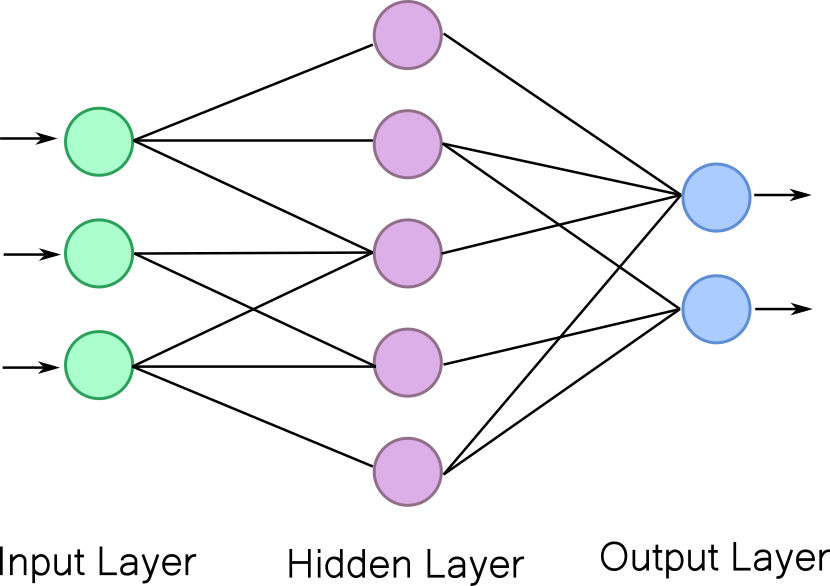
\includegraphics[width=0.6\linewidth]{ffnn}
    	\caption{Abstract structure of a feed-forward neural network. A real network will have many more layers and a lot more neurons per layer. Own figure.}
    	\label{fig:ffnn}
    \end{minipage}
	\hfill
	\begin{minipage}[t]{0.45\textwidth}
		\centering
		\begin{tikzpicture}[scale=0.5, transform shape]
  			\begin{axis}[scale only axis,
    					axis lines=middle,
    					inner axis line style={=>},
    					xlabel={},
    					ylabel={},
    					ytick={-1,-0.5,...,1},
    					xtick={-1,-0.5,...,1},
    					ymin=-1,
    					ymax=1,
    					xmin=-1,
    					xmax=1
  						] 
    			\addplot [mark=none,  blue,   ultra thick] {max(0, x)}; 
  			\end{axis}
		\end{tikzpicture}
    	\caption{Visualization of the ReLU activation function. Own figure.}
    	\label{fig:relu}
    \end{minipage}
\end{figure} 

\section{Neural Networks}

The following sections dissect the individual components of a neural network and explain concepts and procedures.

\subsection{Neuron}

A \textit{Neuron} is the smallest unit of a neural network and is essentially what the network is made up of. It computes the linear function 

\begin{align}
y = \sum\limits_{i=0}^kw_ix_i + b
\end{align}

where $w_i$ is the weight for the $i$-th input $x_i$ and $b$ is a bias. The weights and the bias are the values that can be learned during the training process of the network (see Section \ref{section:network_training}). The output of a layer of neurons of a network is the vector $(y_0, \cdots, y_t)$, $y_j$ being the output of the $j$-th neuron. Those outputs then serve as inputs to the next layer, although not every output has to be used by every next neuron. To prevent the network from collapsing into a single linear classifier and thus to increase the expressivity of the network, the output of a neuron is put into a non-linear so-called activation function. Although many different activation functions exist, most popular is the one called \textit{Rectified Linear Unit (\gls{relu})}, which was first presented by Jarrett et al. in \cite{relu}. The function is exemplarily visualized in \fig \ref{fig:relu} and is calculated as

\begin{align}
f(x) = max(0, x)
\end{align} 

\subsection{Feed-Forward Neural Network}

A \textit{Feed-Forward Neural Network} is a network consisting of layers of neurons. The first layer is called the input layer. Those are the neurons that receive the data that the network is supposed to process. The last layer is called the output layer. The output of the neural network depends on the design implied by the use case. It can be object coordinates like in our case, class probabilities in classification tasks or any other real-valued output. The intermediate layers are called hidden layers. Their number can grow to over a hundred in modern networks \cite{resnet}, thus the name deep neural networks and deep learning. All layers can have different numbers of neurons and connections to previous layers. A schematic overview over the structure of a neural network can be seen in \fig \ref{fig:ffnn}. A neural network can be seen as the function $y=f(x,\theta)$, where $\theta$ are the weights and biases of the neurons and some other parameters an $y$ is the output of the network.

\subsection{Convolutional Neural Networks}

\begin{figure}[!tbp]
	\centering
	\begin{subfigure}[t]{0.45\textwidth}
		\centering
    	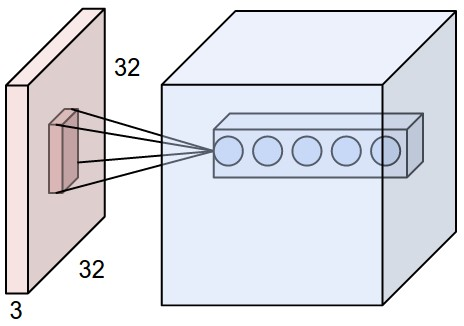
\includegraphics[width=0.7\linewidth]{conv_layer}
    	\caption{Example convolutional layer. The input image has dimensions 32x32 and 3 channels. The blue volume is the actual convolutional layer with multiple filters.}
    	\label{fig:conv_layer}
	\end{subfigure}
	\hfill
	\begin{subfigure}[t]{0.5\textwidth}
		\centering
    	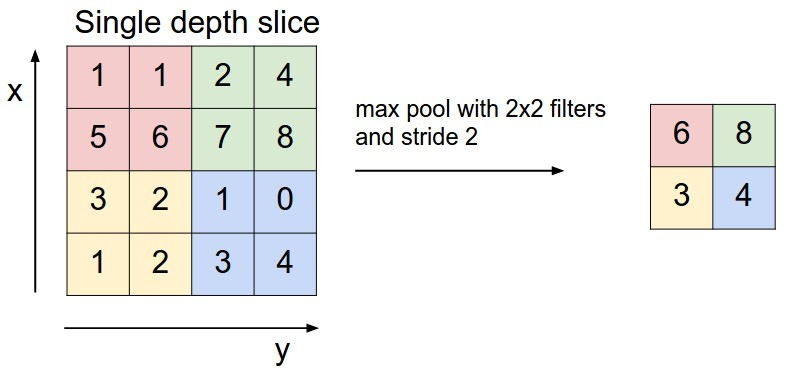
\includegraphics[width=0.9\linewidth]{pool_layer}
    	\caption{Example pooling layer with maximum as pooling operation.}
    	\label{fig:pool_layer}
	\end{subfigure}
	\caption{The two main layer types of a convolutional neural network.}
\end{figure} 

A \textit{Convolutional Neural Network (\gls{cnn})} describes a certain type of feed-forward neural network that consists of mainly two types of layers: \textit{Convolutional Layers} and \textit{Pooling Layers}. Normally, one or more convolutional layers are followed by a pooling layer. A convolutional layer convolves its input with a kernel which is moved along the input's dimensions. The kernel weights are shared, i.e. stay the same for the convolution of the whole input. \fig \ref{fig:conv_layer} shows the schematic of a convolutional layer. Each filter of the layer extends the output in the third dimension and has its own kernel. To reduce the size of the data a pooling layer can be added after the convolutional layer. This significantly speeds up computation and reduces the memory needed. It also reduces the number of parameters which helps to prevent the network from overfitting. An overfitted network performs well on the data it was trained on but does not generalize well, thus does not perform well on unseen data. Some architectures draw on a \textit{Fully-Connected Layer} as the last layer to perform the actual classification, etc. In such a layer every neuron is connected to every previous output. Convolutional neural networks are often used in computer vision tasks like image classification, instance segmentation and many more.

\subsection{Network training} \label{section:network_training}

When a network is created, usually its weights and biases are initialized to 0 or sampled randomly from a Gaussian distribution. To set the parameters to meaningful values that produce the desired output, the network has to be trained. We will now have a look at different techniques how to train a network.

\subsubsection{Error-Back Propagation} The predominant procedure to train a network is called \textit{Error-Back-Propagation} or \textit{Backpropagation}. To employ backpropagation, a differentiable but arbitrary loss function has to be defined. The loss function measures the error of the output of the network, e.g. by summing up the squared differences of the output and the objective output. The network is then applied to a training example in the so-called forward pass. Next, the loss function is derived with respect to each network weight using the chain rule of calculus. The derivative, the computed and the desired output together yield the change, also called delta, to be applied to the weights of the neuron. This delta is then propagated backwards through the net to calculate the deltas of the layers in between, again using the chain rule. After the deltas for all neurons have been computed, the weights are updated according to an update rule (see next paragraph). 

\subsubsection{Optimization} There exist many different patterns how to update the network weights after obtaining the detlas. The \textit{Stochastic Gradient Descent (\gls{sgd})} multiplies the delta by a learning rate and subtracts it from the weight. To ensure convergence, often the learning rate is decreased over time. A more elaborate method is the \textit{Adaptive Moment Optimization (Adam)} \cite{adam} which computes adaptive learning rates for each parameter. Here, an exponentially decaying average over past gradients as well as an exponentially decaying average over the past squared gradients serve to increase the learning rate in case of small gradients and decrease the learning rate in case of large gradients. Both averages are stored for the next iteration. Adam has greatly benefited the training process and proven to decrease computation time by finding local minima faster than \gls{sgd}. Other optimization procedures exist as well but will not be covered here.
	
\subsubsection{Regularization} Regularization can mean various things for neural networks. In general, its purpose is to keep the network from overfitting. Ian Goodfellow defined it in \cite{goodfellow} as any modification that reduces the generalization error but not the training error. Many network architectures regularize the net by adding a penalty term on the weights. Another possibility is to randomly deactivate a portion of the neurons to force the network to compensate the missing information, which is called \textit{Dropout}. \textit{Batchnormalization} helps the network generalize by subtracting the batch mean and batch standard deviation from the output of the previous layer. A batch is a subset of the input data which the network is trained with. This technique is often employed when the underlying machine can't fit the whole dataset in memory and because the network typically trains faster this way. To keep \gls{sgd} or other optimizers from reversing the covariance shift performed by batchnormalization the two parameters \textit{beta} and \textit{gamma} of such a layer are trainable.

\section{6D Pose Estimation}

\begin{figure}[!tbp]
	\centering
	\begin{subfigure}[t]{0.3\textwidth}
		\centering
    	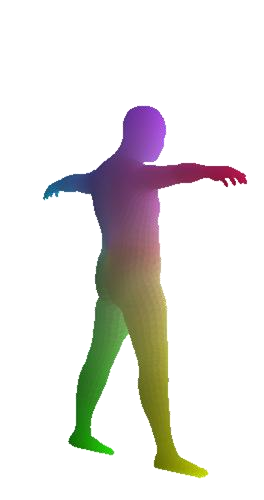
\includegraphics[width=0.45\linewidth]{human_object_coordinates}
    	\caption{The object coordinate representation of a human. Image from \cite{tsharp}.}
    	\label{fig:human_object_coordinates}
	\end{subfigure}
	\begin{subfigure}[t]{0.3\textwidth}
		\centering
    	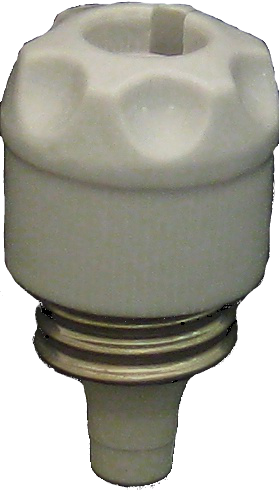
\includegraphics[width=0.45\linewidth]{tless_object}
    	\caption{An example object from the T-Less dataset. Image from \cite{tless}.}
    	\label{fig:tless_object}
	\end{subfigure}
	\begin{subfigure}[t]{0.3\textwidth}
		\centering
    	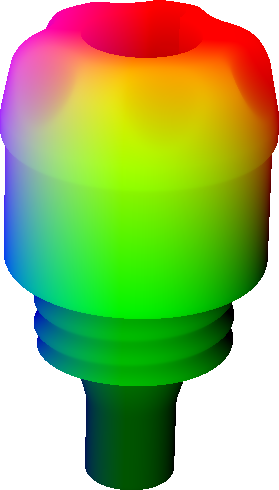
\includegraphics[width=0.45\linewidth]{tless_object_coordinates}
    	\caption{And the corresponding rendered 3D object coordinates (scaled for visualization). Own image.}
    	\label{fig:tless_object_coordinates}
	\end{subfigure}
	\caption{Example 3D coordinate representations.}
\end{figure} 

\textit{6D pose estimation} is a central task in the computer vision community. The goal is to retrieve an object's translation and rotation from an image, relative to the camera. \textit{6}D refers to the \textit{6-Degrees-of-Freedom (6-\gls{dof})}, i.e. the 6 free parameters of the \textit{3}D translation and \textit{3}D rotation. The field of application ranges from medical imaging, robotics, augmented reality, and many others. Different systems provide different accuracy. Setups using two cameras for stereo vision or depth information in addition to colors achieve good results. As endoscopes usually do not provide depth information or stereo vision, this work focuses on pose estimation using RGB-only images.

There are different possible ways to estimate the pose with learning-based approaches. The 6 parameters can be predicted directly or an intermediate representation can be used for pose computation. Predicting the parameters directly can be problematic, as the output of the neural network underlies noise and there is no possibility to verify or improve the pose afterwards. This is the reason why this work employs a network with a dense output, i.e. one output  for each pixel. The output for a pixel are the 3D coordinates on the object. Each subset of object coordinates leads to a certain pose. Some coordinates may contradict a pose and therefore the pose with the least contradictions is chosen as the best one. The next section will introduce this concept of so-called object coordinates in depth.

\subsection{Object Coordinate Regression} \label{objectcoordinates}

\begin{figure}[!tbp]
	\centering
    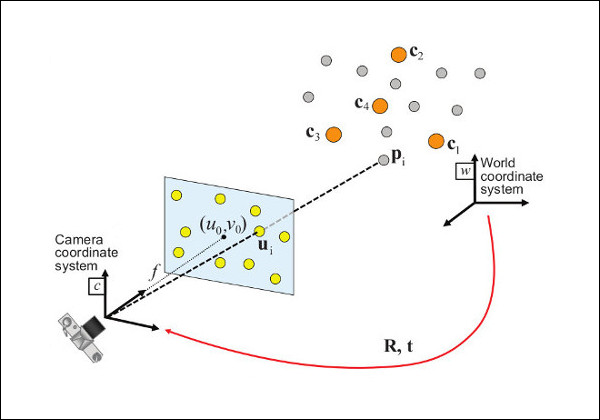
\includegraphics[width=0.45\linewidth]{pnp}
    \caption{The relationship between the camera, the 3D points and their projections on the screen using the rotation matrix $R$ and the translation vector $t$. Image from \cite{opencv_pnp}.}
    	\label{fig:pnp}
\end{figure} 

Tayler et al. first used object coordinates in \cite{tsharp}. Instead of directly predicting the location of joints or limbs of the human body they computed for each pixel the corresponding 3D location on the person (see \fig \ref{fig:human_object_coordinates}). The idea can be transfered to objects of any kind. \fig \ref{fig:tless_object} shows an example object from the T-Less dataset \cite{tless} and \fig \ref{fig:tless_object_coordinates} shows the corresponding rendered 3D object coordinates.


TODO: this is not entirely correct
The 3D coordinates and the respective 2D pixel locations on the image yield the \textit{Perspective-n-Point (\gls{pnp}) Problem}. That is, for a given pixel $p$ on the image and the corresponding 3D point $x$ (both in homogeneous coordinates), a pose consisting of the rotation matrix $R$ and the translation vector $t$ has to fulfill the following equation

\begin{align}
 p = K \ [ \ R \ | \ t \ ] \ x \label{eq:pose_projection}
\end{align} 

where $K$ is the camera matrix

\begin{align}
K = \begin{bmatrix}
f_x & s & c_x \\
0 & f_y & c_y \\
0 & 0 & 1 
\end{bmatrix}
\end{align}

which projects the 3D point transformed into the camera coordinate system on the 2D image plane. $s$ is a skew factor which is usually $0$, $(c_x, c_y)$ is the principal point, usually the center of the image and $f_x$ and $f_y$ is the focal lengths in $x$ and $y$ direction respectively. The values for those variables can vary when for example cropping the image. \fig \ref{fig:pnp} visualizes the relation of pixels and object coordinates. If equation \ref{eq:pose_projection} is overdetermined because there are more correspondences than variables it cannot be solved directly.

A method to solve the \gls{pnp} problem for many correspondences is to use the \textit{\gls{ransac} algorithm} \cite{ransac}. \gls{ransac} selects a model based on a subset of the dataset and evaluates it against the remaining data. This way the approximate best model is found iteratively. Algorithm \ref{algorithm:ransac} shows the outline of the \gls{ransac} algorithm for pose estimation. The energy function can be varied. It can for example be the number of inliers. Inliers are 3D points whose reprojected 2D location is within a certain area of the actual 2D location. Since \gls{ransac} is well known and employed in many different applications to estimate a model that fits a dataset best, we use it in this work to compute the pose. The implementation that is used is the one incorporated into the \textit{solvePnPRansac} method of the \textit{OpenCV} \cite{opencv} framework. 

\begin{algorithm}
\caption{RANSAC} \label{algorithm:ransac}
\begin{algorithmic} 
\REQUIRE Set of 3D points
\REQUIRE Set of corresponding 2D points
\REQUIRE Number of iterations $i$
\REQUIRE An energy function to score the pose hypothesis $E$
\STATE Set current energy $e=0$
\STATE Set current best pose hypothesis $h$ to $null$
\FOR{$1 ... i$}
\STATE Select a subset of corresponding points to compute pose $H$
\STATE Compute energy of the pose $e'=E(H)$
\IF{$e' > e$}
\STATE Store pose $H$ as current best in $h$
\STATE Set $e = e'$
\ENDIF
\ENDFOR
\RETURN Best pose $h$
\end{algorithmic}
\end{algorithm}
\chapter{Related Work}

In the following section, we investigate the current state of research on 6D pose estimation. The chapter starts with an excerpt of non-learning-based methods. We then present more recent, learning-based works with emphasis on active learning and fine-tuning of neural networks.

\section{Research on 6D Pose Estimation}

Pose estimation has become an increasingly interesting problem with the advent of robots in production and the area of virtual and augmented reality \cite{bb8}. Research before the rise of learning-based methods focused on manual feature extraction, divided into the major groups of sparse, dense and template-based approaches. Nowadays scientists often employ learning-based techniques which offer higher accuracy.

\subsection{Non-Learning-Based}

Before the major breakthrough of deep learning in 2012 \cite{alexnet}, handcrafted feature-based approaches were common for 6D pose estimation \cite{ylecun}. A lot of research matches sparse characteristics detected in the image against a database that contains the related pose information. The works of \cite{dglowe1, dwagner} use keypoints as the discriminative feature and offer good accuracy on well-textured objects. Unfortunately they yield bad performance on poor-textured or texture-less objects, because in those cases detectors are unable to find stable keypoints or any at all. The methods presented in \cite{gklein,dglowe2,charris} identify edges in the image and use different techniques to obtain an initial pose guess based on them. The resulting pose is retrieved by iteratively refining the previous guess, by minimizing the distance of the projected and detected edges.
\nnewline
Template-based methods \cite{hinterstoisser1, hinterstoisser2, rioscabrera, csteger} use generated views of discrete viewopints on the object at different angles which are matched against the given image to retrieve the pose. This approach relies mainly on the shape of objects and thus works well for poor-textured or textureless objects. To cover many objects and a large pose range the number of templates of an object has to be increased though, which slows down prediction. Hashing the views to speed up the pose estimator reduces accuracy \cite{zhou}. Additionally, deformed or occluded objects decrease precision, as templates globally reason about the object's pose.
\nnewline
Some authors draw on additional views to improve accuracy. Stereo camers are used in \cite{kpauwels}. A second image from another angle implies depth information to a certain extend but involes the additional task of stereo matching. The sudden availability of cheap depth sensors, like the Kinect, gave rise to algorithms making use of RGB-D images. Multiple approaches are possible when incorporating depth to retrieve an object's pose. Voting schemes were employed in \cite{bdrost, salasmoreno} and achieved good. First, a reference point in the image is selected and paired with all other points. The point pair feature called pair then votes for a possible pose, if their distance and respective normals are contained in the global sparse model description. The pose with the most votes is deemed to be the optimal one.

\subsection{Learning-Based}

Methods that learn information about objects - that is not explicitly modeled - started to outperform the previous techniques. There exist a vast literature for this task but we restrict our review to recent works that are most relevant to our approach.
\nnewline
Lai et al. use decision tress in \cite{klai}, which incorporate the semantic information of objects and their poses. Tom{\`{e}} et al. predict human poses from single RGB images in an end-to-end fashion \cite{dtome}. The system of \cite{azeng} relies on multi-view images and depth information and scored the 3rd and 4th place in the Amazon Picking Challenge 2016 \cite{apc}. A prominent example of the problem of camera localization, which is estimating the camera position in 3D space relative to the scene, is PoseNet \cite{posenet}. The underlying architecture of the employed neural network is based on GoogleNet, which was introduced in \cite{googlenet}. The CNN estimates the camera position from a single image in an end-to-end fashion and is fast, but, with an error of 50 centimeters in some cases, too inaccurate to reliably estimate poses of surgical tools.

\paragraph{BB8.}

The recently developed BB8 \cite{bb8}, which is an abbreviation for the 8 corners of the bounding-boxes of objects, is the result of the work of Rad and Lepetit that operates on RGB-only images. Instead of regressing the pose of an object with object coordinates like \cite{brachmann1}, they let a deep neural network estimate the object segmentations first and then predict the 2D locations of the 3D corners of the object's bounding box. 
\nnewline
\begin{figure}[!tbp]
	\centering
	\begin{subfigure}[b]{0.45\textwidth}
		\centering
    	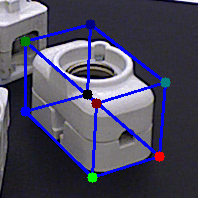
\includegraphics[width=0.45\linewidth]{bb8}
    	\caption{The control points of the object's bounding box.}
	\end{subfigure}
	\hfill
	\begin{subfigure}[b]{0.45\textwidth}
		\centering
    	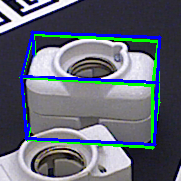
\includegraphics[width=0.45\linewidth]{bb8_prediction}
    	\caption{The final estimated pose. Green is the groundtruth.}
	\end{subfigure}
	\caption{Example images displaying the functioning of BB8. Images taken from \cite{bb8}.}
\end{figure}
Despite its differences to \cite{brachmann1}, the object's position is not predicted directly either, but instead regressed by solving the perspective-n-point (PnP) problem of the correspondences of the corners of the object's bounding box and the projected 2D locations of the corners predicted by the network. The architecture of the first and second net is based on VGG \cite{vgg} respectively but with the last layer cut off and replaced by a fully connected layer which is fine-tuned. 
\nnewline
The first network, which segments the image, helps estimating the pose of the object in a way that the second network positions its window at the center of the segmentation and predicts the pose. The pose prediction works by estimating the 2D locations of the 3D corners of the object's bounding box. The network reasons globally about the object by not moving the window containing the object during training and prediction. The authors argue that patch-based pose estimators are typically very noisy, and hence require a robust optimization scheme, like RANSAC. 
\nnewline
Unfortunately, BB8's take on pose estimation fails on symmetric objects, when implemented directly as described above. To address this problem, the authors first estimate the rotational angle of the object, and mirror the image if necessary. This way, a CNN can be trained only on a certain range of the angle of the pose.
\nnewline
The proposed method offers good performance and can compete with and partly surpasses state-of-the-art research. Yet, object coordinates provide high accuracy too and due to the assumption of the author of this work, that the often merely patch-wise visibility of the surgical instruments calls for a non-global reasoning design BB8 is followed any further in this work.

\paragraph{SSD-6D.}

The system presented in \cite{ssd-6d} is based on the work in \cite{ssd}, called Single-Shot Multibox Detector, or short SSD. Their take on 6D pose estimation is especially alluring, as the authors train the network exclusively on synthetic data. A positive outcome would imply that the lack of already annotated datasets for 6D pose estimation could be overcome by generating data for network training. 
\nnewline
Kehl et al. let the network estimate the probability of a discrete viewpoint on the object. Those viewpoints are sampled equidistant alongside a predefined degree step-size to represent all possible poses of the objects. This view estimate, combined with an estimate on the rotation, is used to generate pose predictions. 
\nnewline
\begin{figure}[!tbp]
	\centering
	\begin{subfigure}[b]{0.3\textwidth}
		\centering
    	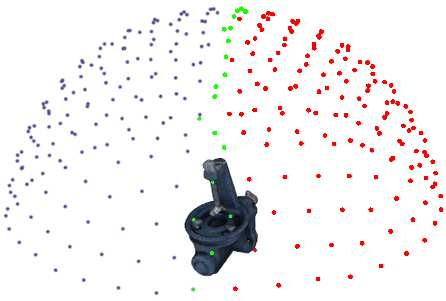
\includegraphics[width=\linewidth]{ssd_6d_sphere}
    	\caption{An exampe of a discrete distribution of viewpoints on an object.}
	\end{subfigure}
	\hfill
	\begin{subfigure}[b]{0.6\textwidth}
		\centering
    	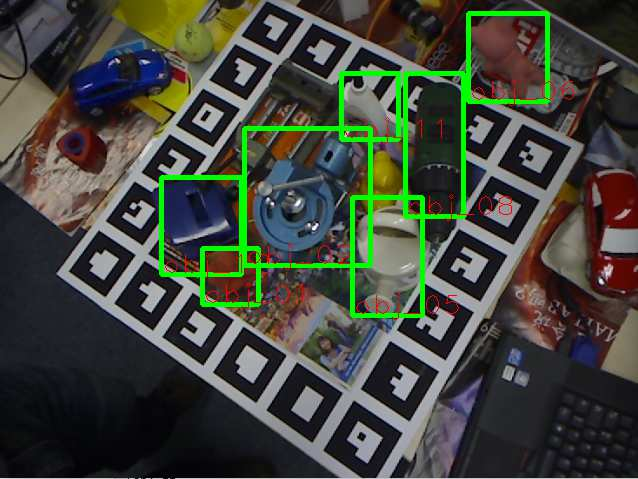
\includegraphics[width=0.45\linewidth]{ssd_6d_bb}
    	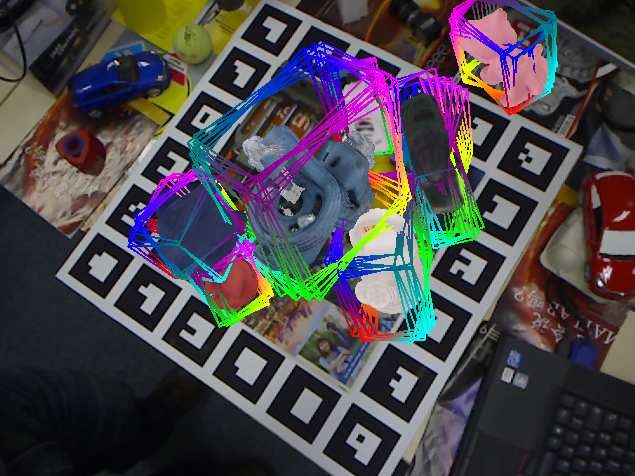
\includegraphics[width=0.45\linewidth]{ssd_6d_pose}
    	\caption{Left image: An example for bounding boxes found by the SSD-6D network. Right image: The most confident views and rotations for those boxes.}
	\end{subfigure}
	\caption{Example images displaying the functioning of SSD-6D. Images taken from \cite{ssd-6d}}
\end{figure}
The SSD-inspired network architecture produces feature maps that are convolved to predict the class, 2D bounding box, viewpoint scores and in-plane rotation of an object. The network is trained entirely on images from the MS COCO dataset \cite{mscoco} with the objects to be detected rendered into with arbitrary translations and rotations. For each transformation, the network is given the closest discrete viewpoint, in-plane rotation and the tightest bounding box as a regression target.
\nnewline
The author's reasoning, that their approach on pose estimation is a more natural one than pose regression stands to reason, as a human learns what an object looks like by viewing it from different angles. Nevertheless, the network produces rather inaccurate initial results.  To remedy this drawback, an optimization scheme extracts 3D contour points from the rendered hypothesis and minimizes the distance to the detected 2 locations of the points on the image. 
\nnewline
Since the neural network alone performs less well compared to \cite{brachmann1} or \cite{bb8} and the approach requires an optimization process, which could also be applied to the two mentioned works, it is not investigated further. 

\paragraph{Kurmann et al.}

The work of \cite{kurmann} estimates poses of surgical instruments in minimally invasive surgery. Similarly to object coordinate regression, Kurmann et al. develop a system that produces probabilities of the presence of an object but not in a dense way but instead only for the joints of the tools. Their design draws on a scene model which holds how many tools can be visible at most, what tools are currently visible and what parts of those tools.
\nnewline 
The authors of that paper argue that the common two-stage pipeline for 6D pose estimation, that consists of object detection and then pose estimation, results in a more complicated design, and criticize that a sliding window approach might miss very small or very large instruments, i.e. advocate a global reasoning design.
\nnewline
The architecture of the employed network is based on the U-Net developed by the authors of \cite{oronneberger}, and trained by optimizing the cross-entropy derived from the scene model described earlier. The network architecture of U-Net is extended by a fully connected layer that is trained to predict the probabilities of the instruments.
\nnewline
The results of the design look promising and run time per image is around $100 ms$, enabling it to be deployed as a real-time solution. Conversely, mainly literature of the biomedical imaging was considered and compared, disregarding research work in other areas on pose estimation.

\subsection{Learning-Based: Object Coordinate Regression}

An interesting section of learning-based pose estimation are the works employing the method of so-called object coordinate regression (see Section \ref{objectcoordinates}). The idea is based on \cite{tsharp} and \cite{firstcoordinateregression}. The first used it to estimate the pose of a human body, the latter to regress the cameras position in a scene retrieved from a single RGB-D image.
\nnewline
Brachmann et al. achieved record-breaking results in \cite{brachmann1} for texture-less objects and good performance in general. The authors based their work on forests instead of trees to regress the object's pose. The forests are trained to jointly predict the probability of object instances as well as the object coordinate probability for a given pixel. The output of the forest is processed in an energy function that imposes an energy minimization problem to regress the object's pose. A RANSAC-like scheme then iteratively refines the pose.
\nnewline
In \cite{brachmann2}, Brachmann et al. adjusted their pipeline from \cite{brachmann1} to work with RGB-only images. To reduce uncertainty in the object instance and coordinate predictions they incorporate an auto-context framework and marginalize the object coordinates over the depth information to cope with the missing fourth channel. The presented system outperforms Brachmann et al.'s previous work but is still based on forests. 
\nnewline
Krull et al. elaborated \cite{brachmann1} by replacing the energy function by a CNN \cite{akrull}. They were able to further improve the performance and transfer object coordinate regression to modern deep neural networks. The system called PoseAgent fuses regression forests and CNNs \cite{poseagent}. The regression forest outputs pose hypotheses that the CNN then refines. Krull et al. are able to achieve state-of-the-art results and improve resource utilization. Although \cite{trees-vs-cnn} finds, that random forests partly offer a slightly superior performance, neural networks can compete and are therefore the focus of this work.

\paragraph{Pertsch.}

Although \cite{pertsch} also works with RGB-D images, we present his work here as the author proposes an easy extension to adapt the entire process to RGB-only images and presents promising results. The work by Pertsch is based on \cite{brachmann1}, i.e. uses object coordinates  (see section \ref{objectcoordinates}), but replaces the random forest with a CNN. The developed pose estimation pipeline relies on three steps. The first one segments the image, the second regresses the object coordinates, and the last one evaluates pose hypotheses. 
\nnewline
We don't to go into detail into the first operation of the pipeline as our training and test data already includes segmentations and we can hence omit it completely. The second stage consists of a multilayer CNN-architecture to predict the object coordinates. The architecture consists of an encoder-decoder multilayer network. Inspired by \cite{oronneberger}, the author assimilates skip-layer connections. The network computes object coordinates for each pixel of the previously computed segmentation. Pertsch employs a RANSAC-scheme to improve the quality of the predicted final pose. Two different methods to retrieve the pose are presented in the work, one relying on the energy function introduced in \cite{brachmann1} but in an altered version, and one procedure solely drawing on RGB information without the additional depth of a sensor. The latter, which is more relevant for us as we do not have any depth readings, is based on the earlier presented \cite{brachmann2}. 
\nnewline
Instead of penalizing depth divergences of the rendered depth from the estimated pose and the sensor readings, the number of pixels whose reprojection error is greater than a certain threshold is minimized iteratively by the RANSAC algorithm. This allows for the RGB-only extension that the author suggests but does not elaborate in detail. Without depth the pose regression becomse a PnP problem, that can be solved by a PnP solver which takes at  four 3D-2D point correspondences as input. We pursue a similar approach in our work which differs in architecture of the network, the steps of the pipeline and the input data. But the general ideas of \cite{pertsch} and especially \cite{brachmann1} are adopted and further complemented with current research and active and incremental learning.

\section{Research on Active and Online Learning}

Online learning considers how to incorporate new available data into a trained model or neural network. Active learning is the field of selecting data that a human should annotate manually, because the model does not perform well on it. The literature survey \cite{activesurvey} gives an overview over methods developed before 2011. Wang and Shang, the authors of \cite{dwang}, might be among the first to incorporate active learning into deep learning though, according to \cite{zhou}. In \cite{hyperspectral}, Al Rahhal et al. apply a similar idea to hyperspectral image classification, a task that shares the foibles to be tedious and time-consuming with biomedical image annotation. The authors developed an active selection paradigm to electrocardiogram classification. 

\paragraph{Zhou et al.}

In \cite{zhou}, Zhou et al. describe a novel process of actively demanding data to be annotated to improve the network quality and apply the newly available data in an incremental manner. They focus on this area because annotating biomedical images is still a time-consuming task that requires a lot of expertise and skill.
\nnewline
Opposed to retraining from scratch, the network is fine-tuned by an incremental tuning algorithm. According to the authors, researchers have shown that this offers superior performance. In contrast to our task, the authors want to achieve improvements on image classification and frame detection, but work on biomedical images nonetheless.
\nnewline
\begin{figure}[!tbp]
	\centering
    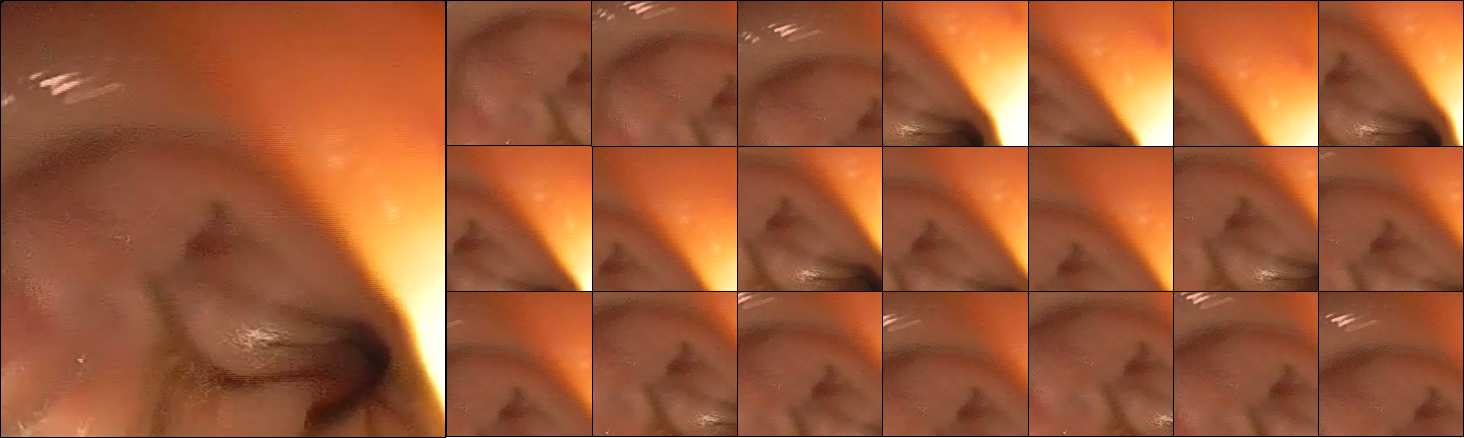
\includegraphics[width=0.7\linewidth]{fine_tuning}
	\caption{A candidate (left) and the patches generated sharing the same label. \cite{zhou}}
	\label{fig:zhou}
\end{figure}
Computer-aided-diagnosis (CAD) systems usually provide a candidate generator, which can quickly produce candidates, including true and false positives, to train with. Through data augmentation the learner can be made more robust to unforeseen situations. For this, numerous patches sharing the same label are generated from the candidate, as can be seen in Figure \ref{fig:zhou}, an presented to the classifier. 
\nnewline
The active selection process of candidates requires a measure of the worthiness of a candidate. To achieve this, the entropy and diversity of patches are calculated using the network's predictions for the patches of a candidate. Entropy is the negative log-likelihood of the network's prediction, whereas diversity captures how much patches of a candidate contradict, as they should all share the same label. Candidates with contradicting patches or low entropy can be selected for manual annotation.
\nnewline
The procedure quickly improves the neural network's accuracy. Learning from scratch or random selection of next candidates are quickly  outperformed, as only around 20\% of manually annotated candidates are necessary to reach the same error rate with the presented procedure.
\nnewline
In our case, data augmentation is possible, as we can render synthetic images, but the unnatural lightning and shadowing might decrease the accuracy of the design. The question of how to find  a worthiness measure arises too, as we can't directly tell how sure a network is when predicting a pose. But it provides a good direction of how to approach active learning.

\paragraph{Liu \& Ferrari.}

\begin{figure}[!tbp]
	\centering
    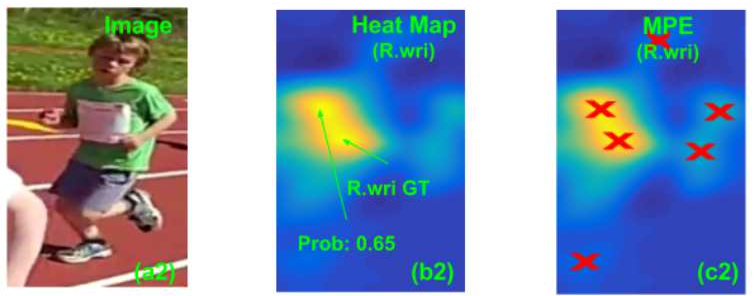
\includegraphics[width=0.6\linewidth]{human_pose_heatmap}
    \caption{An image of a human body, the corresponding heatmap as well as the result of the Multiple Peak Entropy (MPE). \cite{humanpose}}
    \label{fig:humanpose}
\end{figure}
In \cite{humanpose}, Liu and Ferrari describe new strategy for active learning for human pose estimation, a time-consuming task to produce groundtruth annotations for. Their key contributions consist of an uncertainty estimator for the joint predictions produced by a convolutional pose machine, and an annotation interface that reduces the time needed by a human annotator to click joints.
\nnewline
The active learning scheme incorporates influence and uncertainty cues. Influence cues consider images that are similar to other unlabeled images could propagate information. The uncertainty cues are measured by the uncertainty estimator. The estimator focuses on uncertain predictions, i.e. predictions with multiple weak peaks (multiple peak entropy). The functioning of the estimator can be seen in Figure \ref{fig:humanpose}. The final selection process then takes both cues into account when requesting an image to be manually annotated.
\nnewline
In addition, an interface is proposed that reduces the annotation time significantly. The system predicts a pose and segments the image around joints. The user can then right click anywhere in the segmentation to accept the estimated joint location or manually select it.
\nnewline
The results of \cite{humanpose} look auspicious, as a reduction in annotation time can be achieved through the interface and the selection process. Regrettably, it cannot be directly applied to our problem, as we need a problem-specific certainty estimator. But the idea of requesting similar images to be annotated might yield a performance gain, and similarly to the presented interface we present the user with an initial probable pose, too, to make only small corrections necessary.
\chapter{Manual Annotation} \label{chapter:manual_annotation}

\begin{figure}[!tbp]
	\centering
    
\includegraphics[width=\linewidth]{6dpat}
    \caption{The logo of the pose annotation tool 6D-PAT. Own image.}
    	\label{fig:6dpat_logo}
\end{figure} 

The following chapter analyzes manual 6D pose annotation process and its prerequisites. To this end, the necessary terminology is defined and explained and the workflow to annotate poses using the developed annotation tool is described. The assessment of the requirements of the annotation procedure and the creation of the tool are conducted based on the medical image dataset, which is described further below.

\section{Terminology} \label{section:terminology}

\textbf{Image.} An image $I$ is a 2D matrix of pixels. The pixel $u$ at position $(i, j)$ is referenced by the tuple $(x, y)$, where $x = j$ and $y = i$. The inverted notation is chosen over the common row-major matrix indexing to account for the universal  \\

\noindent\textbf{Object Model.} An \textit{object model}, or \textit{3D model}, $O$ is composed of a set of points $M \subseteq \mathbb{R}^3$ and a set of triangles $T = \{(m_1, m_2, m_3) \in M^3\}$, also called mesh. The real-world entity that the object model resembles is not restricted. In case of the T-Less dataset \cite{tless} the objects are mainly hardware like screws and power sockets. \\

\noindent\textbf{6D Pose.} A \textit{6D pose} $P$ is the tuple $(R, t)$, where $R$ is the 3x3 rotation matrix and $t$ the translation vector used to transform the respective object model into camera coordinates (see section \ref{objectcoordinates} for details). \\

\noindent\textbf{Correspondence.} A \textit{correspondence} $C$ is the tuple $(u, p)$, which captures the relation between a pixel $u$ of an image $I$ and an object model $O$. The pixel $u$ is the projection of the 3D point $p$ onto the image plane using the camera matrix $K$ and a pose $P$. If the pose is unknown, a set of at least three correspondences can be used to retrieve the pose computationally (see section \ref{objectcoordinates} for details). \\

\noindent\textbf{Segmentation Mask.} A \textit{segmentation mask} (or \textit{segmentation image}) $S$ for an image $I$ is a second image of the same size. Each position $(x, y)$ of the mask encodes the class of the pixel at $(x, y)$ in $I$. The set of classes can be defined arbitrarily. In the context of this work each class represents a type of object model. The segmentation mask can be seen as the mapping $s(x, y) = q_i$ for a class set $Q = \{q_0, \cdots, q_n\}$. \\

\noindent\textbf{Pose Recovery.} The process of recovering a pose $P$ of an object model $O$ visible in the image $I$ can be performed in various ways. In this work the key operation is to create a set of 2D-3D correspondences and solve the respective perspective-n-point problem. \\

\noindent\textbf{Ground-Truth.} A \textit{ground-truth pose} $\bar{P}$ is a 6D pose. A ground-truth pose is always created by a human instead of a machine. The ground-truth pose is the best approximation of the rotation and translation of an object model $O$ on an image $I$ of said object. It is an approximation because there can be a discrepancy between the real world object and its digital 3D representation. Distortions by the camera used to photograph the object and other influences might also not be modeled correctly or not accounted for at all. The rotation and translation error of a ground truth pose are bearable and thus are the objective for neural networks.

\begin{figure}[!tbp]
	\centering
	\begin{subfigure}[t]{0.47\textwidth}
	\centering
    	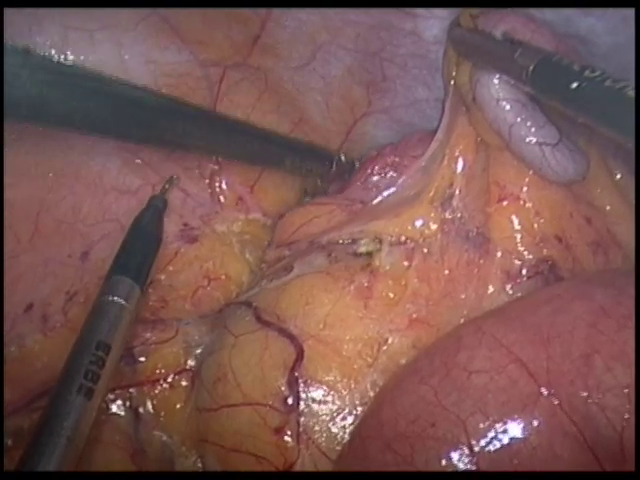
\includegraphics[width=0.8\linewidth]{sfb_original}
    	\caption{An example image from the medical dataset. Image from TODO: cite.}
    	\label{fig:sfb_original}
	\end{subfigure}
	\hfill
	\begin{subfigure}[t]{0.47\textwidth}
	\centering
    	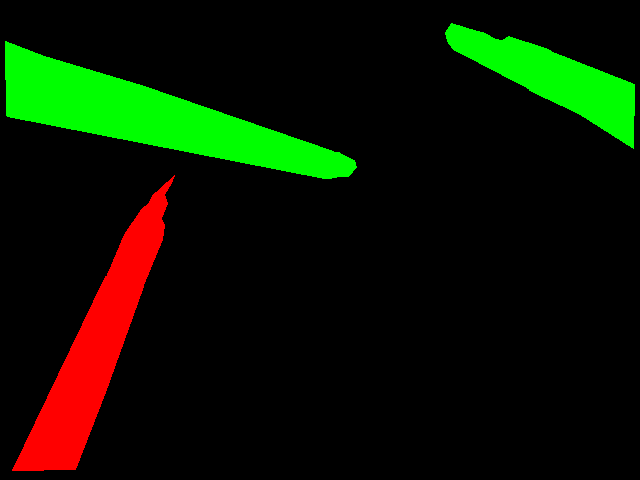
\includegraphics[width=0.8\linewidth]{sfb_segmentation}
    	\caption{The corresponding segmentation mask to the image in fig \ref{fig:sfb_original}. The colors encode the tools' classes. Taken from TODO: cite.}
    	\label{fig:sfb_segmentation}
	\end{subfigure}
	\caption{An example image and its corresponding segmentation mask from the medical dataset.}
	\label{fig:sfb}
\end{figure} 

\section{Medical Images}

The goal of this work is to provide a system to successfully and efficiently annotate the medical images that were provided upfront. The dataset includes segmentation masks but no object models or existing pose annotations. An example image together with the corresponding segmentation mask are given in \fig \ref{fig:sfb}. The dataset resembles the characteristics and quality of images from laparoscopic videos, i.e. there is no depth information present and occlusion and artifacts like motion blur can occur. The issues with this dataset are discussed in section \ref{section:6dpat_difficulties}. 

\section{6D Pose Annotation Tool (6D-PAT)}

\begin{figure}[!tbp]
	\centering
	\begin{subfigure}[t]{0.47\textwidth}
		\centering
    	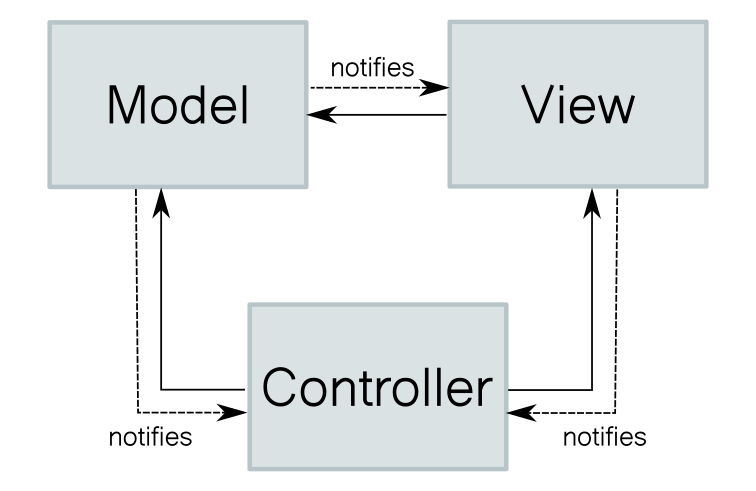
\includegraphics[width=0.8\linewidth]{mvc}
    	\caption{The Model-View-Controller architecture. The solid lines stand for a direct connection either because the target is owned or known by reference. The dashed line is an indirect connection using for example the observer pattern or the Qt Signals and Slots mechanism visible in \fig \ref{fig:qt_signals_slots}. Own image.}
    	\label{fig:mvc}
	\end{subfigure}
	\hfill
	\begin{subfigure}[t]{0.47\textwidth}
	\centering
    	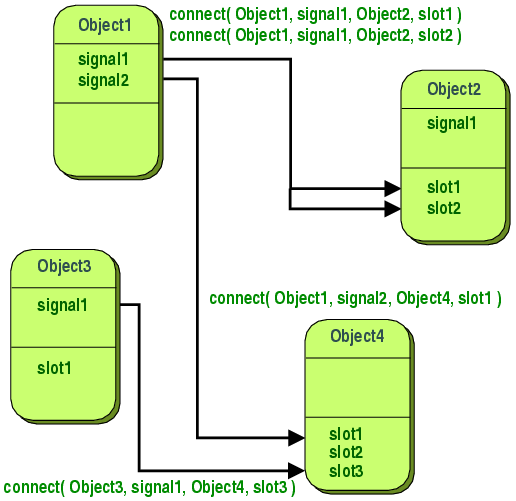
\includegraphics[width=0.8\linewidth]{qt_signals_slots}
    	\caption{The Signals and Slots mechanism of Qt. A class can define signals it can emit, independently of any listeners waiting for that signal. Slots are the functions that, when connected a signal, are called and can thus react to the signal. Image from \cite{qt_signals_and_slots}.}
    	\label{fig:qt_signals_slots}
	\end{subfigure}
	\caption{Two basic architectural concepts used in \gls{6dpat}: the model view controller pattern and the signal and slots pattern.}
\end{figure} 

The creation of sufficient training data for neural networks can be a time-consuming and tedious process. Using non-specialized tools designed for other purposes, like 3D modeling programs, require the personnel creating the annotations to get accustomed to complex user interfaces (\gls{ui}s). The goal of the annotation tool is to provide a system that allows easy and efficient annotation of images, images of the medical dataset in particular. The annotated poses, the so-called \textit{Ground-Truth Poses} (see section \ref{section:terminology}), can later be used to train a neural network. The program is written in the language C++ and named \textit{6D - Pose Annotation Tool (\gls{6dpat})}. Its logo can be seen in \fig \ref{fig:6dpat_logo}. Although the program was developed using the \textit{Linux}-based operating system \textit{Ubuntu}, it is compilable on other systems as well.

\subsection{Frameworks \& Third-Party Libraries}

The listed frameworks are all necessary dependencies of the annotation tool. There are no dependencies other than the mentioned ones. They are not part of the repository but have to be compiled individually instead. Since all three frameworks/libraries are platform-independent the program can be compiled and run on different systems. \\

\noindent\textbf{Qt.} \textit{Qt} \cite{qt} is a powerful framework for C++ that offers a vast selection of user interface components but also general functionality that exceeds the capabilities of the standard C++ library. Qt is also chosen as the main framework because it ensures portability of C++ applications by encapsulating system calls of all kind. The program \textit{Qt Creator} is the \textit{Integrated Development Environment (IDE)} that is included in the Qt distribution was used to write and execute the code of \gls{6dpat}. An IDE combines an editor to edit code an some environment to execute it. \\

\noindent\textbf{OpenGL.} \textit{OpenGL} \cite{opengl} is a widespread open-source 3D graphics library specification. Implementations for many operating systems exist, thus making most OpenGL using applications compilable in different environments without further modifications. \textit{Mesa 3D} \\

\noindent\textbf{OpenCV.} \textit{OpenCV} \cite{opencv} is a C++ library created for various computer vision tasks, hence the name. OpenCV provides implementations for tracking, object detection, segmentation and many more. In this work its \textit{solvePnPRansac} is used. \\

\begin{figure}[!tbp]
	\centering
    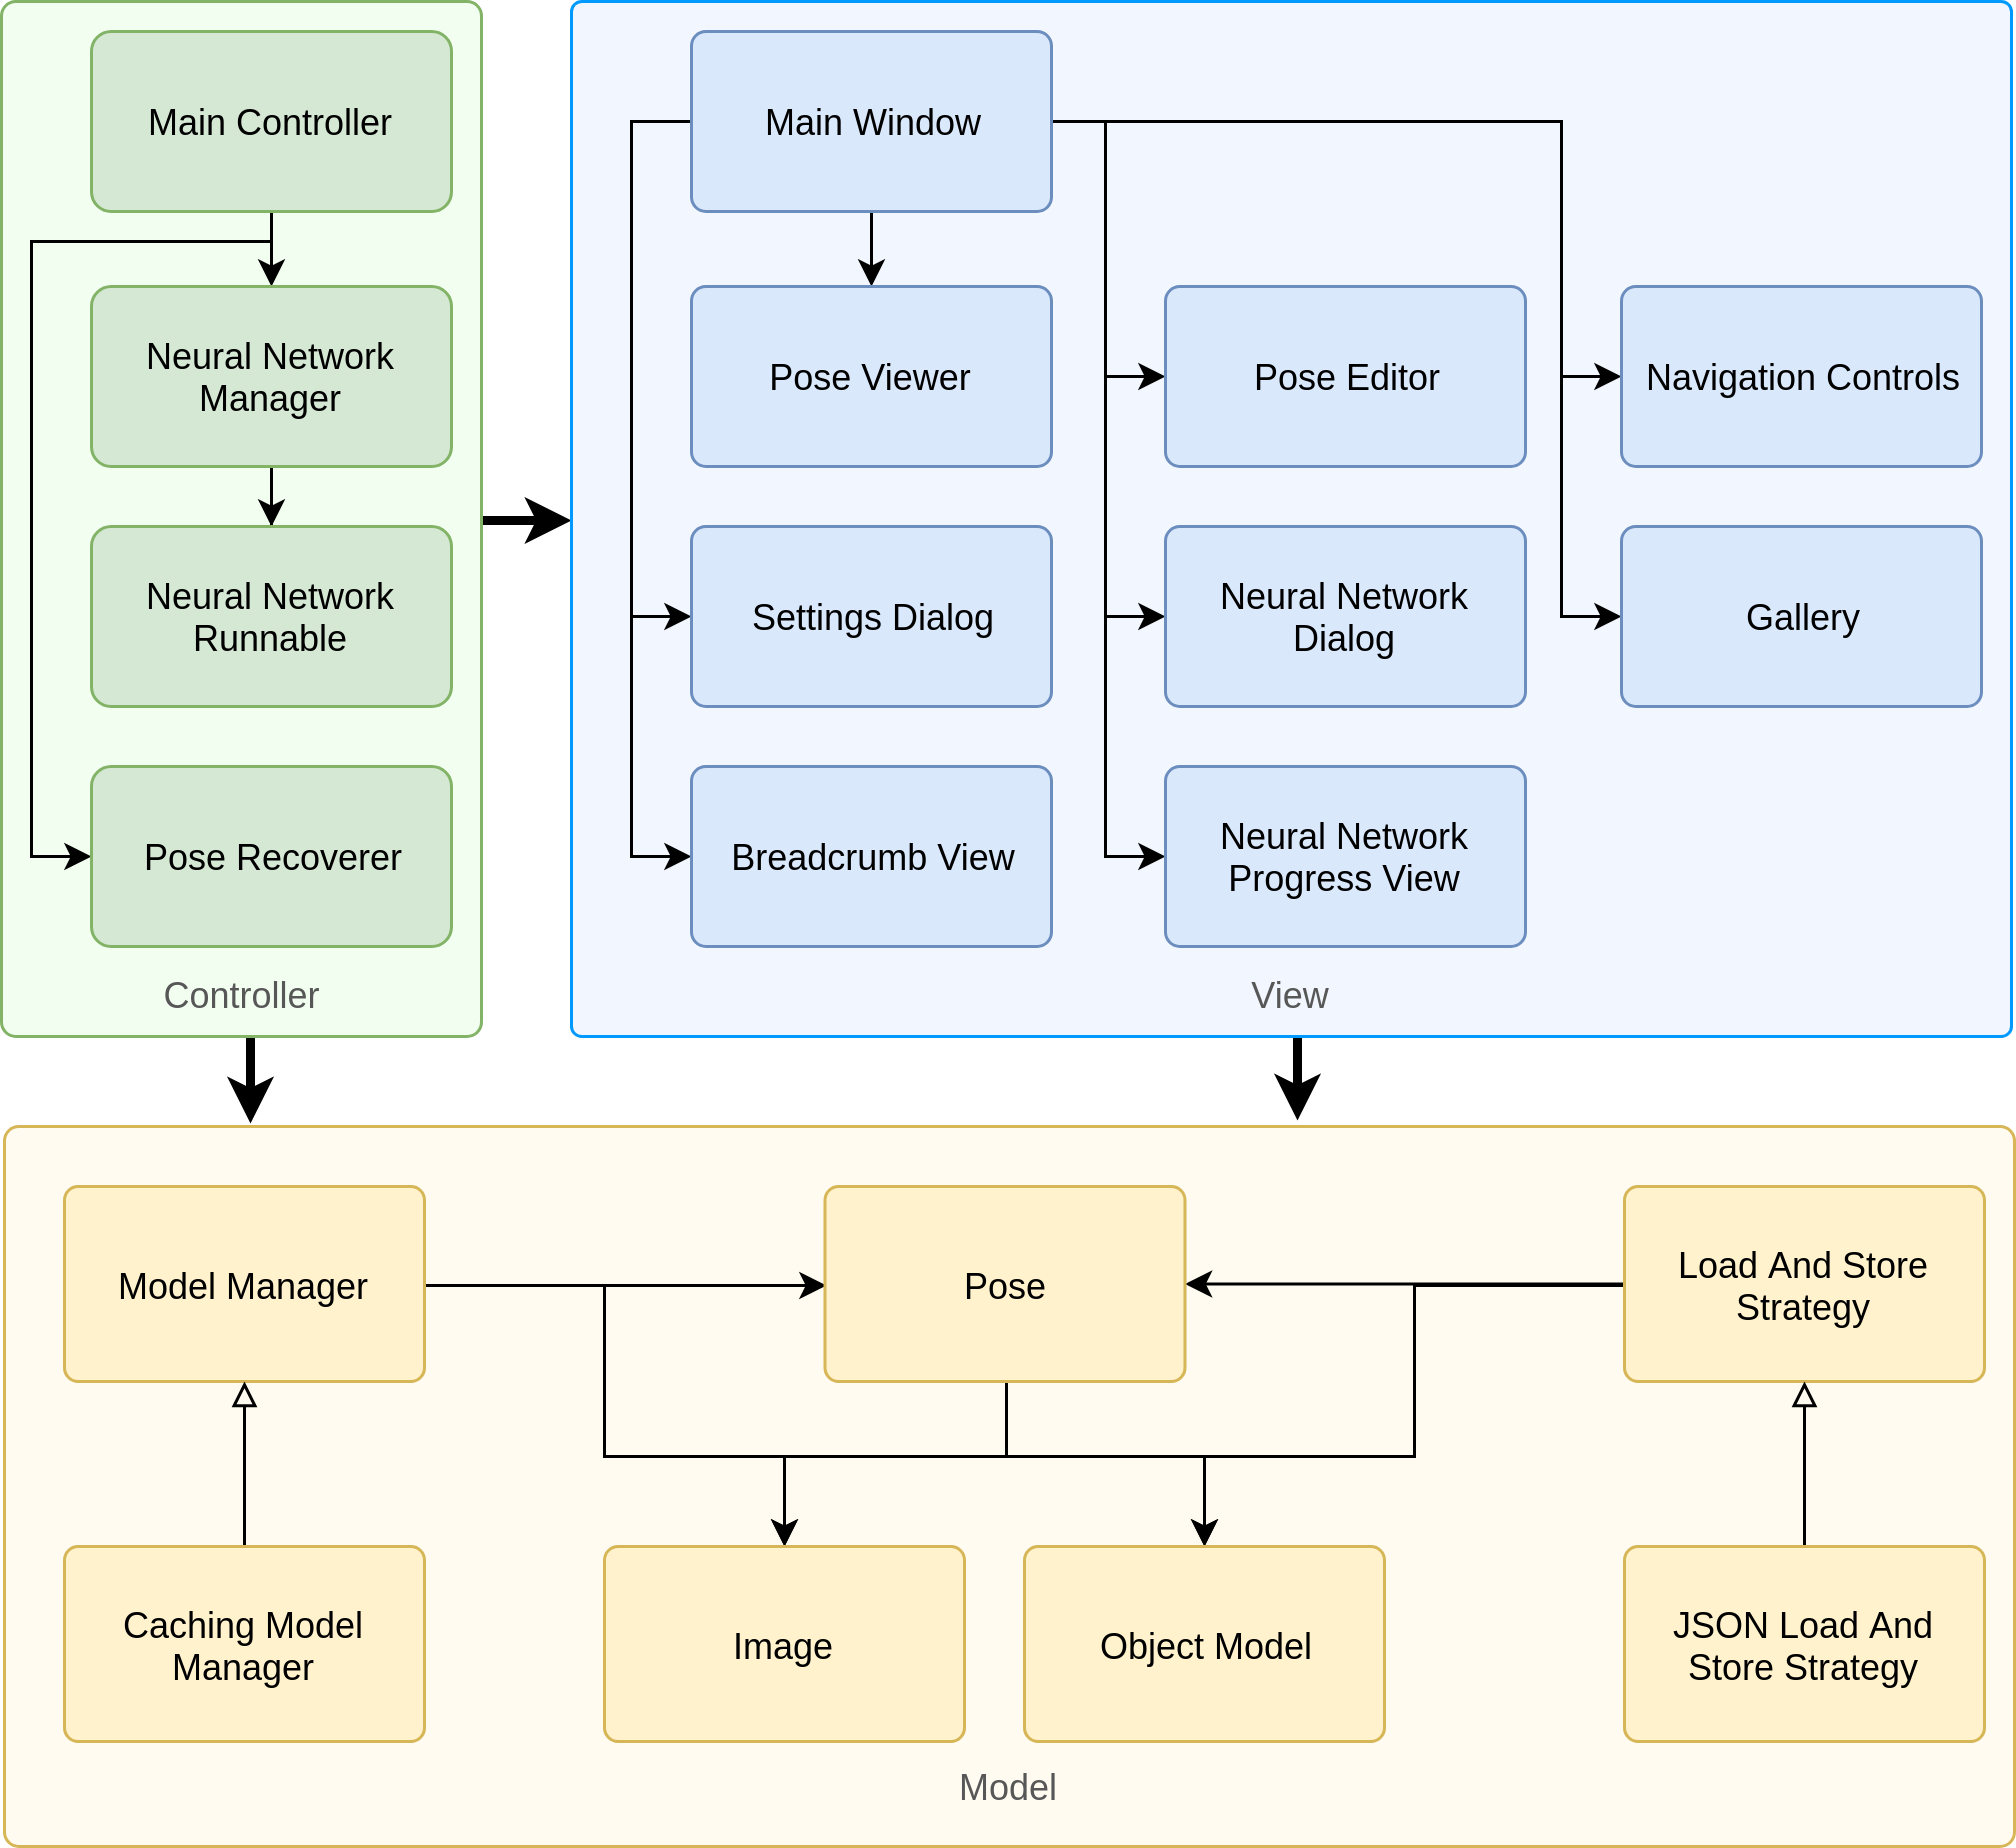
\includegraphics[width=0.9\linewidth]{6dpat_class_diagram}
    \caption{An abstract high-level class diagram of the a subset of the classes of \gls{6dpat}. The thin filled-out arrow-heads mean "uses". The not filled arrow head mean "inherits". Arrows pointing from the larger rectangles imply that the source rectangle uses classes of the target rectangle, although not all classes use all target classes. The \textbf{Main Controller} holds the references to the \textbf{Pose Creator}, the \textbf{Neural Network Manger} and the \textbf{Neural Network Runnable}. The Pose Creator stores the clicked 2D-3D correspondences and implements functionality to recover a pose. The Neural Network Manager controls the connection to the neural network and uses the Neural Network Runnable to execute network tasks. The Main Controller also owns the \textbf{Main Window}, which consists mainly of the classes visible in the "View" rectangle. The \textbf{Pose Viewer} can display images and their poses and the \textbf{Pose Editor} can be used to edit those poses. The \textbf{Settings Dialog} allows editing of several preferences. To let the network predict poses, the user can open the \textbf{Neural Network Dialog} and select images to run prediction on. This opens the \textbf{Neural Network Progress View} until inference has finished. The \textbf{Breadcrumb View} shows the currently set folders to load images and object models from. The \textbf{Navigation Controls} allow navigation through the \textbf{Galleries} showing the images and object models. The \textbf{Model Manager} uses the \textbf{Load And Store Strategy} to load images, object models and poses. The respective classes are depicted in the middle of the large rectangle labeled "Model". The Main Controller owns the Model Manager and passes it to most view classes. Own image.}
    \label{fig:6dpat_class_diagram}
\end{figure} 

\noindent\textbf{Assimp.} \textit{Assimp} \cite{assimp} is a C++ library designed to import 3D models. The library was incorporated into the tool to ensure a broad support of 3D model formats.

\subsection{Architecture \& Code Design}

\gls{6dpat} is primarily a \textit{Graphical User Interface (GUI)} program, i.e. its purpose is to display a window and enable optical interaction like clicking. Thus, the chosen underlying architecture is \textit{Model-View-Controller (\gls{mvc})}, which separates the concerns of data management (Model), displaying data (View) and high level logic (Controller). The schematic of the \gls{mvc} architecture is given in \fig \ref{fig:mvc}. The indirect connections are realized via the Qt Signals and Slots mechanism, which is visualized in \fig \ref{fig:qt_signals_slots}. To speed up interface creation, \textit{Qt Designer} was used to layout the views. Qt Designer is a graphical tool that allows placement of UI components and linking of signals and slots. \\

The most important C++ classes of the program are displayed in \fig \ref{fig:6dpat_class_diagram}. The diagram is simplified for easier understanding. The arrows from the large rectangles imply usage of the classes in the target rectangle. This does not necessarily mean, that all classes of the source use all classes of the target rectangle. The \textit{Pose Editor} uses the \textit{Model Manager} but the \textit{Breadcrumb View} does not, for example. The general structure of the program is the following: the main controller holds references to the \textit{Neural Network Manager}, the \textit{Pose Creator} and the \textit{Main Window}. The neural network manager uses the \textit{Neural Network Runnable} the execute training and inference tasks with the neural network. The pose creator manages the currently clicked corresponding points and computes the new pose when requested and enough corresponding points were clicked. The main window consists of the two main widgets \textit{Pose Editor} and \textit{Pose Viewer}. The pose editor can display an object model $O$ selected from the objects gallery and allows editing all poses $P$ of an image $I$ selected from the images gallery. Both \textit{Gallerys} are owned by the main window, as well. The pose viewer in turn renders all poses $P$ of an image $I$ onto the image. Pose viewer and editor can be used to create new poses (see section \ref{subsection:correspondence_and_pose_creation}). The main window also dispalys the paths selected to load images and object models from using the \textit{Breadcrumb Views}, and allows navigation through the gallerys via the \textit{Navigation Controls}. The settings dialog can be opened from the to edit the preferences of the program. To run the network inference ,the \textit{Neural Network Dialog}, owned by the main window, can be openend to select the images to run prediction on. The main window then displays the \textit{Neural Network Progress View}. Most view classes use the model manager, the \textit{Pose}, the \textit{Object Model} and the \textit{Image} class. Their use should be clear. The main controller sets the \textit{Load And Store Strategy} on the model manager. This class is responsible for reading imags and object models from the hard-drive, as well as persiting poses. The \textit{JSON Load And Store Strategy} uses the JSON format to store poses and read camera matrices. The \textit{Caching Model Manager} is a simple implementation of the model manager interface that chaches images, object models and poses instead of delegating all loading calls to the strategy.

The program expects the camera information and the ground-truth poses file to be in \textit{JSON format}. JSON is a format that is relatively easy for humans to read and is used by many deep learning applications. Transforming JSON formats can be done quickly and therefore provides the possibility to read data from other projects. \\

The program offers functionality to start the network inference. We realized this feature by starting a new process. It is not necessary to use the official C++ Python bridge, offered by the maintainers of Python. The network writes the inferred poses back to a JSON file and we do not need to retrieve any return values directly.

\subsection{Manual Annotation} 

This sections describe the user interface of \gls{6dpat} and the required steps to annotate images with 6D poses. The process needs some actions performed before the actual annotation can be begin. 

\subsubsection{Preparation}

\begin{figure}[!tbp]
	\centering
	\begin{subfigure}[t]{\textwidth}
		\centering
    	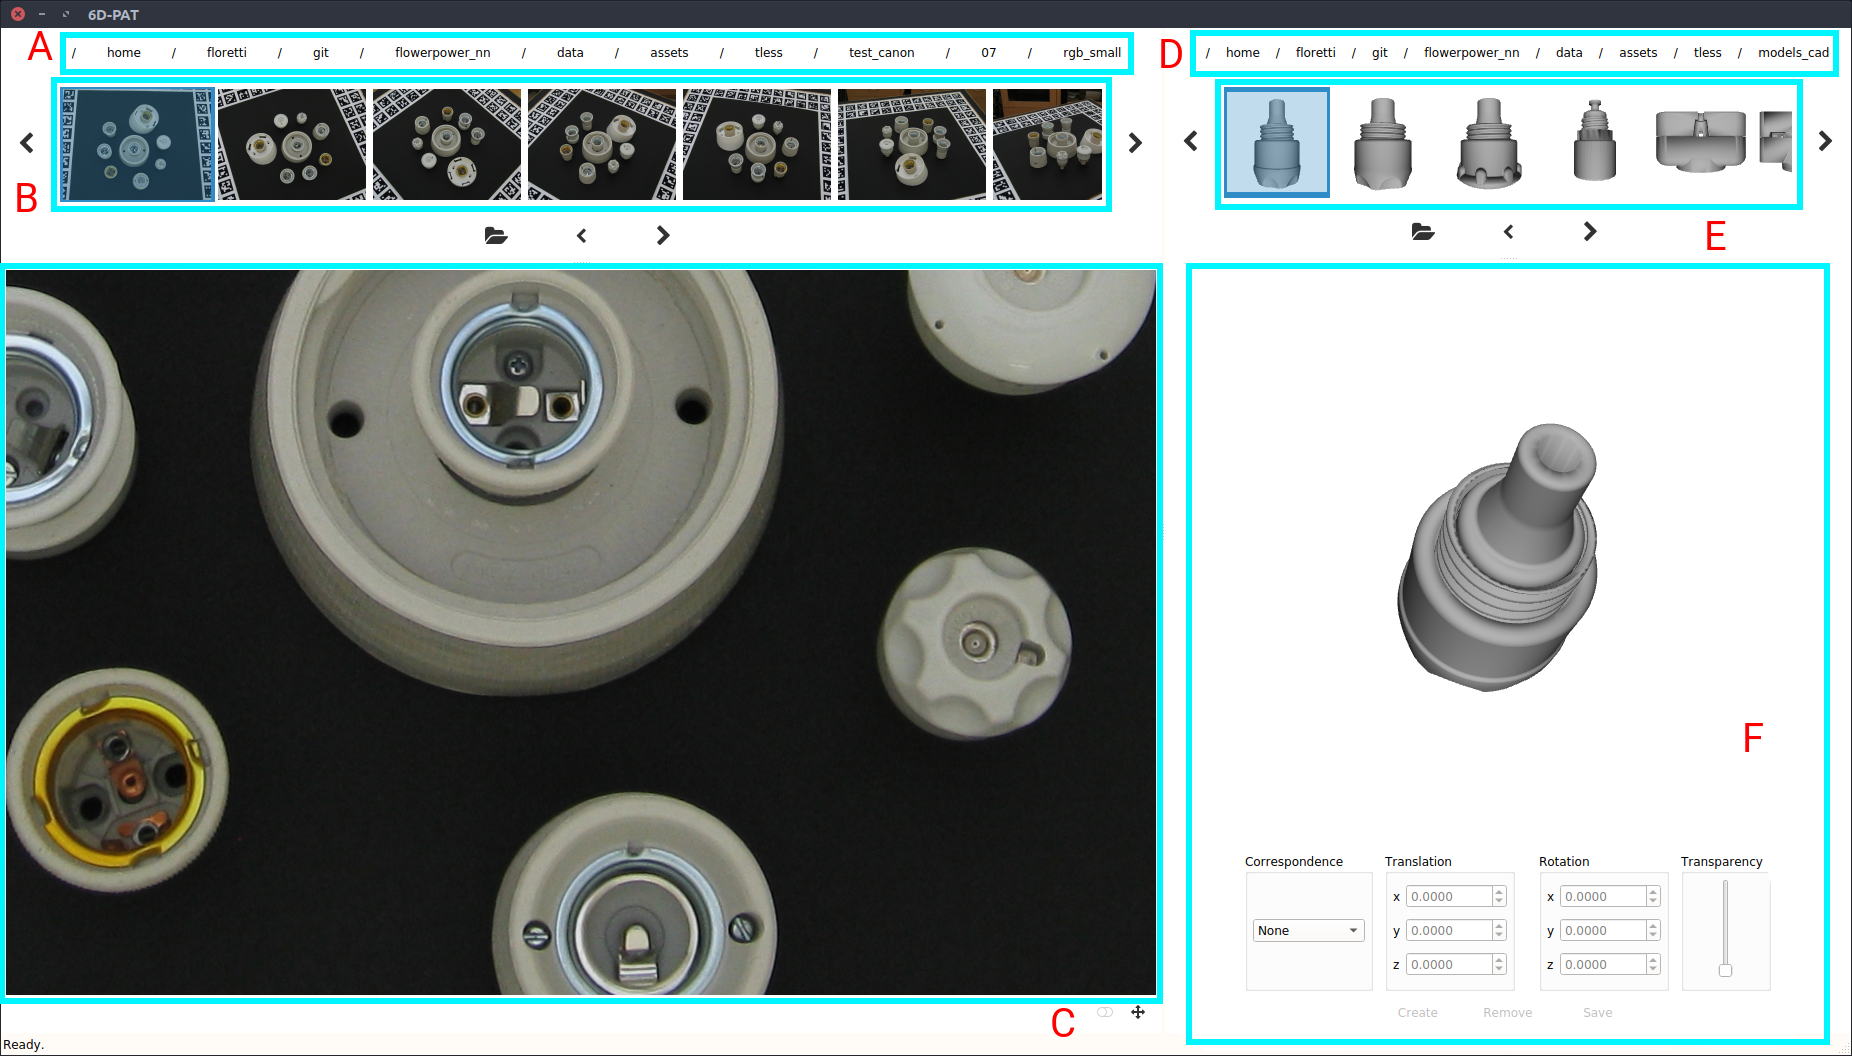
\includegraphics[width=\linewidth]{6dpat_components}
    	\caption{The user interface of the annotation tool \gls{6dpat}. The data displayed are images and object models from the T-Less dataset. The components marked with a turquoise box are the following ones: \textbf{A}: The full path of the currently selected folder to load images from. \textbf{B}: The gallery showing the images loaded from the selected path. \textbf{C}: The \textit{Pose Viewer} shows the image selected in gallery B. The user can click on the image to define the 2D point of a new pose. \textbf{D}: The full path of the currently selected folder to load object models from. \textbf{E}: The rendered 3D preview of the object models loaded from the selected path. \textbf{F}: The \textit{Pose Editor} shows the object model selected in gallery E. The user can click on the object model to complete the correspondence with the 3D point. the controls at the bottom can be used to edit existing poses. Own image.}
    	\label{fig:6dpat_components}
	\end{subfigure}
	\par\bigskip
	\begin{subfigure}[t]{0.47\textwidth}
		\centering
    	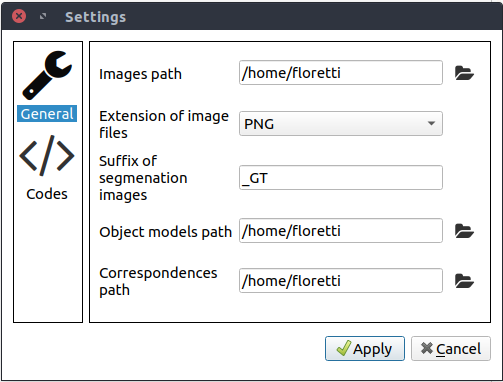
\includegraphics[width=0.8\linewidth]{6dpat_settings}
    	\caption{The settings dialog of \gls{6dpat}. From here the paths to the images and object models can be set, as well as the segmentation image suffix the image type and the file to write the poses to. Own image.}
    	\label{fig:6dpat_settings}
	\end{subfigure}
	\hfill
	\begin{subfigure}[t]{0.47\textwidth}
	\centering
    	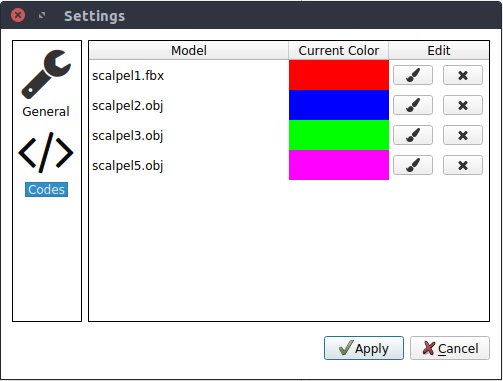
\includegraphics[width=0.8\linewidth]{6dpat_settings_codes}
    	\caption{The settings dialog while editing the colors of the object models in the segmentation images. Own image.}
    	\label{fig:6dpat_settings_codes}
	\end{subfigure}
	\caption{The main view of \gls{6dpat} as well as the two settings views.}
	\label{fig:6dpat_ui_overview}
\end{figure}

The first step after starting the program is to open the settings (see \fig \ref{fig:6dpat_settings}) and set the path to the images that are to be annotated, as well as the path to the folder that contains the object models that should be used for annotation. 

The folder of the images has to contain a JSON file that holds the camera matrix $K$ for each individual image. If no camera info file exists, a Python script, that is distributed with the neural network, can be used to created approximate camera matrices. The path to the segmentation images (if any) has to be set as well. The program loads the images and the segmentation images and sorts them by the numbers in their filenames and then matches image $I$ at index $j$ with the segmentation image $S$ at index $j$. 

Lastly, the location of the JSON file where the ground-truth poses are to be written to has to be specified. If no such file exists an empty one can be created and selected. If segmentation images are present they are linked to the respective image and can be viewed by activating the toggle at the bottom right corner of the pose viewer (the program displaying a segmentation image can be seen in \fig \ref{fig:sfb_segmentation}). 

If required, the colors of the object models in the segmentation images can be set using the settings dialog as shown in \fig \ref{fig:6dpat_settings_codes}. This can reduce the number of displayed tools if many different tools are needed for annotation.

\subsubsection{Correspondence and Pose Creation} \label{subsection:correspondence_and_pose_creation}

The association of letter and component of the annotation tool are visualized in \fig \ref{fig:6dpat_components}. To annotate a new pose an image $I$ has to be selected from gallery \textit{B}, first. The pose viewer \textit{C} then displays the image. The model $O$ that the image is to be annotated with can be selected from the gallery \textit{E}. The pose editor \textit{F} shows the selected object model. The user can rotate the object the reach otherwise hidden areas of it. The arrow keys can be used to move the object along the $x$ and $y$ and also, if the shift key is pressed, along the $z$ axis. 

When the object is in an appropriate position, the user can begin to create a correspondence $C$ by clicking on $I$ and this way defining the 2D point $u$ of the correspondence. To complete the correspondence, the object model $O$ has to be clicked at the respective position $p$. This procedure has to be repeated until enough correspondences have been defined to create the new pose $P$. The minimum is 4 correspondences. 

The creation process is shown in \fig \ref{fig:6dpat_correspondence_creation}. More correspondences can make the initial pose more accurate. Clicking the "Create" button at the bottom of the pose viewer creates the pose $P$ using the correspondences $C_i$ and OpenCV's \textit{solvePnPRansac} method. The newly created pose is directly selected for editing and can be refined using the controls of the pose viewer. After pose refinement it is necessary to click the "Save" button. 

The slider labeled "Transparency" can be used to reduce the object's opacity on the image. After all poses have been annotated successfully the next image can be selected from the gallery B. This operation has to be repeated until the dataset is fully annotated, although intermediate states can be used to train the network already (see chapter \ref{chapter:semi_automatic}).

It is possible to use the neural network to predict poses. This requires a proper setup and training of the network beforehand. The prediction process can be started by clicking the "Predict" button in the lower right corner of the pose editor.

\begin{figure}[!tbp]
	\centering
    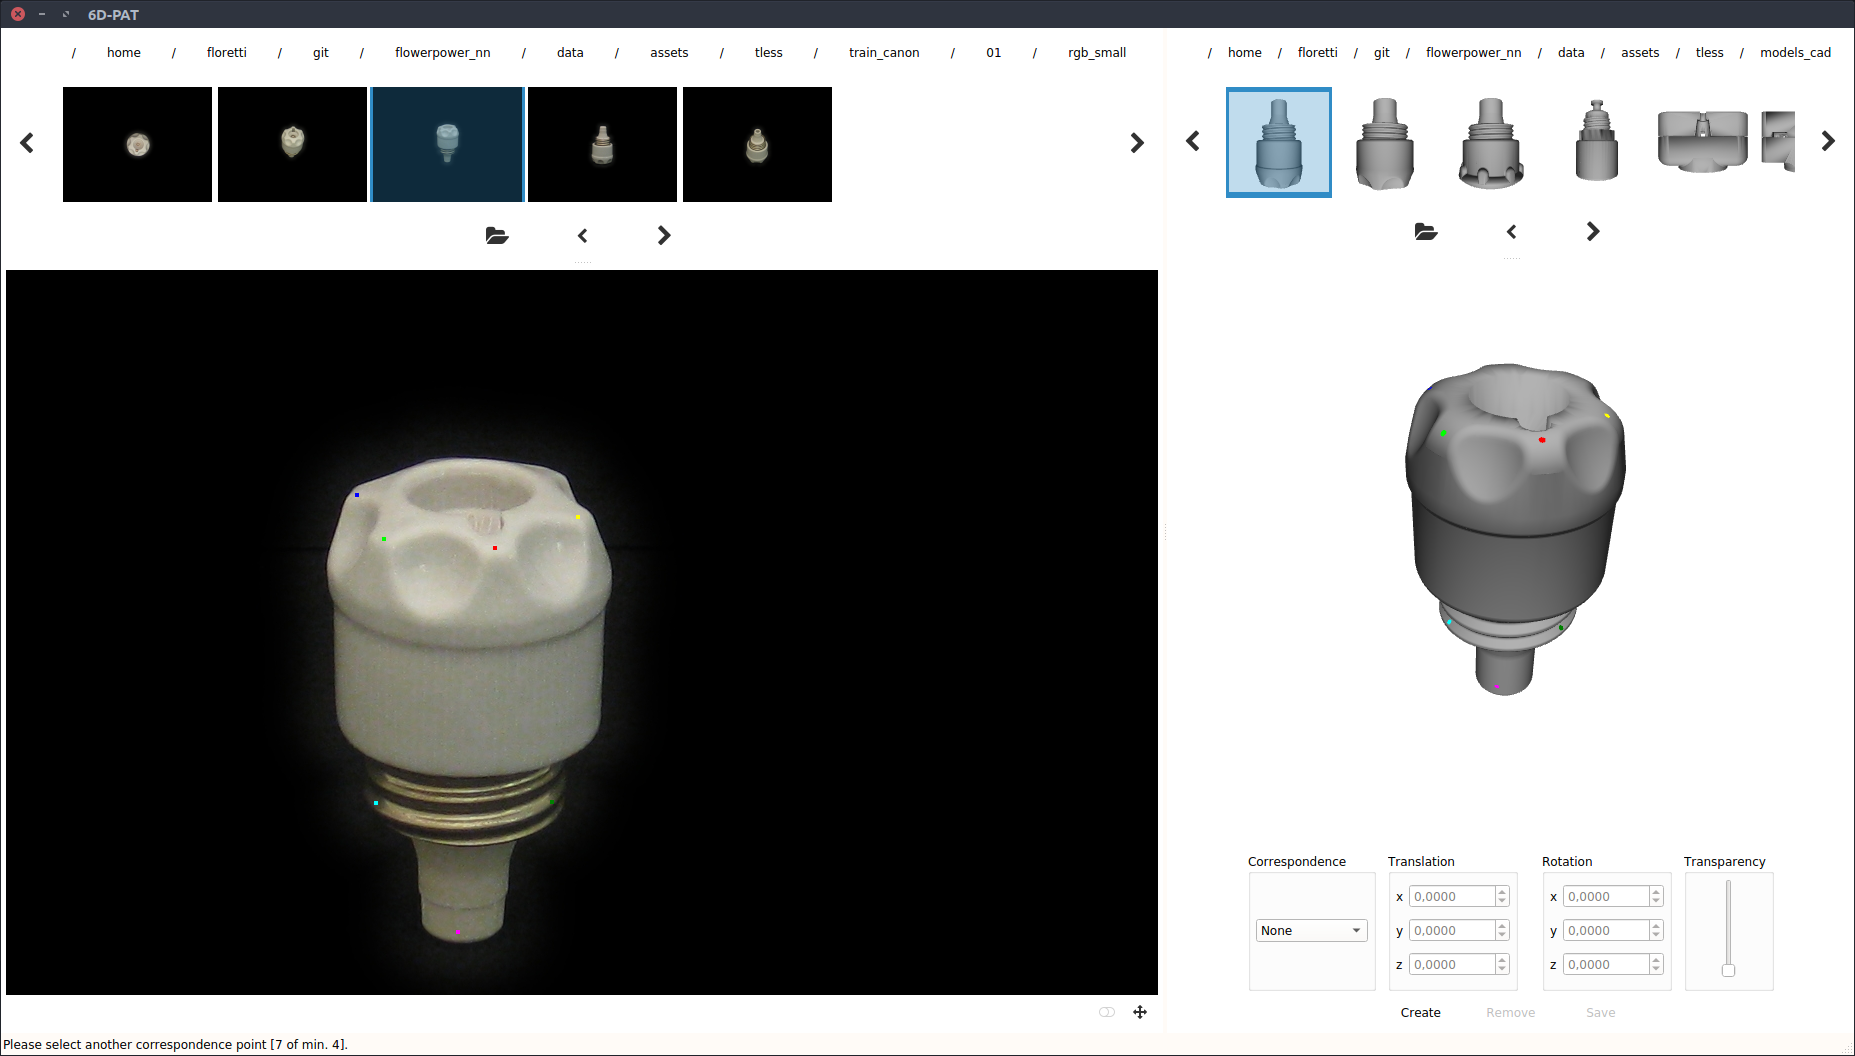
\includegraphics[width=\linewidth]{6dpat_correspondence_creation}
    \caption{The pose creation process. The user has to click the image first and then the corresponding 3D location on the object model. The red circles and red lines were added afterwards to emphasize the colored dots which the program draws. Own image.}
    \label{fig:6dpat_correspondence_creation}
\end{figure} 

\subsection{Problems \& Difficulties} \label{section:6dpat_difficulties}

\begin{figure}[!tbp]
	\begin{subfigure}[t]{0.47\textwidth}
		\centering
    	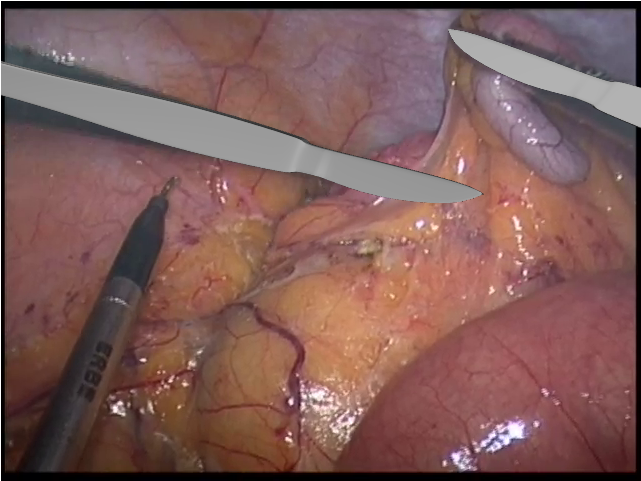
\includegraphics[width=\linewidth]{6dpat_sfb_image}
    	\caption{An image from the medical images dataset annotated using 6D-PAT. The correct rotation and translation are difficult to estimate without the actually used tools. Own image.}
    	\label{fig:6dpat_sfb_image}
	\end{subfigure} 
	\hfill
	\begin{subfigure}[t]{0.47\textwidth}
		\centering
    	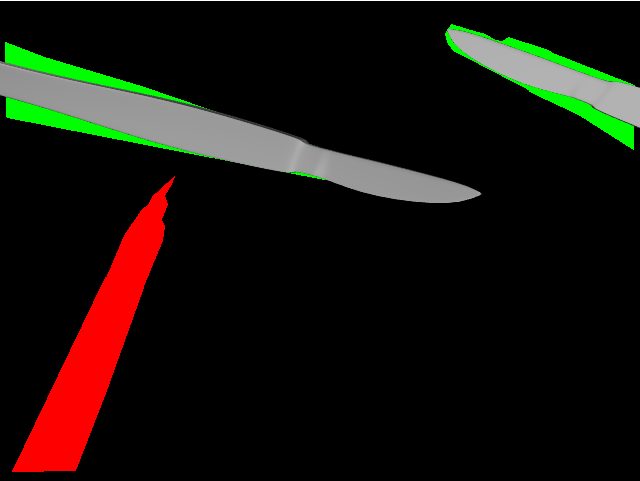
\includegraphics[width=\linewidth]{6dpat_sfb_segmentation}
    	\caption{The corresponding segmentation image to the image on the right. The discrepancy between the segmentation masks and the object model is clearly visible as the green area. Own image.}
    	\label{fig:6dpat_sfb_segmentation}
	\end{subfigure} 
\end{figure} 

During the implementation of the program multiple problems arose and complicated the development process. The most drastic ones are mentioned in this section. Issues contradicting the initial usage patterns and their impact on the final design of the program are explained, as well. \\

One of the major factors that prolong the implementation process was the usage of the only recently released \textit{Qt3D}, which is part of the Qt framework. Qt3D's purpose is to encapsulate graphics programming to increase portability of applications including 3D graphics. The incomplete documentation and unintuitive concepts make it difficult to use without consultation. After more and more complications emerged in the almost completed product the Qt3D framework was deemed unusable and omitted in favor of a native OpenGL implementation. \\

Initially, a desired feature of the program was to present a next unannotated image when the user annotated all poses of an image. This is not feasible for multiple reasons. First of all, a user might still not be content with the poses and might signal that they are finished with the annotation process too early. Thus, it might be disturbing when the program automatically shows the next image. 

The datasets to annotate can also have very distinct characteristics, which require the user to choose the next image personally. For a dataset like T-Less, many images have to be skipped due to their similarity. Intuitively, the more diverse poses are annotated, the better a neural network can be trained. Instead of forcing the user to annotate varying images the motivation should be the sped up annotation process as soon as the neural network is able to make plausible predictions. 

The diversity of kinds of dataset is also the reason why the program does not provide functionality to initialize the next poses based on the ones in the last image. This feature would imply too many assumptions on the dataset and, in the worst case, cause more work for the user. \\

While trying to annotate the medical images dataset it became clear, that proper 3D models are crucial for successful annotation. To temporarily annotate the medical images, 3D surgical tools were downloaded from the internet as a replacement for the missing object models. But having a different shape and also missing the distinctive features of the real objects makes in very difficult to estimate the ground-truth pose. 

The influence of contradicting annotated poses during training of a network is not clear. The author of this work strongly recommends to obtain the correct 3D models before annotating the medical images. The issue of the object models not fitting the segmentation mask can be seen in \fig \ref{fig:sfb_segmentation}. \fig \ref{fig:sfb_original} shows the actual image and the discrepancy between the models and the pixels belonging to the models.

A first try to use the official Python bindings did not work to our complete satisfaction. The rather involved alterations to the program to be able to handle the Python script running inference are too complex compared to starting an external process. Qt offers this functionality already.

The Python binding is not complete yet. Training is not possible and the a deep learning expert has to setup the network and its parameters to enable its usage in the program. The current state of the incorporation of the network is to be seen as a proof of concept that requires further development.

Because the neural network is trained only for one object, the time-intensive step (proportional to the overall time needed for inference on one image) of loading the trained weights has to be performed each time when running inference for different objects. The frame of this work was to explore neural networks trained for one object only.

%%%%%%%%%%% TODO: Evaluation














% Time per annotation etc

T-Less Test images:

0000.jpg 2:30min

0150.jpg 1:23min

0250.jpg: 2:05min

0350.jpg: 3:06min

0500.jpg: 0:50min












%%%%%%%%%%% TODO: Evaluation

\subsection{Future Improvements of \gls{6dpat}}

To provide an outlook how the program can be improved in the future, some key problems as well as their solutions are mentioned here. An important feature that should be implemented is moving the object models around on the displayed image by dragging them. It should also be possible to rotate them with the mouse. The initial poses of the models using the clicking procedure are pretty accurate in many cases already. But sometimes, when the camera is looking along an axis of the object directly, it happens that the rotation is far off. The user can correct the poses with the provided controls. But using them takes some skill and time. The described editing process would profit in terms of time needed per annotation. To give the user a better overview over the image and its annotated poses, a zoom option should be implemented, as well.

The problem of the time needed for loading the weights of the neural network could be solved by offering an intermediate screen that allows to select many images and the object that is to be annotated. The time of loading the weights gets amortized when running inference for many images. 

Another suggested step is to fully incorporate the network in the annotation tool. This way inexperienced users can profit from the network without the need for an expert every time they want it to detect poses in an image. There is probably no way to automatize setting up the network as this requires knowledge of neural nets. In an ideal setting it can be kept to a minimum and users can be introduced to the most relevant parameters, which they can set from within the program.
\chapter{Semi-Automatic Annotation} \label{chapter:semi_automatic}

\begin{figure}[!tbp]
	\centering
    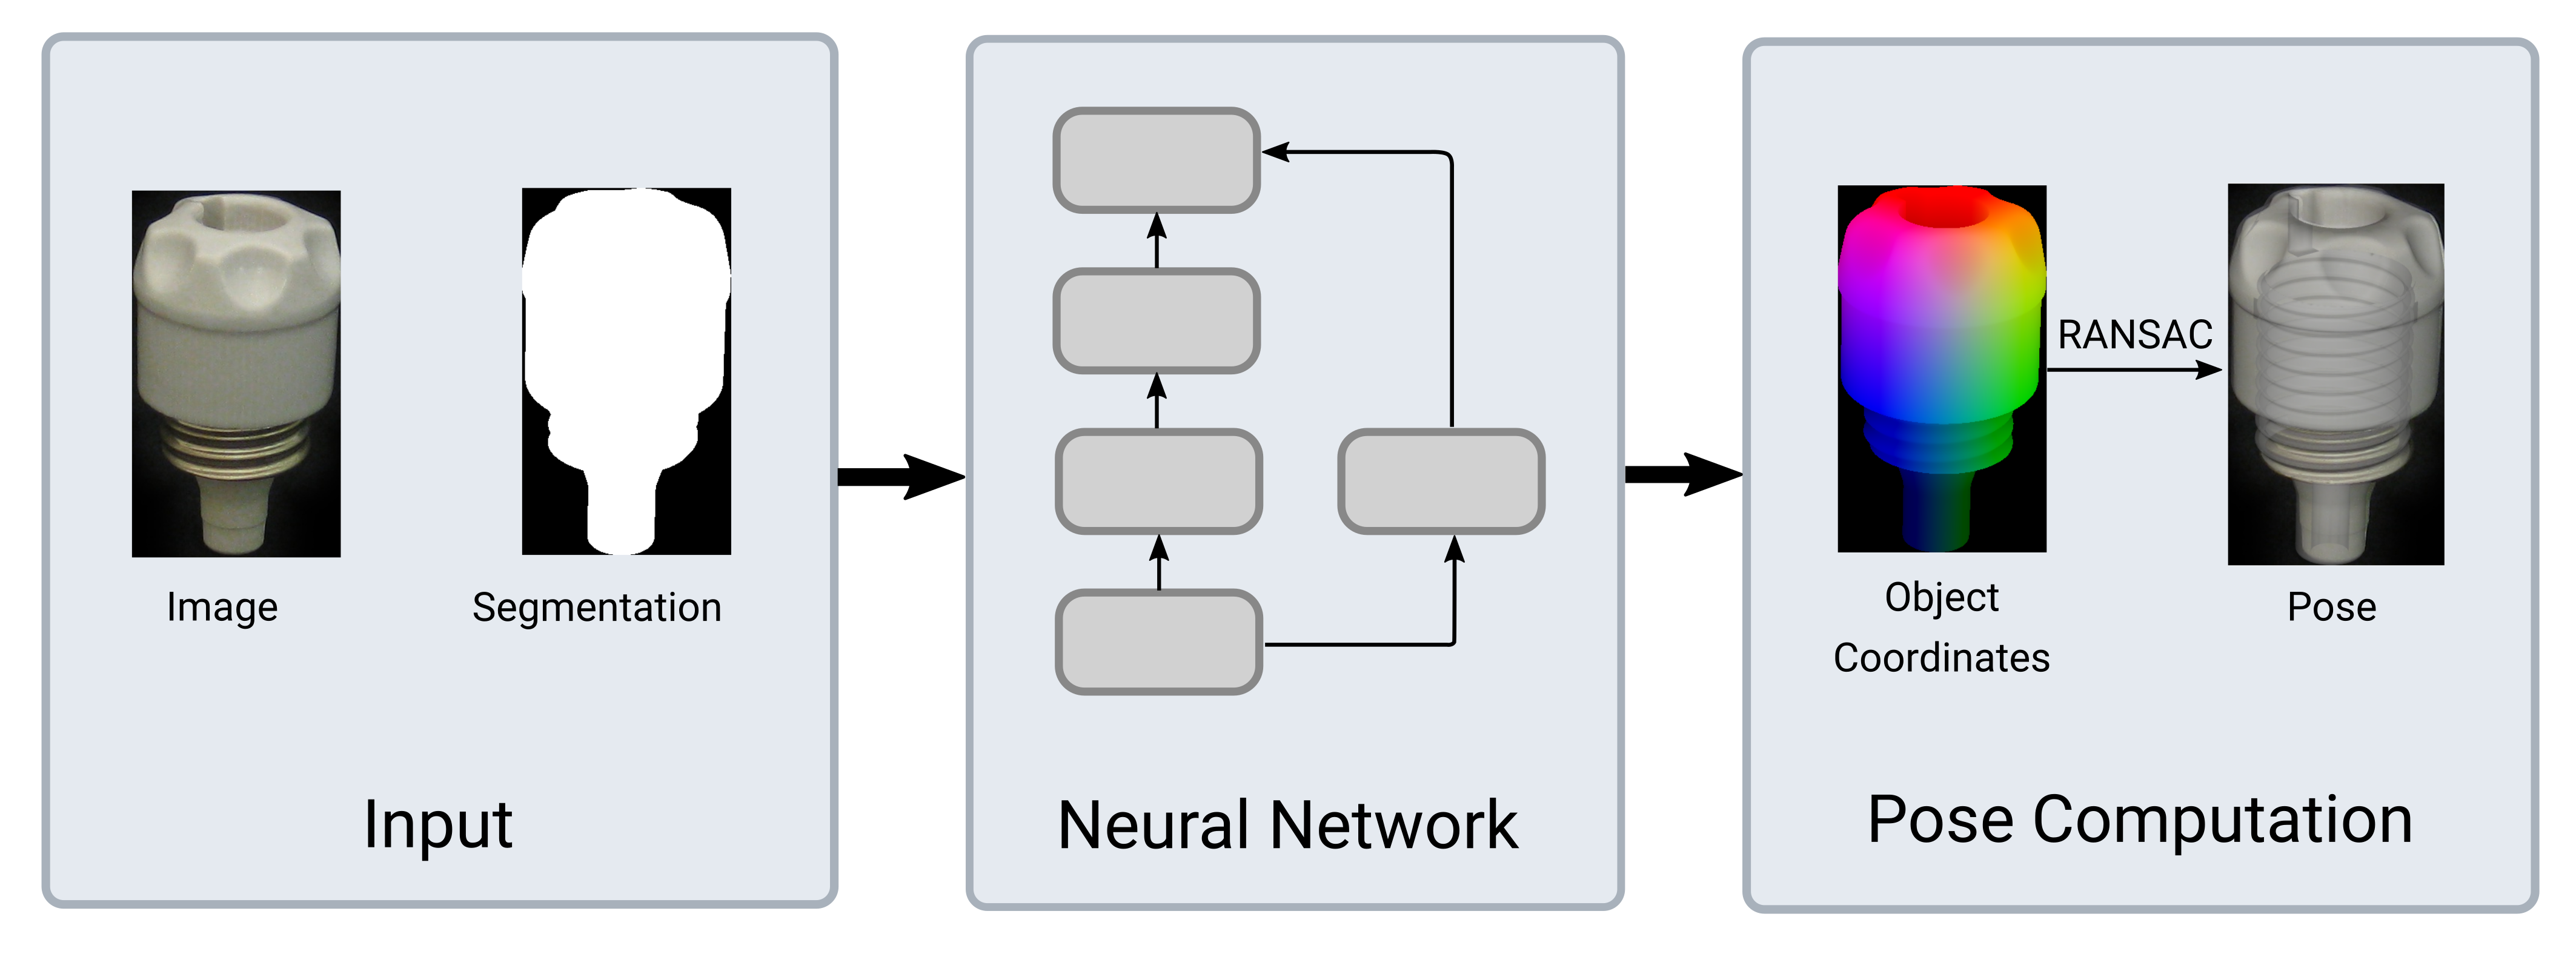
\includegraphics[width=\linewidth]{network_pipeline}
    \caption{The pipeline of the neural network. The two inputs of the network are the image and the corresponding segmentation image. The neural network then uses the segmentation to retrieve the pixels to predict object coordinates for. In the final pose computation stage the object coordinates and their 2D locations are used to retrieve the best pose using \ac{ransac}.}
    	\label{fig:network_pipeline}
\end{figure} 

To assist in the process of manual image annotation presented in Chapter \ref{chapter:manual_annotation}, we developed a neural network for the task of 6D pose estimation tailored to the characteristics of the images of the Endoscopic Vision Challenge. This chapter describes the network architecture and its variations, as well as different approaches to train the network and the resulting modified annotation procedure.

\section{Terminology} \label{section:network_terminology}

\noindent\textbf{Residual Connection.} A \textit{residual connection} (or \textit{skip connection}) is a part of a neural network that skips some layers of the network and adds the input of a layer to the output of a layer that is situated deeper in the network. They can prevent the problem of the increasing training error in deeper networks \cite{resnet}. Fig. \ref{fig:residual_connection} visualizes such a connection. \\

\noindent\textbf{Training Set.} A \textit{training set} is a subset of the dataset intended to train a neural network with. The network uses the training set to adjust its weights as opposed to the validation set. \\

\noindent\textbf{Training Example.} A \textit{training example} is an element from the training set fed to the neural network during training. \\

\noindent\textbf{Training Batch.} A \textit{training batch} consists of a subset of training examples. During training the network updates its weights using all examples in the batch. \\

\noindent\textbf{Validation Set.} A \textit{validation set} is a subset of the dataset intended to train a neural network with. The validation set's purpose is to validate the network's new configuration which emerged from a run within the training. \\

\noindent\textbf{L1 Loss.} The \textit{L1 loss} is a loss function that sums up the results of the function $g$ applied to the $k$ elements in a training batch, i.e. $L_1(x, y) = \frac{1}{k} \sum\limits_k |g(x_k, y_k)|$. We set $g$ to be the euclidean distance: $g(x_k, y_k) = \sqrt{\sum\limits_i (x_{ki} - y_{ki})^2}$, $x_{ki}$ and $y_{ki}$ being the $i$-th entries of the vectors $x_k$ and $y_k$. \\

\noindent\textbf{L2 Loss.} The \textit{L2 loss} is a loss function defined similarly to the L1 loss but sums up the squared instead of the absolute results of $g$, i.e. $L_2(x, y) = \frac{1}{k} \sum\limits_k g(x_k, y_k)^2$. \\

\noindent\textbf{L2 Regularization.} \textit{L2 regularization} penalizes the weights by a factor $\lambda$ in the following way: $\lambda \sum\limits_i w_i^2$. The regularization term is added to the weight update to keep the network from overfitting. \\

\noindent\textbf{Error.} The term \textit{error} denotes the value computed using the loss function. It is essentially the discrepancy between the desired output and the output of the network. It is also called \textit{error rate} or \textit{loss} or, when the loss is computed only on the training data, \textit{training error} or \textit{validation error}, when computed on the validation set. \\

\noindent\textbf{Performance.} The term \textit{performance} denotes the network's accuracy in this work. \\

\noindent\textbf{Dropout Percentage.} \textit{Dropout percentage} is the percentage of neurons to deactivate in a layer during training. \\

\noindent\textbf{Receptive Field-Size.} The \textit{receptive field-size} of a network denotes how many input pixels an output value of the network has taken into account. This factor is determined by the number of operations in the network and their parameters. A convolution operation can skip pixels, which results in a larger receptive field-size. Increasing the kernel size has the same effect. Depending on the field of application a field-size should be larger or smaller.

\section{Frameworks}

The neural network and all of its functionality is implemented in Python using Tensorflow \cite{tensorflow} and Keras \cite{keras}. Tensorflow is a deep-learning framework that uses C++ to perform the actual calculations. It provides many different types of network layers, as well as tools to modify images, automatic differentiation of the loss function and optimization algorithms. Keras is a framework that makes using Tensorflow easier and allows to create neural networks in a few lines of code. Most of the operations of Tensorflow and Keras are performed in C++ but both can be easily used from Python. Both fromeworks offer functionality to transfer the computations to the graphics cards. This allows training deep networks in a feasible time \cite{ylecun}.

\begin{figure}[!tbp]
	\centering
	\begin{subfigure}[t]{0.47\textwidth}
		\centering
    	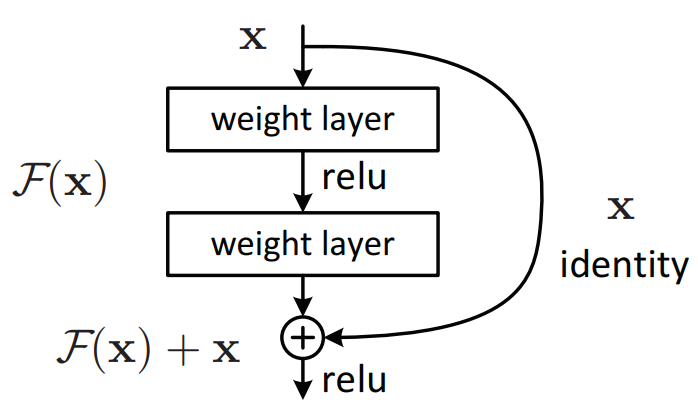
\includegraphics[width=\linewidth]{residual_connection}
    	\caption{A detailed view on a residual connection. The residual connections add the input of earlier layers of the network to deeper ones.}
    	\label{fig:residual_connection}
	\end{subfigure}
	\hfill
	\begin{subfigure}[t]{0.47\textwidth}
		\centering
    	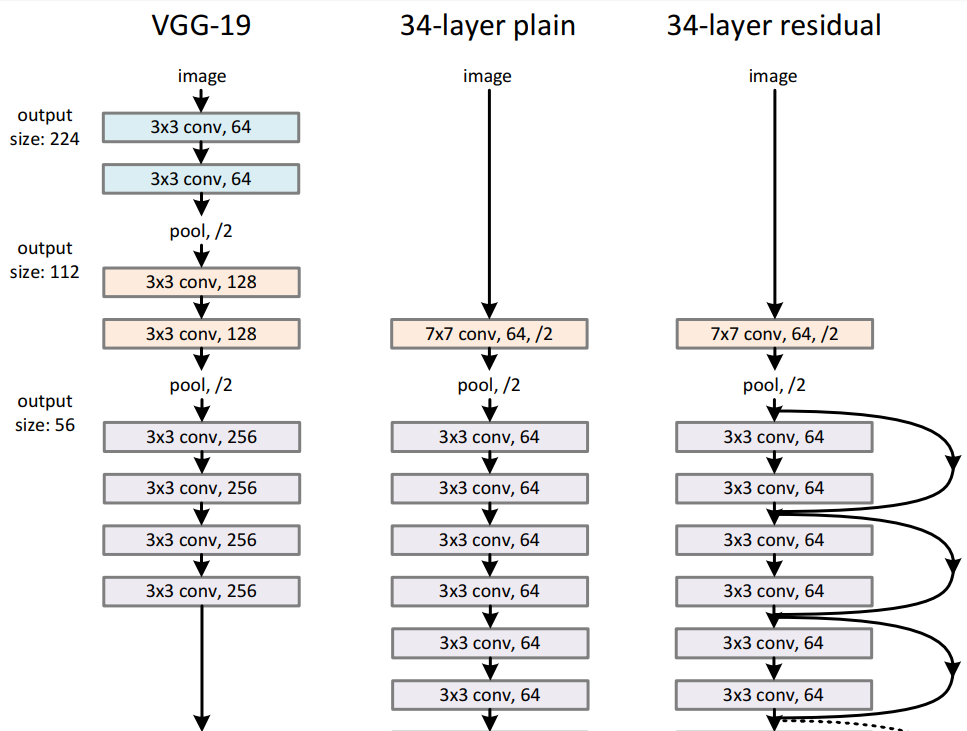
\includegraphics[width=\linewidth]{resnet_comparison}
    	\caption{Excerpt of a comparison between the ResNet architecture and VGG. ResNet allows the creation of deeper network, as the problem of vanishing gradients can be targeted this way. The image has been cropped.}
    	\label{fig:resnet_comparison}
	\end{subfigure}
	\caption{A key component of ResNet: the residual connection. The left image shows the connection in detail and the right image shows a comparison with the VGG architecture. Images from \cite{resnet}.}
	\label{fig:resnet_details}
\end{figure} 

\section{Network Architecture}

The architecture of the network is adjusted to the problem domain of the images of the Endoscopic Vision Challenge. There is no mechanism of inferring the masks and the network expects RGB-only images without depth information. This significantly reduces the complexity of predicting the position of the object. Many contradicting predicted object coordinates can still lead to positional errors, though. \fig \ref{fig:network_pipeline} shows the processing pipeline of the network which takes the image and the segmentation image as inputs. The network processes each pixel which is part of the object according to the segmentation image and outputs the 3D coordinates. As explained in Chapter \ref{chapter:background}, we then compute the optimal pose using RANSAC and the 2D-3D correspondences.

The basic architecture that we chose for the network is called ResNet. He \etal first presented ResNet in 2015, which enabled researchers to create deeper networks than before \cite{resnet}. Two major problems arise in very deep neural networks. One is the vanishing gradients problem, which means that gradients gradually become 0 in deeper layers. A 0-gradient implies that the weights don't change anymore and the layer can't take in the information of the training examples. This problem can be targeted with batch normalization \cite{resnet}. The second problem is that making a network deeper without further adjustments can lead to an increasing training error. Adding layers to a network to increase expressivity does not directly lead to a higher accuracy. Even stacking identity layers, i.e. layers that learn the mathmatical identity function $f(x) = x$, on top of the network increases the training error. This phenomenom can be compensated with residual connections \cite{resnet}. An example of a residual connection can be seen in \fig \ref{fig:residual_connection}. Fig. \ref{fig:resnet_comparison} shows a comparison of ResNet with the architecture \textit{VGG} \cite{vgg}, which is another well known neural network design. The residual connections are clearly visible as the arcs of the rightmost architecture.

We chose ResNet over other architectures due to its easy scalability and its still superior performance in terms of accuracy. \textit{Mask RCNN} is a prominent example that makes use of ResNet's structure \cite{mask_rcnn}. The Facebook AI Research team developed Mask RCNN. The network is still ranking within the top 5 networks of the MS COCO challenge, as of July 2018. The MS COCO challenge is a challenge on image segmentation and object detection \cite{mscoco}.

\begin{figure}[!tbp]
	\centering
    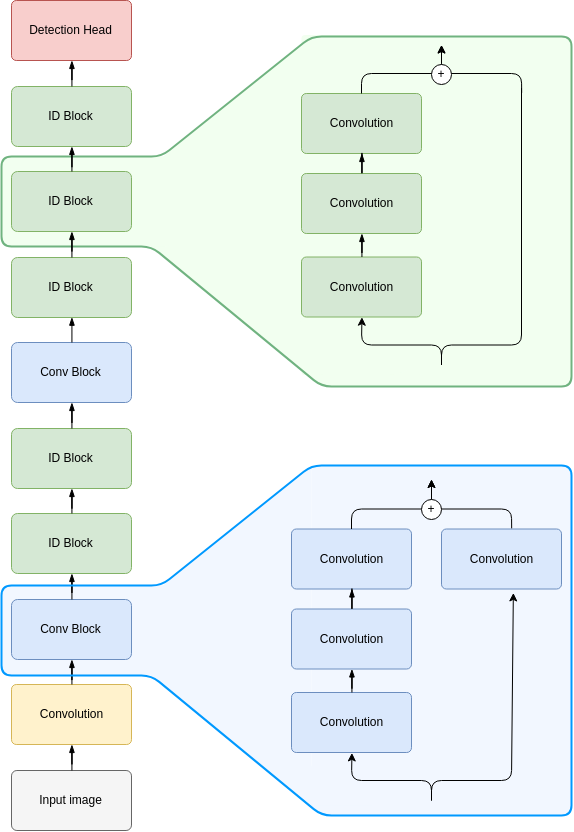
\includegraphics[width=0.9\linewidth]{flowerpower_short}
    \caption{Architecture 1 with a total of 23 (convolutional) layers. The components of the \textbf{Conv Block} and \textbf{ID Block} elements are visualized on the right. The characteristic of the Conv Block is that it applies a convolution on the shortcut connection while the ID Block doesn't. The yellow \textbf{Convolution} rectangle is a plain convolution layer. The \textbf{Network Head} consists of another three convolution layers.}
    	\label{fig:network_architecture}
\end{figure}

The structure of the network is visualized in \fig \ref{fig:network_architecture}. The depicted architecture has 23 convolutional layers (see Section \ref{section:network_variations} for a detailed explanation on used architecture variations). The building blocks of the network are the \textit{Conv Block} and the \textit{ID Block}. Both blocks are shown in detail on the right. A Conv Block applies another convolution to the shortcut connection on the right and then combines the result with the output of the left path. The ID Block simply adds the input to the result of the convolutions on the left. The figure doesn't show the batch normalization and \textit{activation layers} to keep the illustration clear. The actual network has a batch normalization layer followed by an \textit{activation layer} after each convolution layer. Activation layers are layers in Keras that apply a specified activation function to their input. This way, non-linear neurons are realized in the framework. All layers employ the \ac{relu} activation function.

\subsection{Loss Function \& Optimizer}

Since the network outputs the 3D coordinates for each pixel in the input image a straight-forward approach is to penalize the euclidean distance with respect to the ground-truth coordinates. The loss function sums up these distances of the individual $XYZ$ components of the predicted object coordinate and the ground-truth, but only at the relevant positions according to the segmentation mask. This resembles the L1 loss (see Section \ref{section:network_terminology}). The L2 loss potentially penalizes outliers more. But outliers get eliminated in the \ac{ransac} algorithm during pose computation and thus might not have to be taken into account by a great extend. The L2 loss might strive for a worse compromise between outliers and accurate coordinate predictions. To verify our beliefs we compared both loss functions in  Chapter \ref{chapter:experiments}. To find the best optimizers, we also compared SGD and Adam (same chapter).

\subsection{Variations} \label{section:network_variations}

The problem formulation of this work demands exploration of multiple architecture designs. There are multiple reasons why. The Endoscopic Vision Challenge dataset does not provide any pose annotations at all. This means that the user likely trains the neural network with few images at first. 

A very deep network with many layers might not be able to incorporate the little information optimally. Conversely, a shallower architecture might not reach the same performance as a deeper network. 

A characteristic of the Endoscopic Vision Challenge dataset is that the tools have writings on them which are often not or only partly visible. A network with a large receptive field-size could tend to predict 3D coordinates based on this very distinct feature, even for pixels that are further away. This way, less prominent characteristics, that could still be used to accurately identify the object coordinate belonging to a pixel, might be disregarded and the pose correctness might drop when the letters are not visible.

\begin{table}[]
\centering
\begin{tabular}{|l||llllll|}
\hline Architecture No.        & 1          & 2          & 3          & 4          & 5          & 6        \\ \hline\hline
\rowcolor{Gray}
\# Layers               & \textbf{23}         & \textbf{35}         & \textbf{23}         & \textbf{50}         & \textbf{50}         & \textbf{50}       \\
Receptive field-size    & 99         & 67         & 51         & 59         & 59         & 59       \\
\rowcolor{Gray}
\# Parameters & 3,95  & 19,69 & 6,32  & 24,63 & 24,63   & 24,63 \\
Data normalization      & bn & bn & bn & do    & bn & do \\ \hline
\end{tabular}
\caption{Overview over the differences between the network architectures. The number of layers corresponds to the number of convolutional layers. Batch normalization layers are not counted. The abbreviations \textit{bn} and \textit{do} stand for batch normalization and dropout, respectively. The number of parameters is given in millions. The number of parameters resembles the number of trainable variables in the network.}
\label{table:network_architectures}
\end{table}

Employing batch normalization can reduce the training time needed for a network, as well as increase its accuracy \cite{batch_normalization}. To exploit the full potential of batch normalization, a batch has to consist of enough training examples so that the normalization represents a good approximation of the statistics of the dataset. Due to the limited memory resources on graphics cards, a large batch size is not always possible for deep networks because Tensorflow transfers the training examples to the GPU memory for optimal speed. This is the reason why we believed it necessary to compare batch normalization and dropout. These challenges gave rise to the architectures described in the following paragraphs.

We created the initial design of the network with 23 convolutional layers and a receptive field-size of 99. The second architecture consists of 35 layers, while decreasing the receptive field-size to 67. 

The third architecture has the same number of layers like the first architecture but a reduced receptive field-size of 51. Architectures 4 to 6 all have a receptive field-size of 59 and 50 convolutional layers. While architecture 5 uses batch normalization for regularization, architectures 4 and 5 use dropout instead. The difference between those two is the dropout percentage. An overview over the architectures can be seen in Table \ref{table:network_architectures}. 

The number of parameters does not scale linearly with the number of layers, as deeper layers have more filters. The reason why architecture 3 has more trainable parameters than architecture 1 is not entirely clear. The difference between the two networks is that architecture 3 uses a reduced kernel size on deeper layers to obtain a smaller receptive field-size. But this should not cause the number of parameters to grow in a fashion that is visible in the table.

The different depths of the network architectures are visualized in Appendix \ref{appendix:network_architectures}. The architectures that omit the batch normalization layers and employ dropout layers instead are not listed separately, because the number of the convolutional layers is the same as in architecture 5.

\section{Setup \& Implementation Details}

Before the user can run the network to train on a dataset, some steps to setup the network have to be performed. Existing ground-truth files of a dataset have to be converted to the format expected by the network. An example conversion function is provided, which converts the T-Less format to the JSON format that the network is able to read. 

The T-Less dataset does not provide segmentation masks, nor object coordinates. The mask and coordinate images can be rendered using the images, the ground-truth poses file and the utility scripts of the network. After obtaining all data necessary for training, the user needs to write a JSON configuration file, which holds the paths to the data and the parameters of the network. The network architecture that is to be trained can be defined directly in the file. 

The network consists of convolutional, batch normalization and pooling layers only. This means, it can be applied to arbitrary image sizes without having to retrain the network, as in contrast to networks employing fully-connected layers. If the image size changes, a fully-connected layer has to be retrained but a convolutional layer not. The maximum image size needs to be specified in the configuration file, nevertheless. This is necessary because the network is trained in batches instead of single training examples and Keras expects all samples to have the same dimension. The training procedure automatically scales up images smaller than the configured size as much as possible and, for non-square images, pads the remaining space with 0s. It is important to note that during training no cropping of the input data to the relevant area takes place because, to save disk space, we assume the user always crops the training data beforehand. In contrast, the network crops images to the mask area before an inference run. Thus, the data does not need to be altered in any way when only predicting poses.

\section{Modes of Operation} \label{section:modes_of_operation}

The goal of the neural network is to make the annotation process presented in Chapter \ref{chapter:manual_annotation} faster and more efficient. To achieve this, we strove for a symbiosis between the annotation tool and the neural network. The new workflow is visualized in \fig \ref{fig:semi_automatic_workflow}. In addition to manually annotating images, the user can train the network with the annotated data. After training, the neural network can be used to predict poses in previously unseen images. As the network will likely make errors, the poses can be corrected afterwards using \ac{6dpat}. The improved pose predictions can serve as input to further train the network. As the dataset of the Endoscopic Vision Challenge does not provide any pose annotations, the question how to optimally train the network with a reduced set of images arises. The following sections describe different strategies which are evaluated in Chapter \ref{chapter:experiments}.

\begin{figure}[!tbp]
	\centering
    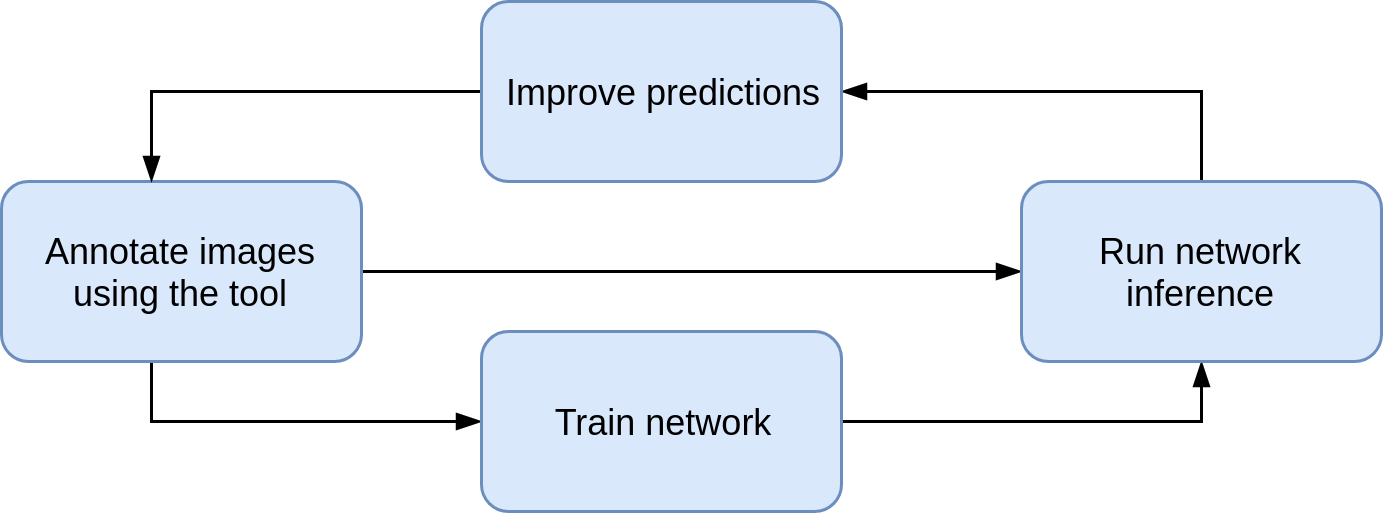
\includegraphics[width=0.75\linewidth]{semi_automatic_workflow}
    \caption{The new workflow of the annotation procedure including the neural network. First, the user has to annotate enough images from the dataset to be able to train the network. After successfully training the network it can be used to predict poses on a subset of the dataset. The user can then improve the poses and return to annotating more images or run the network inference on more images.}
    	\label{fig:semi_automatic_workflow}
\end{figure}

\subsection{Incremental Training} \label{subsection:online_learning}

During the annotation process, the user can train the network using the new data. Given that at the beginning likely no poses exist and the user first has to annotate a couple of images manually, we have to use the little available data as optimally as possible. One option is to fully retrain the network with all  annotated images. This procedure is called \textit{training from scratch}. It is also possible to train the network incrementally, instead. \textit{Incremental training} means that the user trains the network using the annotations that were created after the last training run. In this approach, the weights of the network are not initialized to 0 or randomly. Instead, the weights of the last training run are loaded and trained further using the new data. This method is likely to converge faster and generally needs less time to complete the training compared to training from scratch. We compare the network performance of both approaches in the next chapter.

\subsection{Active Learning} \label{subsection:active_learning}

An intuitive approach to optimally train the network with only a few images is to propose to the user to annotate images which the network does not perform well on. This gives rise to the question how to obtain an indication of the network's accuracy without any ground-truth poses. As the Endoscopic Vision Challenge dataset provides segmentation masks, a simple but direct approach is the compute the intersection over union between the given segmentation mask and a rendered mask using the inferred poses. The intersection over union is defined in the following way
\begin{align*}
\text{IoU} = \frac{\sum\limits_{(i, j)} \mathbbm{1}[s_g(i, j) = q] \cdot  \mathbbm{1}[s_p(i, j) = q]}{\sum\limits_{(i, j)} \frac{\mathbbm{1}[s_g(i, j) = q] +  \mathbbm{1}[s_p(i, j) = q]}{2}}
\end{align*}
where $s_g$ and $s_p$ are the segmentation mappings of the ground-truth segmentation mask and the rendered segmentation mask, respectively (see Section \ref{section:terminology} for details on segmentation masks). $q$ is the type of the object model. $\mathbbm{1}$ is a function that becomes 1, if the statement inside is true, 0 otherwise. Therefore, the formula sums up all pixels that both segmentation masks assign the same type to. It then divides this sum by the whole area covered by this type in both masks. Note that, by dividing the whole area by 2, the $\text{IoU}$ becomes 1 if the masks match exactly. The training process can suggest images to the user that need correction of the recovered poses based on this measure. The next chapter explores this method experimentally.
%TODO provide example ground-truth object coordinates and predictions

\chapter{Experiments} \label{chapter:experiments}

The following section describes the setups of the experiments conducted with the neural network presented in chapter \ref{chapter:semi_automatic}. Due to the lack of existing annotated medical data the focus of the experiments is to ascertain a network design and mode of operation that compensate this as best as possible. First, we test the different network architectures that were described in section \ref{section:network_variations} using the same parameters. We then choose the best architecture for further experiments, in which we evaluate the two different training schemes introduced in section \ref{section:modes_of_operation}: training from scratch and incremental training.

\section{Terminology}

\noindent\textbf{Hyper-Parameter.} \textit{Hyper-parameters} are the tunable parameters of a network. The number and kind of parameters varies with the used type of network architecture, optimizer, etc.

\section{Datasets}

\begin{figure}[!tbp]
	\centering
	\begin{subfigure}[t]{0.47\textwidth}
		\centering
    	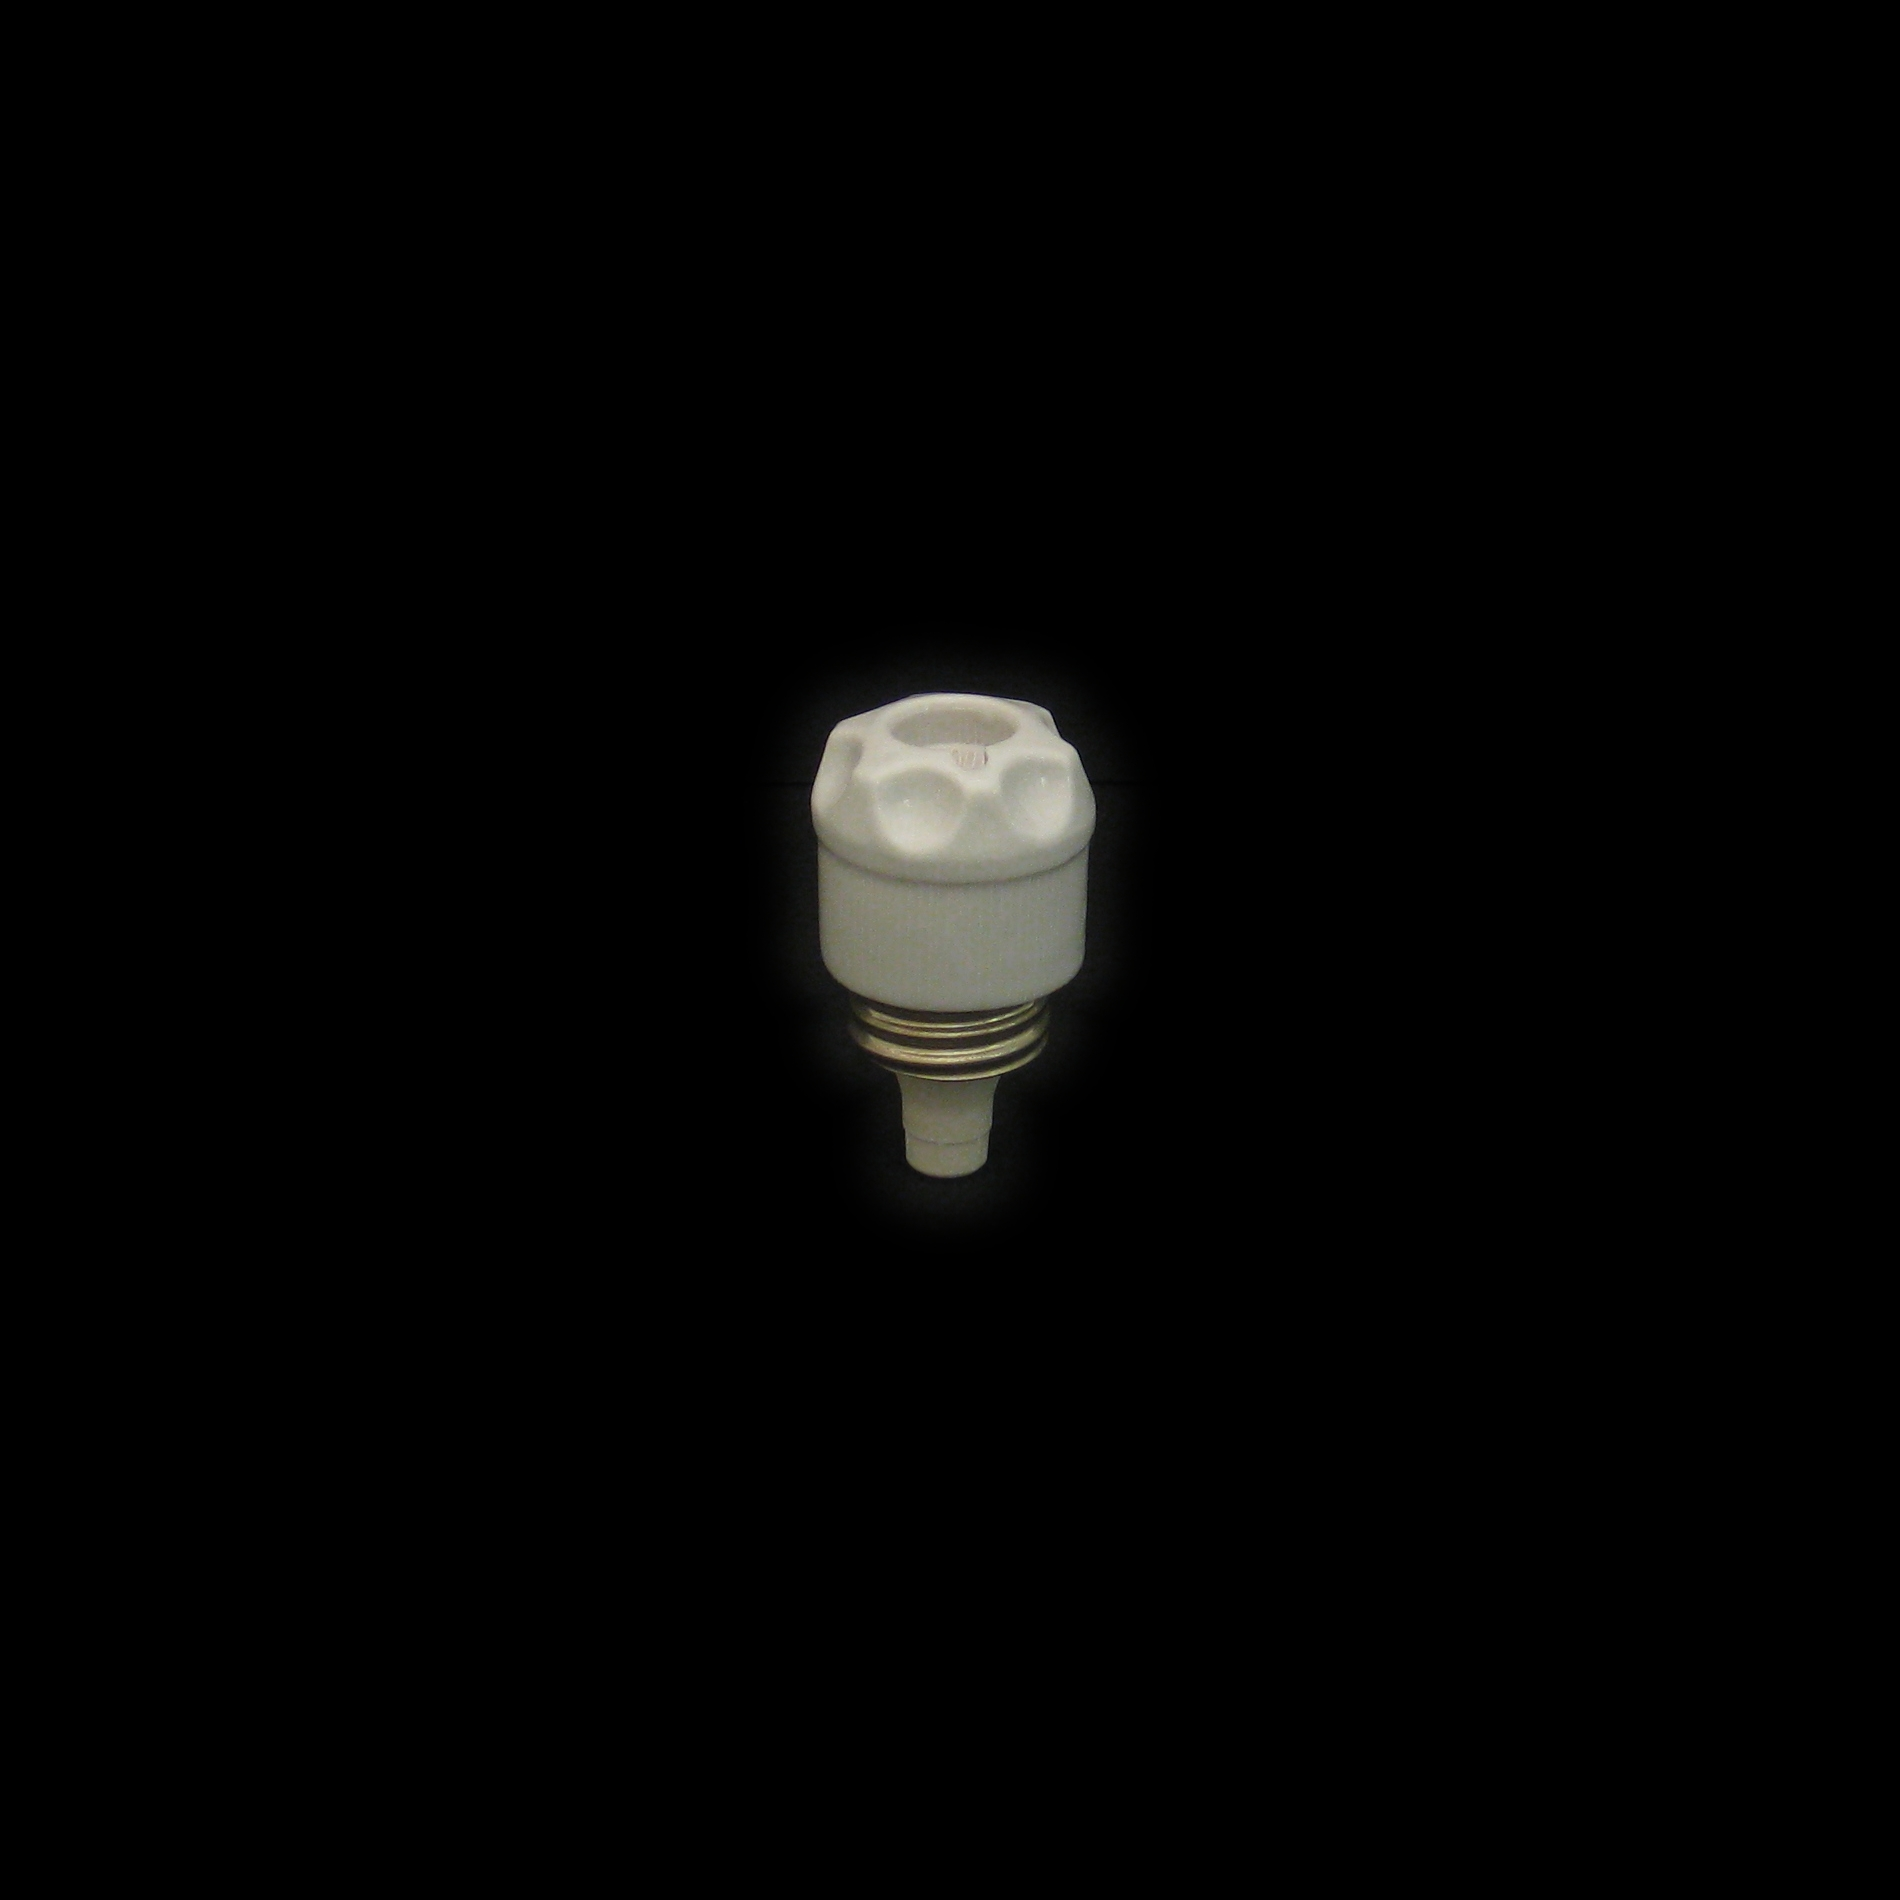
\includegraphics[width=0.6\linewidth]{tless_example_train}
    	\caption{An example frame from the training dataset of T-Less.}
    	\label{fig:tless_example_train}
	\end{subfigure}
	\hfill
	\begin{subfigure}[t]{0.47\textwidth}
		\centering
    	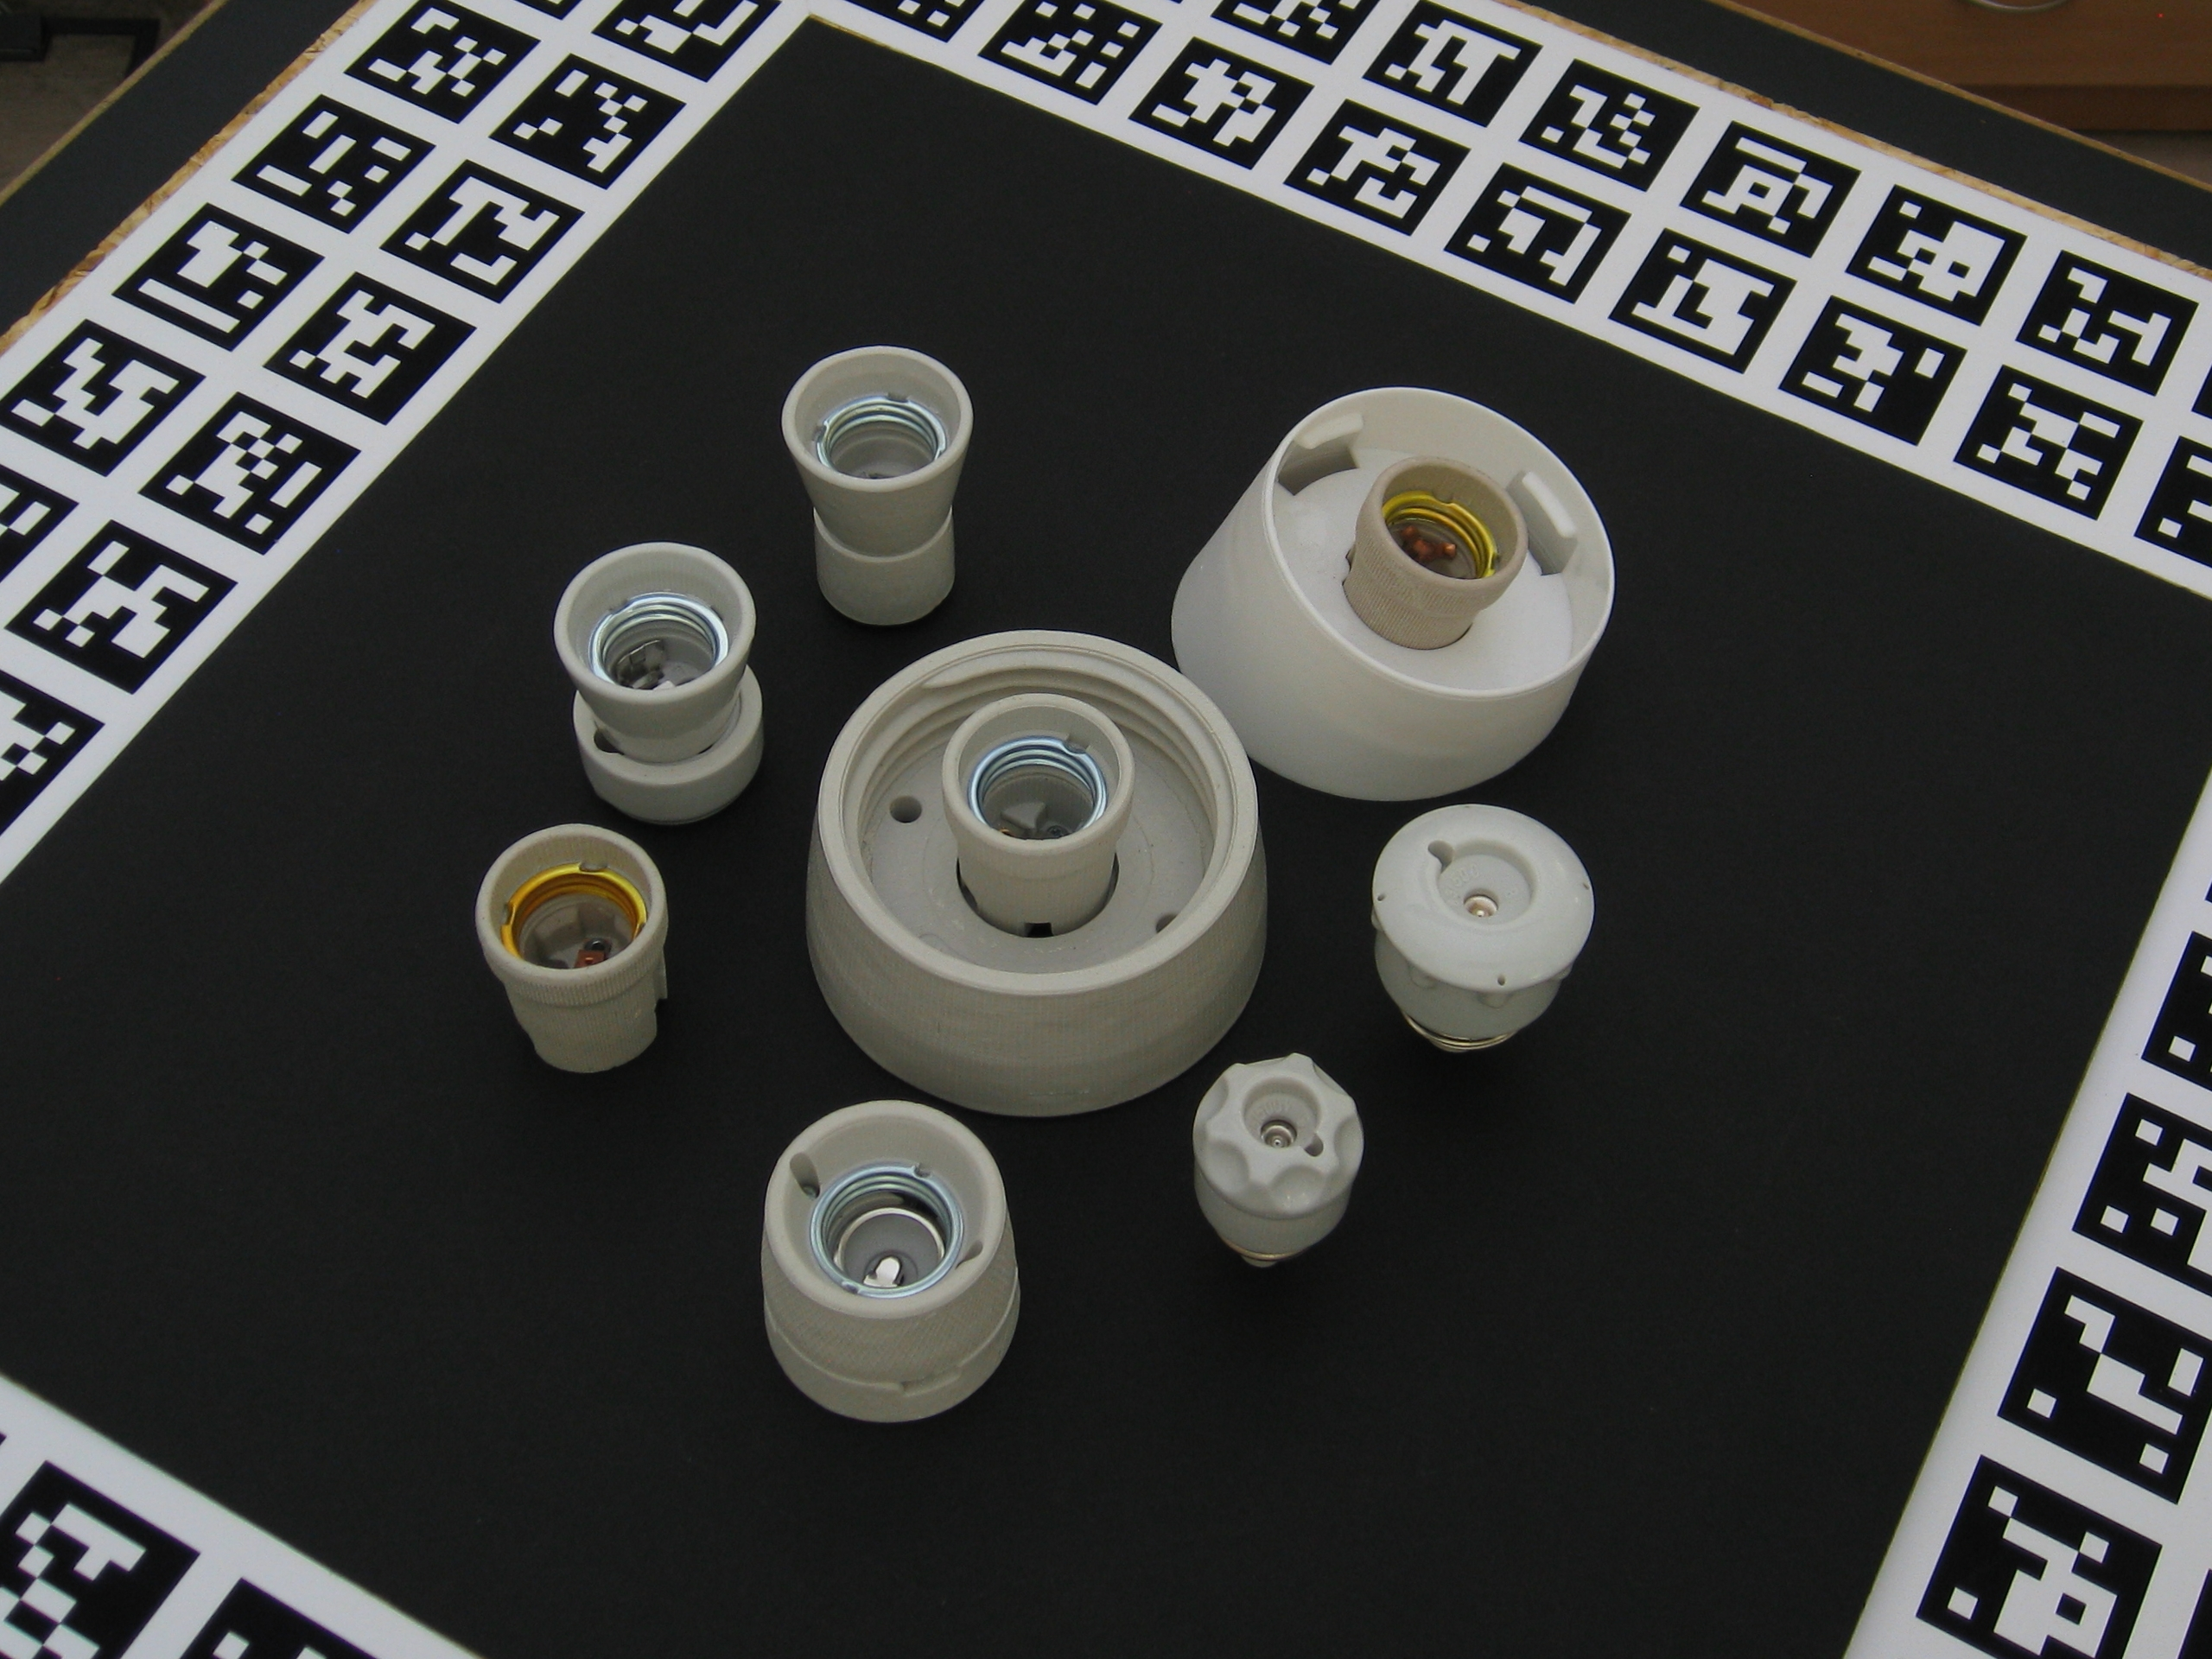
\includegraphics[width=0.7\linewidth]{tless_example_test}
    	\caption{An example frame from the test dataset of T-Less.}
    	\label{fig:tless_example_test}
	\end{subfigure}
	\caption{Example frames from the T-Less dataset \cite{tless}.}
	\label{fig:tless_examples}
\end{figure}

The initial intention to completely annotate the medical images provided at the beginning of the project turned out to be not feasible (see chapter \ref{chapter:manual_annotation}). Instead, we chose the T-Less dataset to conduct the experiments with. Its objects are mostly texture-less  and of rather small size making them similar to surgical tools. Next to many human pose estimation datasets, there exist some datasets of objects too, like \cite{next_view_dataset}, \cite{pracsys_dataset} and \cite{rigid_body_dataset}. But the objects of T-Less resemble surgical tools more than the objects of those datasets.

The T-Less dataset was released in 2017 by Hoda\v{n} et al. \cite{tless}. It contains the object models of 30 industry-relevant real world objects. Two versions exist: one mesh of the object that was manually reconstructed using CAD software and one that was produced from RGB-D images. The objects were captured using a Primsense CARMINE 1.09, a Microsoft Kinect v2 and a Canon IXUS 950 IS. We used the photos of the Canon camera due to their quality and we do not need depth information, which is also provided by the CARMINE sensor and the Kinect. There are 1296 images of each object in the training set of the dataset, sampled in 10 degree steps in elevation and 5 degree azimuth. 20 test scenes, consisting of 504 images each, exist as well. Those are photographs of cluttered scenes of different complexity, with sometimes more than 15 objects visible. All training and test images are annotated with the ground-truth poses of the visible objects. The authors also provided a tool set to render the objects at a given pose, etc. Fig. \ref{fig:tless_example_train} shows an example frame from the training set and fig. \ref{fig:tless_example_test} an example frame from the test set. The training images of the other objects look similar to the one shown. The dataset provides depth images, as well, but this is irrelevant to our setting.

\section{Data Preparation}

The \textit{T-Less} dataset does neither provide 3D object coordinates nor segmentation masks. This is the reason why we rendered both ourselves. The script is part of the network package. Because the 16-bit TIFF object coordinate ground-truth files used up too much disk space when in original size they were cropped to the relevant area by determining the smallest box around the segmentation pixels. The images and segmentation masks were cropped to the same area and the camera matrices adjusted accordingly. We used 16-bit TIFF files instead of 32-bit because we deemed the accuracy of 16-bit enough.

\section{Metric}

%TODO clarify using formulas

To be able to measure the accuracy of the different architectures and training techniques, we provide a metric to capture different aspects of the predictions. The error rate usually indicates the accuracy of the network. But in certain circumstances it makes sense to evaluate the predictions in a different way. One scenario that can occur is that the network predicts very inaccurate object coordinates at the border of the object's pixels. Since RANSAC eliminates outliers, the pose might not be much worse than a pose recovered from a prediction without outliers. The metric we defined measures the euclidean distance of the predicted and ground-truth coordinates, the number of inliers (pixels whose euclidean distance is below a certain threshold), as well as the angle error of the rotation and the euclidean distance of the translation of the recovered pose. This means, that the metric captures two error values based on the actual prediction and two based on the recovered pose. The script that we provide automatically calculates the mean but also outputs the median at 25, 50 and 75\% of the sorted error values. We assumed that the median at 50\% offers a good description of the accuracy of the network and used it to compare architectures and training setups.

\section{Training Experiments}

This section describes the configuration of the different training experiments. The chronological order of the experiments is reflected here. First, we compare the SGD and Adam optimizer in \ref{subsection:optimizers}. Then we evaluate the different architectures against each other in \ref{subsection:architectures}. Finally, asses the two training strategies training from scratch and incremental training in \ref{subsection:experiments_online_learning}. We conducted all experiments on the object model $01$ of the T-Less dataset. The image dimension was set to 500 pixels (for width and height), which is larger than the largest area covering an object in any image. All experiments were run using the training data of the object model $01$. For some experiments, we used only a subset of the available images (see Sections \ref{subsection:experiments_online_learning} and \ref{subsection:experiments_active_learning}) but we always split the data into 70\% training images and 30\% validation images. The axis labeled \textit{epochs} in loss graphs denotes the number of epochs the training was run for. Each epoch consisted of 1000 iterations in every experiment.

\begin{table}[]
\centering
\begin{tabular}{|l||lllll|}
\hline
Run                                                     & 1     & 2      & 3       & 4        & 5         \\ \hline \hline
\rowcolor{Gray}
Epochs                                                  & 30    & 45     & 55      & 65       & 70        \\
\begin{tabular}[c]{@{}l@{}}Learning\\ Rate\end{tabular} & 0.001 & 0.0001 & 0.00001 & 0.000001 & 0.0000001 \\  \hline
\end{tabular}
\caption{The configuration of the SGD optimizer used in the experiment to compare SGD and Adam.}\label{table:experiments_optimizers_sgd}
\end{table}

\subsection{Optimizers} \label{subsection:optimizers}  

\begin{figure}[!tbp]
	\centering
	\begin{subfigure}[t]{0.48\textwidth}
			\begin{tikzpicture}
  				\begin{axis}[cycle list name=tb, 
                 grid=both,
                 grid style={solid,gray!30!white},
                 axis lines=middle,
    			 xmin = 0,
    			 xmax = 100,
    			 ymin = 0,
    			 ymax = 3,
                 xlabel={epoch},
                 ylabel={loss},
                 x label style={at={(axis description cs:0.5,-0.1)},anchor=north},
                 y label style={at={(axis description cs:-0.1,.5)},rotate=90,anchor=south},]
      			\addplot[smooth,tb_color_1] table [x=Step, y=Value, col sep=comma] {experiments/model1/exp1_adam_l1/train_loss.csv};
      			\addplot[smooth,tb_color_2] table [x=Step, y=Value, col sep=comma] {experiments/model1/exp1_sgd/train_loss.csv};
      			\addlegendentry{Adam}
				\addlegendentry{SGD}
    			\end{axis}
			\end{tikzpicture}
		\caption{Training losses.}
	\end{subfigure}
	\hfill
	\begin{subfigure}[t]{0.48\textwidth}
			\begin{tikzpicture}
  				\begin{axis}[cycle list name=tb, 
                 grid=both,
                 grid style={solid,gray!30!white},
                 axis lines=middle,
    			 xmin = 0,
    			 xmax = 100,
    			 ymin = 0,
    			 ymax = 3,
                 xlabel={epoch},
                 ylabel={loss},
                 x label style={at={(axis description cs:0.5,-0.1)},anchor=north},
                 y label style={at={(axis description cs:-0.1,.5)},rotate=90,anchor=south},]
      			\addplot[smooth,tb_color_1] table [x=Step, y=Value, col sep=comma] {experiments/model1/exp1_adam_l1/val_loss.csv};
      			\addplot[smooth,tb_color_2] table [x=Step, y=Value, col sep=comma] {experiments/model1/exp1_sgd/val_loss.csv};
      			\addlegendentry{Adam}
				\addlegendentry{SGD}
    			\end{axis}
			\end{tikzpicture}
		\caption{Validation losses.}
	\end{subfigure}
	\caption{Training and validation losses of Adam and SGD used to train architecture 1. The plot is cropped on the $y$-axis to enhance the differences.}
	\label{fig:experiments_adam_sgd_loss}
\end{figure} 

To obtain the best optimizer for further experiments, we compared SGD and Adam using the first architecture we constructed. This architecture consists of 23 layers and has a receptive field-size of 99. The hyper-parameters $\beta_1$ and $\beta_2$ of the Adam optimizer were left at the default values set by Keras, which are $0.9$ and $0.999$, respectively. The more complex configuration of the SGD optimizer is given in Table \ref{table:experiments_optimizers_sgd}. Fig. \ref{fig:experiments_adam_sgd_loss} shows the loss of both experiments during training. The SGD optimizer profits from the reduction of the learning rate around step 30, visible as the small step in the training loss. This could imply that further tuning of the training parameters of SGD could lead to better results than the displayed ones. But since the Adam optimizer does not need manual fine-tuning of its hyper-parameters and performs visibly better than SGD, we chose Adam as the optimizer for all following experiments. We based our conclusion that Adam is the superior optimizer for our network solely on the loss values. Since we trained the same network architecture twice and only varied the optimizers, better error rates mean better overall results.

\subsection{Loss Functions}

\begin{table}[]
\centering
\begin{tabular}{|l||llll|}
\hline 
 Loss  & \begin{tabular}[c]{@{}l@{}}Object Coordinate\\ Error\end{tabular} & Inliers & Angle Error & Distance Error \\ \hline \hline \rowcolor{Gray}
L1 & 0.3413                                                            & 1738    & 0.0281      & 4.5574         \\
L2 & 0.8188                                                            & 1617    & 0.1090      & 8.3138 \\ \hline   
\end{tabular}
\caption{The metrics of the experiments comparing the loss functions.}
\label{table:experiments_loss_functions}
\end{table}

%TODO maybe rewrite this "to prove our statment...." -> did we prove it???

To prove our statement that the L1 loss is more suitable than the L2 loss for our application, we conducted another training run using the L2 loss and compared it to the run using the L1 loss of the previous experiment. The loss function comparisons are depicted in \ref{fig:experiments_l1_l2_loss} but are omitted here, due to their limited comparability. To obtain the L2 loss, we removed taking the square root in computing the loss which naturally results in higher error rates. Table \ref{experiments_loss_functions} shows the metrics of the experiments with the different loss functions. The L1 loss offers clearly superior accuracy and is used in all further experiments.

\subsection{Architectures} \label{subsection:architectures}

%TODO table of training parameters -> different batch sizes etc

\begin{figure}[!tbp]
	\centering
	\begin{subfigure}[t]{0.48\textwidth}
			\begin{tikzpicture}
  				\begin{axis}[cycle list name=tb, 
                 grid=both,
                 grid style={solid,gray!30!white},
                 axis lines=middle,
                 xlabel={epoch},
                 ylabel={loss},
                 x label style={at={(axis description cs:0.5,-0.1)},anchor=north},
                 y label style={at={(axis description cs:-0.1,.5)},rotate=90,anchor=south},]
      			\addplot[smooth,tb_color_1] table [x=Step, y=Value, col sep=comma] {experiments/model1/exp1_adam_l1/train_loss.csv};
      			\addplot[smooth,tb_color_3] table [x=Step, y=Value, col sep=comma] {experiments/model3/exp1/train_loss.csv};
      			\addplot[smooth,tb_color_6] table [x=Step, y=Value, col sep=comma] {experiments/model6/exp1/train_loss.csv};
      			\addlegendentry{Architecture 1}
				\addlegendentry{Architecture 3}
				\addlegendentry{Architecture 6}
    			\end{axis}
			\end{tikzpicture}
		\caption{Training losses.}
	\end{subfigure}
	\hfill
	\begin{subfigure}[t]{0.48\textwidth}
			\begin{tikzpicture}
  				\begin{axis}[cycle list name=tb, 
                 grid=both,
                 grid style={solid,gray!30!white},
                 axis lines=middle,
                 xlabel={epoch},
                 ylabel={loss},
                 x label style={at={(axis description cs:0.5,-0.1)},anchor=north},
                 y label style={at={(axis description cs:-0.1,.5)},rotate=90,anchor=south},]
      			\addplot[smooth,tb_color_1] table [x=Step, y=Value, col sep=comma] {experiments/model1/exp1_adam_l1/val_loss.csv};
      			\addplot[smooth,tb_color_3] table [x=Step, y=Value, col sep=comma] {experiments/model3/exp1/val_loss.csv};
      			\addplot[smooth,tb_color_6] table [x=Step, y=Value, col sep=comma] {experiments/model6/exp1/val_loss.csv};
      			\addlegendentry{Architecture 1}
				\addlegendentry{Architecture 3}
				\addlegendentry{Architecture 6}
    			\end{axis}
			\end{tikzpicture}
		\caption{Validation losses.}
	\end{subfigure}
	\caption{Training and validation losses of the different architectures.}
	\label{fig:experiments_architectures_loss}
\end{figure} 

The experiments run on the different architectures were all performed using the Adam optimizer with the parameters mentioned in Section \ref{subsection:optimizers} and the L1 loss. The major difference between the experiments is the architecture itself. The training process were run for a different number of iterations because some architectures converged earlier than others. The different losses are displayed in fig. \ref{fig:experiments_architectures_loss}.

\subsection{Online Learning} \label{subsection:experiments_online_learning}

%TODO  Check if number of images in plot is correct
      			
\begin{figure}[!tbp]
	\centering
	\begin{subfigure}[t]{0.48\textwidth}
			\begin{tikzpicture}
  				\begin{axis}[cycle list name=tb, 
                 grid=both,
                 grid style={solid,gray!30!white},
                 axis lines=middle,
                 xlabel={epoch},
                 ylabel={loss},
                 x label style={at={(axis description cs:0.5,-0.1)},anchor=north},
                 y label style={at={(axis description cs:-0.1,.5)},rotate=90,anchor=south},]
      			\addplot[smooth,tb_color_1] table [x=Step, y=Value, col sep=comma] {experiments/model1/exp1_adam_l1/train_loss.csv};
      			\addplot[smooth,tb_color_2] table [x=Step, y=Value, col sep=comma] {experiments/model1/exp2/train_loss.csv};
      			\addplot[smooth,tb_color_3] table [x=Step, y=Value, col sep=comma] {experiments/model1/exp3/train_loss.csv};
      			\addplot[smooth,tb_color_4] table [x=Step, y=Value, col sep=comma] {experiments/model1/exp4/train_loss.csv};
      			\addplot[smooth,tb_color_5] table [x=Step, y=Value, col sep=comma] {experiments/model1/exp5/train_loss.csv};
      			\addplot[smooth,tb_color_6] table [x=Step, y=Value, col sep=comma] {experiments/model1/exp6/train_loss.csv};
      			\addlegendentry{All}
      			\addlegendentry{500}
				\addlegendentry{250}
				\addlegendentry{100}
				\addlegendentry{50}
				\addlegendentry{25}
    			\end{axis}
			\end{tikzpicture}
		\caption{Training losses.}
	\end{subfigure}
	\hfill
	\begin{subfigure}[t]{0.48\textwidth}
			\begin{tikzpicture}
  				\begin{axis}[cycle list name=tb, 
                 grid=both,
                 grid style={solid,gray!30!white},
                 axis lines=middle,
                 xlabel={epoch},
                 ylabel={loss},
                 x label style={at={(axis description cs:0.5,-0.1)},anchor=north},
                 y label style={at={(axis description cs:-0.1,.5)},rotate=90,anchor=south},]
      			\addplot[smooth,tb_color_1] table [x=Step, y=Value, col sep=comma] {experiments/model1/exp1_adam_l1/val_loss.csv};
      			\addplot[smooth,tb_color_2] table [x=Step, y=Value, col sep=comma] {experiments/model1/exp2/val_loss.csv};
      			\addplot[smooth,tb_color_3] table [x=Step, y=Value, col sep=comma] {experiments/model1/exp3/val_loss.csv};
      			\addplot[smooth,tb_color_4] table [x=Step, y=Value, col sep=comma] {experiments/model1/exp4/val_loss.csv};
      			\addplot[smooth,tb_color_5] table [x=Step, y=Value, col sep=comma] {experiments/model1/exp5/val_loss.csv};
      			\addplot[smooth,tb_color_6] table [x=Step, y=Value, col sep=comma] {experiments/model1/exp6/val_loss.csv};
      			\addlegendentry{All}
      			\addlegendentry{500}
				\addlegendentry{250}
				\addlegendentry{100}
				\addlegendentry{50}
				\addlegendentry{25}
    			\end{axis}
			\end{tikzpicture}
		\caption{Validation losses.}
	\end{subfigure}
	\caption{Training and validation losses of the experiments of training architecture \textbf{1} from scratch but not with all images. The keys are the number of images used in training.}
	\label{fig:experiments_online_sratch_loss}
\end{figure} 

% Nochmal zusammenfassen scratch vs inkrementell

\subsection{Active Learning} \label{subsection:experiments_active_learning}

% Training on one side only -> provide metric results -> training on bad images -> new metrics

\subsection{Runtime Analysis}

This section analyses the inference runtimes of the different architectures. Deeper networks need longer to perform training and an inference run on an image, which is reflected by table ...

\subsection{Limitations}

% No challenge yet, difficult to tell how good network is -> no baseline!

% T-Less dataset contains only unoccluded images

% This way of comparing training procedures is owned to the timeframe of this work -> maybe L2 works better for model 5, etc., we generalize from one model to all others

% Create metric for images that the network produces bad predictions for, e.g. reprojection error for contradicting object coordinates, difference between segmentation mask rendered using the predicted pose and the ground-truth segmentation mask -> was not possible because we couldn't annotate images of the Endovis dataset

% Maybe training - validation ratio should be more like 90 - 10

% Difficult to say how the network would perform on the Endovis dataset -> we don't know if the networks with larger receptive field-size predict based on the letters
\chapter{Discussion}\label{chapter:discussion}

Before discussing the outcomes of this work, we want to state a general remark. Our goal of training the network on the Endoscopic Vision Challenge dataset was not achievable, as we were not provided with the correct 3D object models. It is difficult to tell, how the networks would have performed on this dataset, as it appears to be more challenging in terms of image quality, occlusion, etc.

\section{Manual Annotation Process} \label{section:discussion_manual_annotation_process}

\begin{table}
\centering
    \begin{tabular}{|c||ccccc|} \hline
\diagbox{\# Object}{Image} & 0000.jpg & 0150.jpg & 0250.jpg & 0350.jpg & 0500.jpg \\ \hline\hline
\rowcolor{Gray}
01           &  0:53 & 2:29 & 0:20 & 0:03 & 0:06 \\ \hline
\end{tabular}
	\caption{The table shows the \textbf{absolute difference} between in minutes between correcting a pose using the controls of \ac{6dpat} and the new rotation feature. The comparison was only performed exemplary for object model 01 due to the limited time-frame of this work.} 
	\label{table:6dpat_improved_times}
\end{table}

The process of manually recovering poses using \ac{6dpat} comes along with some peculiarities, which we discuss here. By creating some annotations ourselves, we figured out that one of the bottlenecks of the program is the correction of poses after the initial position and rotation has been recovered from the clicked correspondences. The reason is that adjusting the values of the rotation and position by hand using the provided controls is slow and a try-and-error process. By trying to enter a higher rotational degree, the correct value was often surpassed. 

Despite the limited time of this work, we decided finally to improve the correction procedure by implementing functionality that allows easy rotation of the object model of a pose using the mouse. To make use of this new feature, the user has to select a pose to edit from the drop down list of poses and rotate the object model that is displayed by the pose editor (not pose viewer). This concept allowed the author to achieve the difference in times presented in Table \ref{table:6dpat_improved_times}. The discrepancy was computed only for the time needed to correct a pose, i.e. the time needed for clicking correspondences was not considered. This is not an empirical study and the superiority of the rotation method compared to manually editing the numbers needs to be proven for many images and datasets. But the provided times can serve as an indicator that directly rotating the object can be faster.

Next to \ac{6dpat}, we also faced some issues regarding the datasets themselves. Initially, a desired feature was to present another unannotated image after the user finishes annotating all poses in the current image. This is not feasible for multiple reasons. First of all, a user might still not be content with the poses. Selecting the next image programmatically could happen too early and thereby disrupt the annotation process of the user. The datasets can also have very distinct characteristics, which require the user to choose the next image manually. For a dataset like T-Less, many images have to be skipped due to their similarity. A network trained on one view on an object only, will likely predict inaccurate poses for a different view showing other characteristics of that object. The dataset of the Endoscopic Vision Challenge has less similar consecutive images.

The diversity of available datasets (see Section \ref{section:experiments_datasets} for a selection of datasets) is also the reason why the program does not provide functionality to initialize the next poses based on the ones in the last image. This feature would imply too many assumptions on the dataset and, in the worst case, cause more work for the user. 

While trying to annotate the images of the Endoscopic Vision Challenge dataset, it became clear that proper 3D models are crucial for successful annotation. To temporarily annotate the medical images, 3D surgical tools were downloaded from the internet as a replacement for the missing object models. But having a different shape and also missing the distinctive features of the real objects makes it very difficult to estimate the ground-truth pose. The influence of contradicting annotated poses during training of a network is not clear. The author of this work strongly recommends to obtain the correct 3D models before annotating the Endoscopic Vision Challenge images. The issue of the object models not fitting the segmentation mask can be seen in \fig \ref{fig:6dpat_sfb_segmentation}. \fig \ref{fig:6dpat_sfb_image} shows the actual image and the discrepancy between the object models and image pixels.

\begin{figure}
	\begin{subfigure}[t]{0.47\textwidth}
		\centering
    	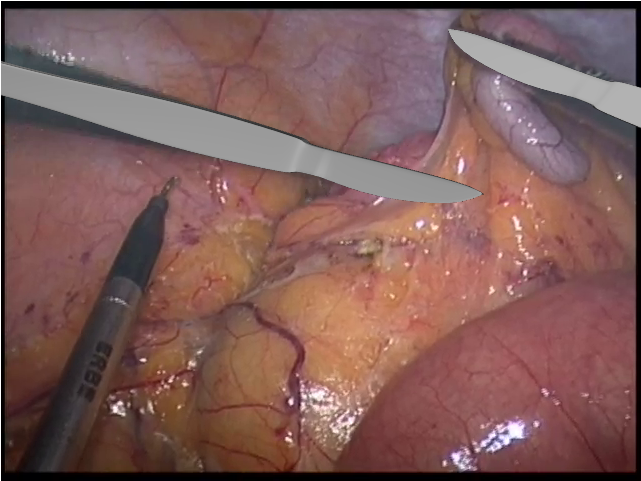
\includegraphics[width=\linewidth]{6dpat_sfb_image}
    	\caption{An image from the medical images dataset annotated using \ac{6dpat}. The correct rotation and translation are difficult to estimate without the correct 3D models.}
    	\label{fig:6dpat_sfb_image}
	\end{subfigure} 
	\hfill
	\begin{subfigure}[t]{0.47\textwidth}
		\centering
    	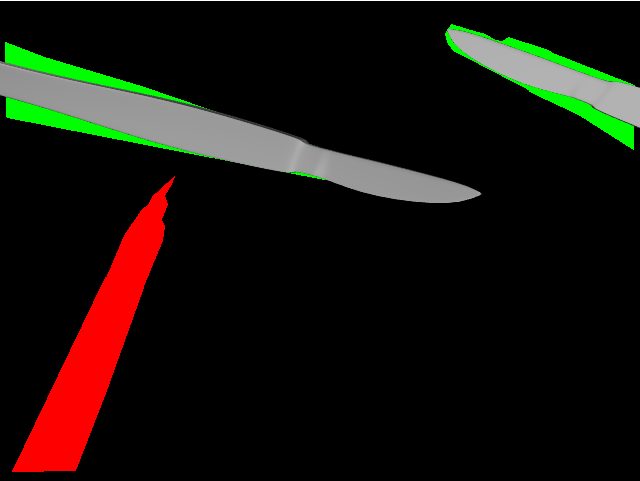
\includegraphics[width=\linewidth]{6dpat_sfb_segmentation}
    	\caption{The corresponding segmentation image. The discrepancy between the segmentation masks and the object model is the clearly visible green area.}
    	\label{fig:6dpat_sfb_segmentation}
	\end{subfigure} 
	\caption{Example annotations of images of the Endoscopic Vision Challenge dataset. The object model is taken from \cite{3d_scalpel_online}.}
	\label{fig:6dpat_sfb}
\end{figure} 

A general problem of any dataset can be seen in Appendix \ref{appendix:example_annotations} in form of the rotational error of manually annotated images. If the offset is similar in all recovered poses, this might not cause any trouble. If not, a network might be trained with contradicting object coordinates. There is no simple solution to this problem. Distinct characteristics of the object models could reduce this effect significantly, like the letters on the surgical tools in the Endoscopic Vision Challenge dataset or the notch of object model 01 of the T-Less dataset.

We think that \ac{6dpat} already resembles a program that can be used to annotate pose estimation datasets, efficiently and effectively already. Nevertheless, we provide improvement suggestions in Chapter \ref{chapter:future_work}.

\section{Semi-Automatic Annotation Process}

This section discusses the results of the experiments that we conducted using the network architectures of Chapter \ref{chapter:semi_automatic}. To this end, we analyze the outcomes in the order they appeared in Chapter \ref{chapter:experiments}. First, we want to make clear that some of the ways how we inferred conclusions underly some restrictions and are owed to the limited time of this work. An incremental training approach might have worked better for architectures 2 and 3, for example. We do not see this as a significant issue but it has to be kept in mind when using the results for further research.

The comparison of the different architectures of the neural network show that batch normalization offer superior accuracy without further fine-tuning. We provide our interpretation of the differences between the other designs here. We conclude that the reduction of the receptive field-size without increasing the network's depth leads to a higher training and validation error. 

This can be seen in the discrepancy between the loss curves of architecture 1 and 3, since architecture 3 is as deep as architecture 1 (both 23 layers) but with a reduced receptive field-size. Architecture 2 compensates the increased error related to the field-size by deeper design (35 layers). Architecture 5 achieves an error as low as architecture 1. Although its receptive field-size is smaller than that of architecture 2 (59 opposed to 67), we increased the number of layers to 50. Intuitively, by seeing less data (smaller receptive field-size) the network has to compensate this by being able to store more information somehow, thus the need for more layers.

One reason why architecture 5 achieves better meric results on the test set of the T-Less dataset than architecture 1 could be that the objects in the test scenes often occlude each other. Due to architecture 1's larger receptive field-size it could be that the network predicts coordinates based on distinctive characteristics of the objects which are not visible in some cases. 

It also looks like all architectures memorize the training data quite well and achieve high pose inlier rates. But this does not hold for the metrics on the test set, although the test scenes are similar in terms of lightning conditions and image quality. We are unsure how the large drop of the performance of the networks on the test scene images compared to the training images came to exist.

Rad \etal report an average pose inlier rate of all objects visible in the test scene of 53.5 in \cite{bb8}. To the best of our knowledge, this is the only work providing an inlier rate on the T-Less dataset without using depth. This number is significantly higher than the accuracy we achieved. We expected even better results from our networks because the location of the object is already defined by the segmentation mask. 

Our initial assumption was that the networks are too deep and overfitted towards the data they were trained on. Despite the similar lightning conditions of the test images, we thought that the networks had taken in too many details of the training images. Since the validation images were taken from the pool of available training images, overfitting to the conditions of the training images can not be entirely prevented by such a validation set. But architecture 5 achieves the best pose inlier rate on the test set. Thus, it might be that the architectures are actually too shallow. Unfortunately, we were not able to explore this in depth in favor of examining the different training strategies.

The overall appearance of the validation losses of the incremental approaches is difficult to interpret. The network seems to overfit but even if the training runs had been stopped in the valleys visible in \fig \ref{fig:experiments_online_sratch_90_10_validation_loss_arch1}, there would be a large gap compared to the training from scratch, still.

We cannot give a final statement why the incremental approach results in such an inferior validation loss. We assume that there is a way to improve this method so that it reaches the same level like the training from scratch. A reason for the inconsistent loss could be the trainable batch normalization. Training the network with 50 images first and then fixing the batch normalization weights could help decrease the validation loss when further training the network with datasets of 25 images. Although we expelled the SGD optimizer at the beginning of the experiments it could be that it is able to provide better results than Adam. We conclude this from the loss graphs of the incremental experiments, as the spiky curves could mean that Adam is not able to properly compute the learning rate. A very small rate set for SGD could yield different results. But for now, we have to recommend to train the network from scratch every time the user has manually annotated another batch of images.

The active training scheme on the other hand did provide better validation losses, i.e. selecting the images with the smallest IoU with the ground-truth segmentation masks reduced the validation loss significantly. This way, the validation loss of the experiment of training the network with 100 images from scratch was reached. Training with 50 of these images first and then incrementally training the network with the remaining 50 images resulted in a high validation loss. The results on the test set imply that this does not reliably mean that the network performs better in general. This is a sever issue and needs further investigation before drawing any conclusions.

We still suggest using a network together with \ac{6dpat}. We think that an unannotated dataset like \ac{evc} can still profit from the approximate locations predicted by a neural network. Despite the implication by the provided metric results that most poses are very inaccurate, visually checking the inferred poses of the test scene indicates that only small rotational corrections are necessary, which can be achieved quickly with the rotation feature of \ac{6dpat}.
\chapter{Future Works} \label{chapter:future_work}

To provide an outlook how the manual annotation process can be improved in the future, we provide some suggestions here. An important feature that should be implemented in \ac{6dpat} is allowing to move the object models around on the displayed image by dragging and them using the mouse. The initial poses using the clicking procedure are already sufficiently accurate in many cases. But when the camera is looking along an axis of the object, the position can be far off. The user can correct these poses with the provided controls. But the implemented rotation feature indicates that editing a pose by mouse can be faster which probably also holds for the position of an object.

The binding of the neural network to the program does not allow to load the weights of the net and persist this state in the memory of the computer. In case that the user wants to annotate a large dataset of just one object, they could profit from a feature allowing to keep the weights in memory instead of loading them each time the inference process is started. This way, predicting the pose for only one image could be achieved in significantly less time. Running the network to predict the pose of one object in a large amount of images amortizes the loading of the weights.

Another suggested step is to fully incorporate the network in the annotation tool. This way, inexperienced users can profit from the network without the need for an expert to run the network inference. There is probably no way to automatize the setup process, as this requires knowledge neural networks. In an ideal setting, this interference can be reduced to a minimum and users are introduced to the most relevant parameters only, which they can set from within the program.

Because the neural network is trained for one object only, the time-intensive step (proportional to the overall time needed for inference on one image) of loading the trained weights has to be performed before predicting poses for different objects. The frame of this work was to explore neural networks trained for one object only, it is therefore not known whether this overhead of loading the weights can be reduced.

% maybe train network on test images and try on training images

% dropout nicht weiter erforscht, koennte aber gut sein, dass das overfitten verhinderbar ist, dann koennte es auch gute ergebnisse liefern, vor allem fuer das inkrementelle training

% batchnorm von trainiertem netz nehmen, batch norm auf nicht lernbar setzen und das dann fuer das inkrementelle training benutzen
\begin{appendices}

\chapter{Example Manual Annotations} \label{appendix:example_annotations}

\begin{figure}[!tbp]
	\centering
	\vspace{5mm}
	\begin{subfigure}[t]{0.47\textwidth}
		\centering
    	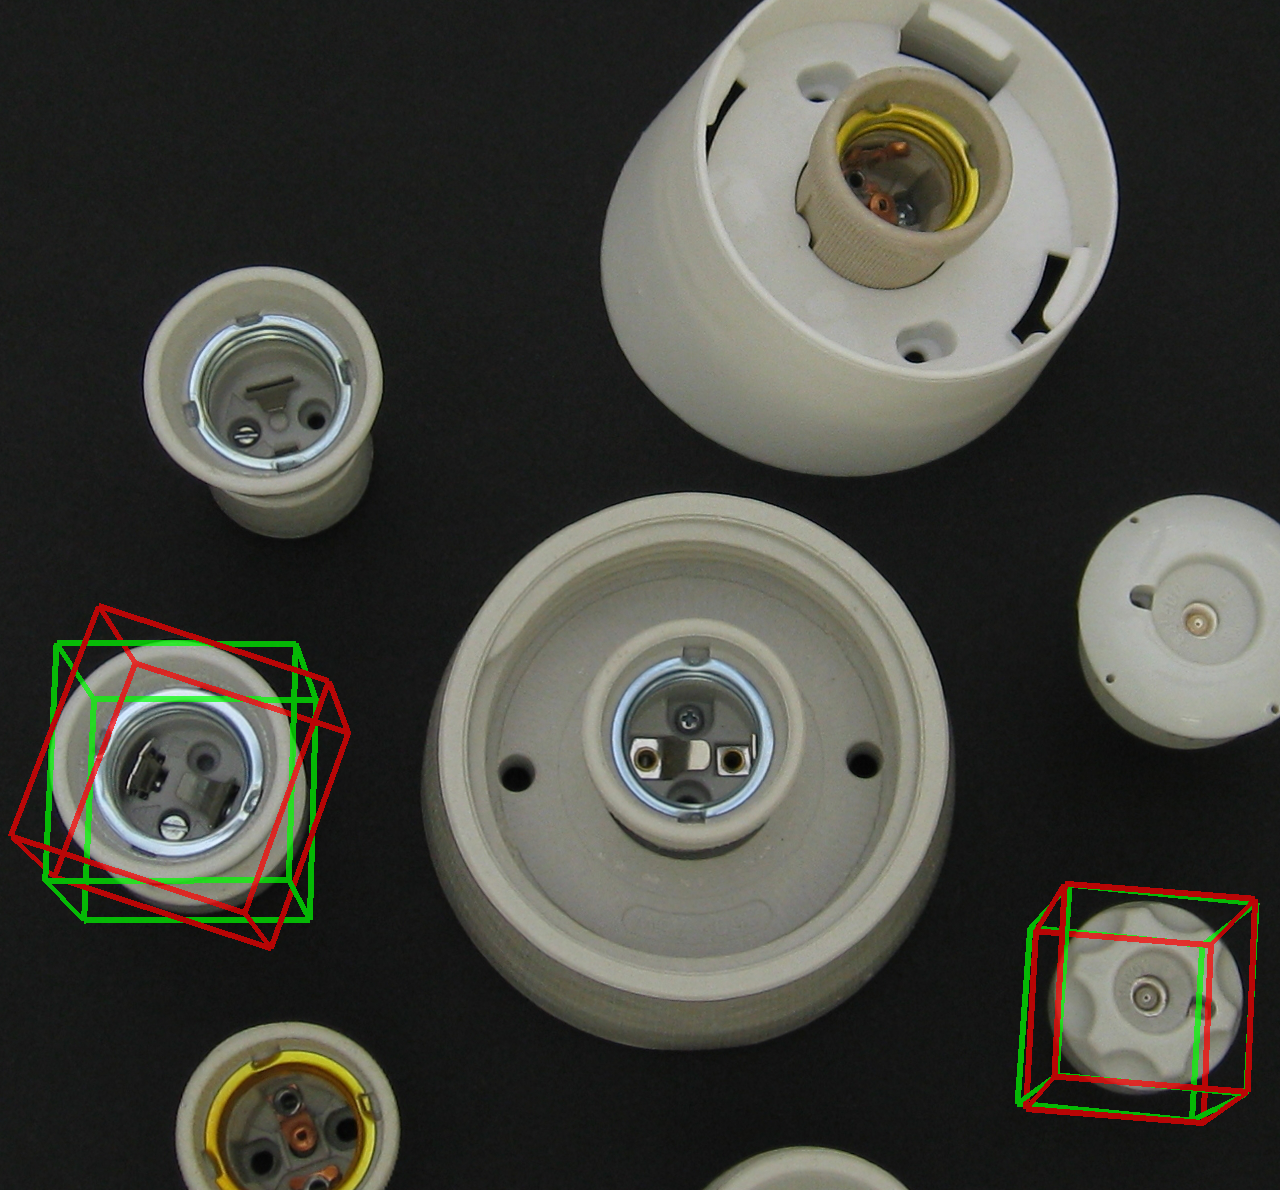
\includegraphics[width=\linewidth]{6dpat_exp_0000}
    	\caption{Image 0000.jpg.}
	\end{subfigure}
	\hfill
	\begin{subfigure}[t]{0.47\textwidth}
		\centering
    	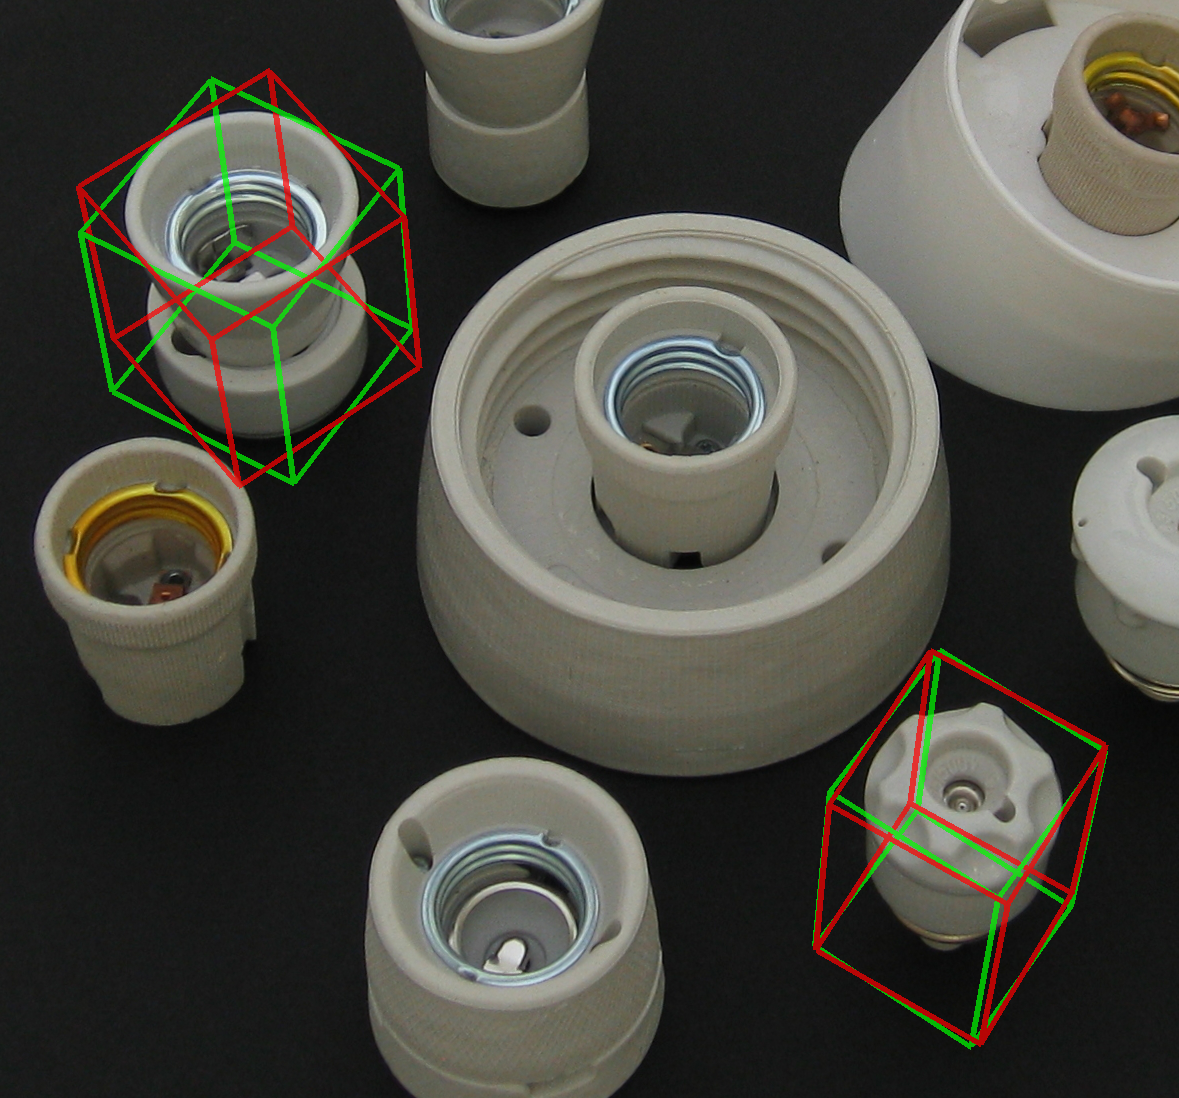
\includegraphics[width=\linewidth]{6dpat_exp_0150}
    	\caption{Image 0150.jpg.}
	\end{subfigure}
	\par\bigskip
	\begin{subfigure}[t]{0.47\textwidth}
		\centering
    	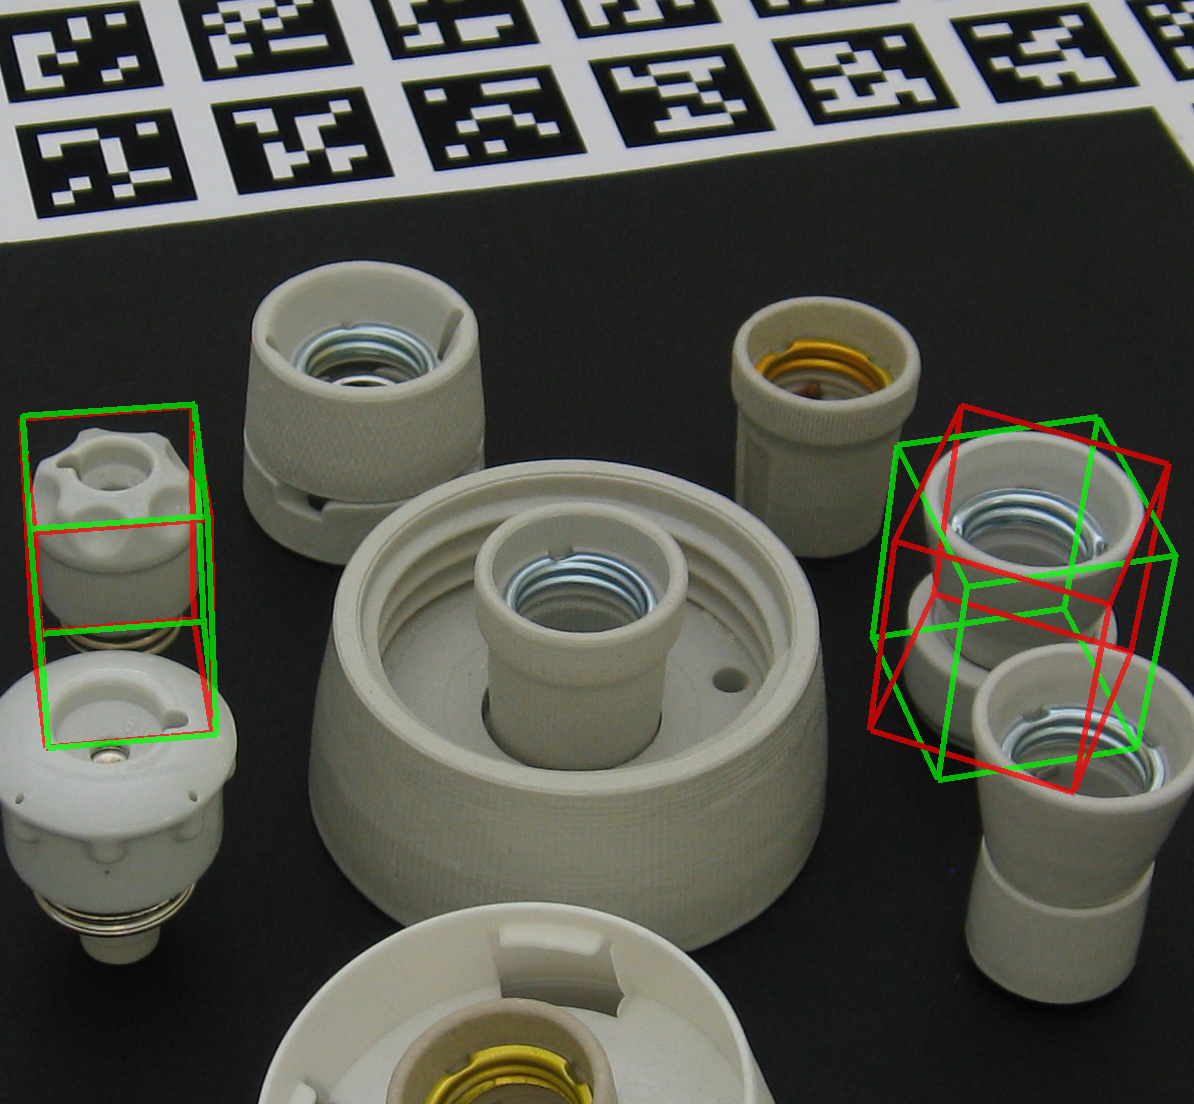
\includegraphics[width=\linewidth]{6dpat_exp_0250}
    	\caption{Image 0250.jpg.}
	\end{subfigure}
	\hfill
	\begin{subfigure}[t]{0.47\textwidth}
		\centering
    	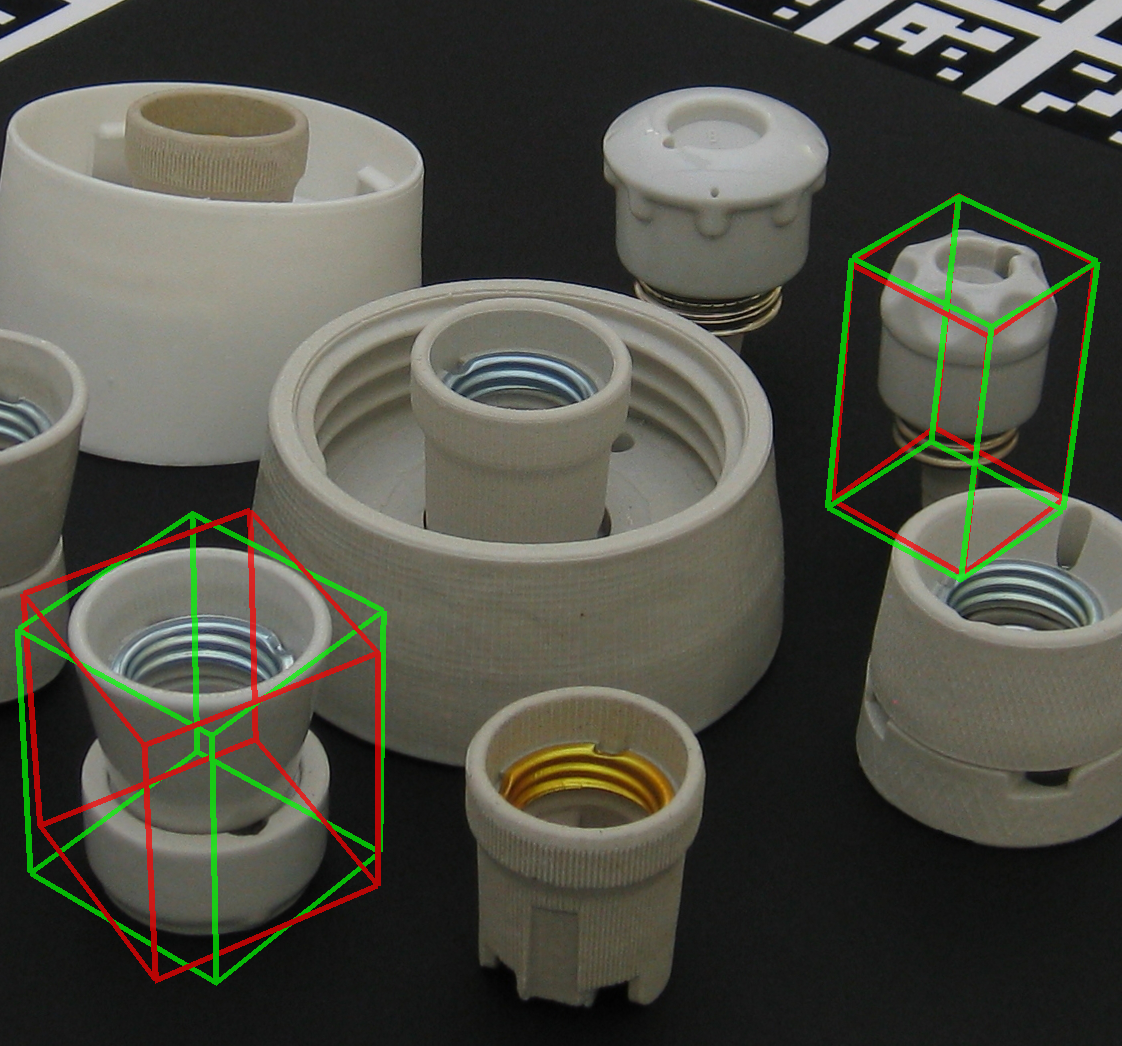
\includegraphics[width=\linewidth]{6dpat_exp_0350}
    	\caption{Image 0350.jpg.}
	\end{subfigure}
	\par\bigskip
	\begin{subfigure}[t]{0.47\textwidth}
		\centering
    	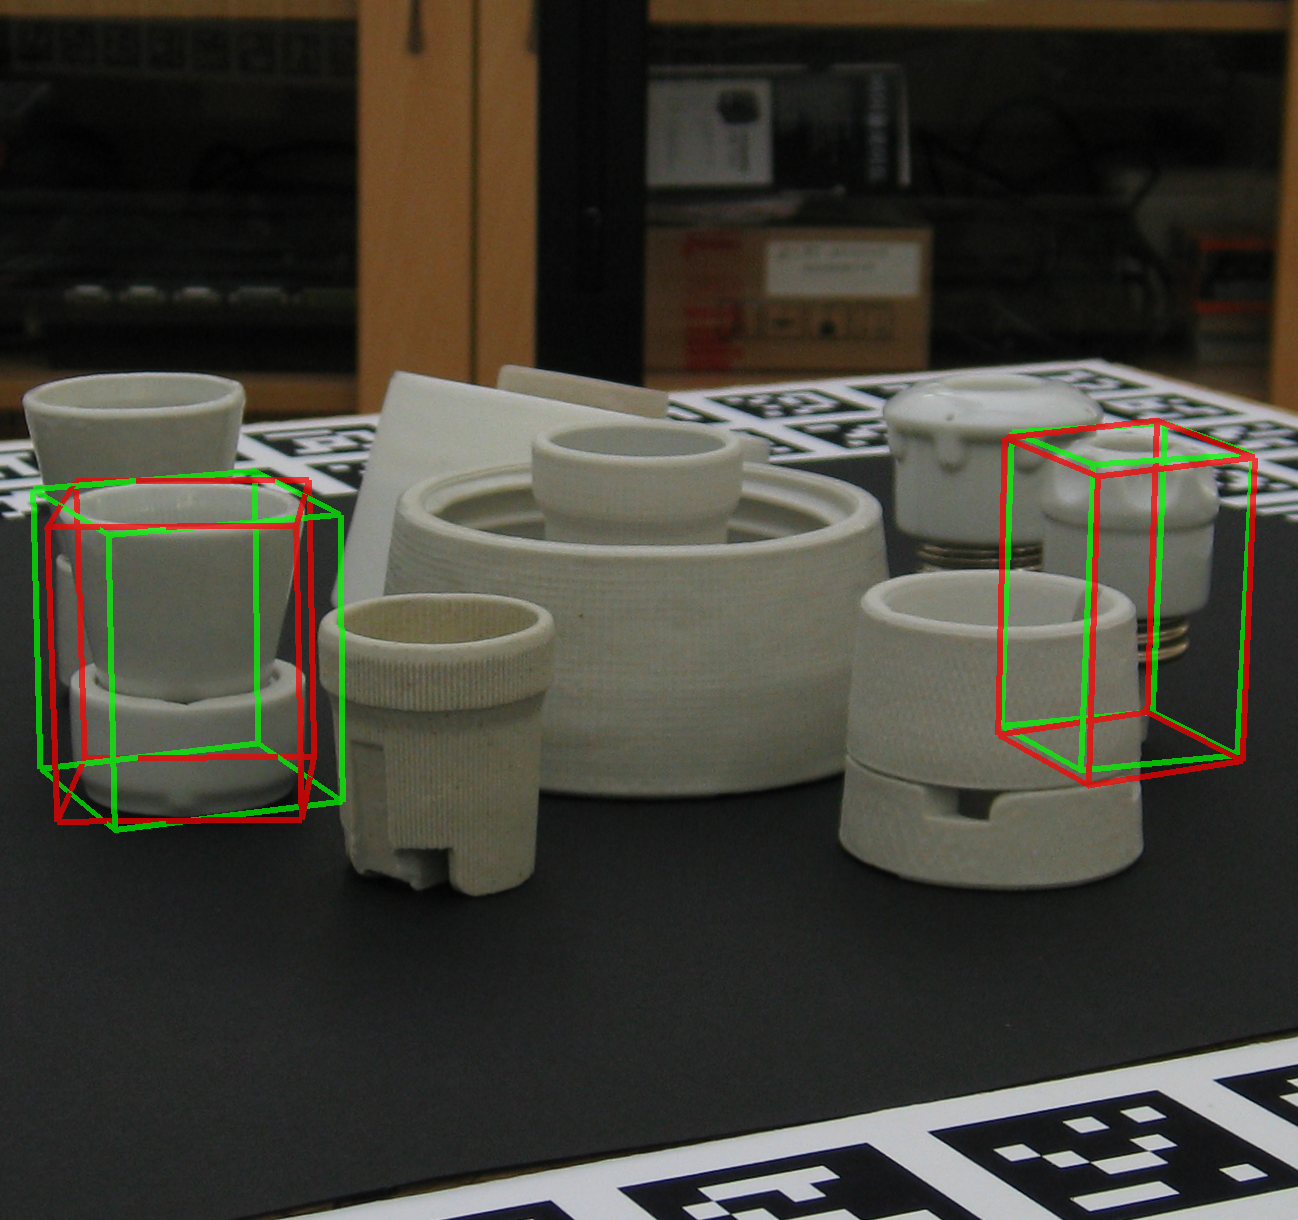
\includegraphics[width=\linewidth]{6dpat_exp_0500}
    	\caption{Image 0500.jpg.}
	\end{subfigure}
	\caption{Example images from test scene 7 of the T-Less dataset with the poses recovered using \ac{6dpat}. The images are cropped to the relevant area.}
\end{figure} 

\chapter{Network Architectures} \label{appendix:network_architectures}

\begin{figure}[!tbp]
	\centering
    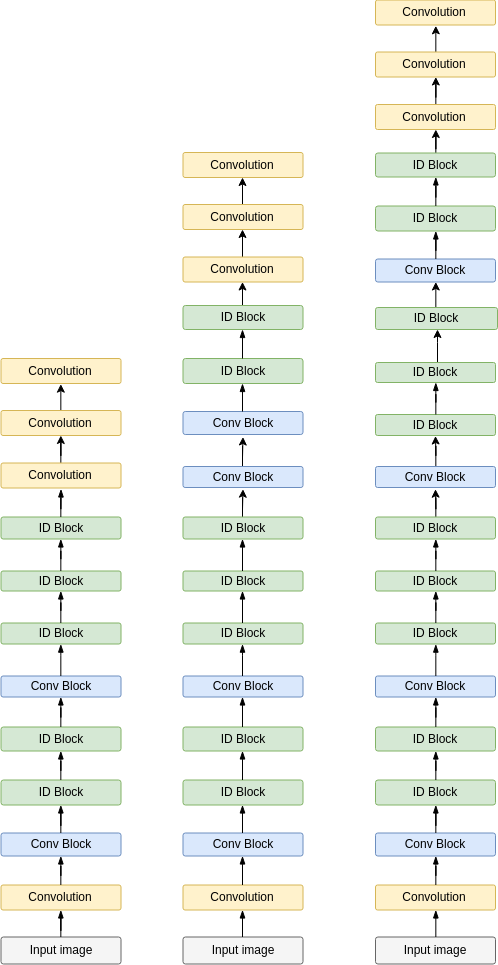
\includegraphics[width=0.7\linewidth]{network_architecture_comparison}
    \caption{The different architectures used in this work. Architectures 1 and 3 use the leftmost structure with a total of 23 convolutional layers. We constructed architecture 2 using the layout in the middle with 35 layers. Architectures 4, 5 and 6 use the 50 layers structured as shown on the right, although architectures 4 and 6 employ dropout layers with different frequencies after each block and omit the batchnormalization layers. We omitted the batchnormalization layers in the other to structures for displaying purposes.}
    \label{fig:network_architecture_comparison}
\end{figure} 

\chapter{Experiments}

\begin{figure}[!tbp]
	\begin{subfigure}[t]{0.4\textwidth}
			\begin{tikzpicture}[scale=0.95]
  				\begin{axis}[cycle list name=tb, 
                 grid=both,
                 grid style={solid,gray!30!white},
                 axis lines=middle,
    			 xmin = 0,
    			 xmax = 50,
    			 ymin = 0,
    			 ymax = 15,
                 xlabel={step},
                 ylabel={value},
                 x label style={at={(axis description cs:0.5,-0.1)},anchor=north},
                 y label style={at={(axis description cs:-0.1,.5)},rotate=90,anchor=south},]
      			\addplot[smooth,tb_color_1] table [x=Step, y=Value, col sep=comma] {experiments/model1/exp1_adam_l1/train_loss.csv};
      			\addplot[smooth,tb_color_2] table [x=Step, y=Value, col sep=comma] {experiments/model1/exp1_adam_l2/train_loss.csv};
      			\addlegendentry{L1}
				\addlegendentry{L2}
    			\end{axis}
			\end{tikzpicture}
		\caption{Training losses.}
	\end{subfigure}
	\hspace{15mm}
	\begin{subfigure}[t]{0.4\textwidth}
			\begin{tikzpicture}[scale=0.95]
  				\begin{axis}[cycle list name=tb, 
                 grid=both,
                 grid style={solid,gray!30!white},
                 axis lines=middle,
    			 xmin = 0,
    			 xmax = 50,
    			 ymin = 0,
    			 ymax = 15,
                 xlabel={step},
                 ylabel={value},
                 x label style={at={(axis description cs:0.5,-0.1)},anchor=north},
                 y label style={at={(axis description cs:-0.1,.5)},rotate=90,anchor=south},]
      			\addplot[smooth,tb_color_1] table [x=Step, y=Value, col sep=comma] {experiments/model1/exp1_adam_l1/val_loss.csv};
      			\addplot[smooth,tb_color_2] table [x=Step, y=Value, col sep=comma] {experiments/model1/exp1_adam_l2/val_loss.csv};
      			\addlegendentry{L1}
				\addlegendentry{L2}
    			\end{axis}
			\end{tikzpicture}
		\caption{Validation losses.}
	\end{subfigure}
	\caption{Training and validation losses of the L1 and L2 loss of training architecture 1. The plot is cropped on the $y$-axis to enhance the differences.}
	\label{fig:experiments_l1_l2_loss}
\end{figure} 

\begin{figure}[!tbp]
	\centering
	\vspace{5mm}
	\begin{subfigure}[t]{0.47\textwidth}
		\centering
    	\includegraphics[width=\linewidth]{experiments/model2/0045_bounding_boxes}
    	\caption{Image 0045.jpg, pose recovered using architecture 2.}
	\end{subfigure}
	\hfill
	\begin{subfigure}[t]{0.47\textwidth}
		\centering
    	\includegraphics[width=\linewidth]{experiments/model2/0438_bounding_boxes}
    	\caption{Image 0438.jpg, pose recovered using architecture 2.}
	\end{subfigure}
	\par\bigskip
	\begin{subfigure}[t]{0.47\textwidth}
		\centering
    	\includegraphics[width=\linewidth]{experiments/model3/0045_bounding_boxes}
    	\caption{Image 0045.jpg, pose recovered using architecture 3.}
	\end{subfigure}
	\hfill
	\begin{subfigure}[t]{0.47\textwidth}
		\centering
    	\includegraphics[width=\linewidth]{experiments/model3/0438_bounding_boxes}
    	\caption{Image 0438.jpg, pose recovered using architecture 3.}
	\end{subfigure}
	\par\bigskip
	\begin{subfigure}[t]{0.47\textwidth}
		\centering
    	\includegraphics[width=\linewidth]{experiments/model5/0045_bounding_boxes}
    	\caption{Image 0045.jpg, pose recovered using architecture 5.}
	\end{subfigure}
	\hfill
	\begin{subfigure}[t]{0.47\textwidth}
		\centering
    	\includegraphics[width=\linewidth]{experiments/model5/0438_bounding_boxes}
    	\caption{Image 0438.jpg, pose recovered using architecture 5.}
	\end{subfigure}
	\caption{Example images from test scene 7 with rendered poses recovered by the architecture mentioned in the image caption.}
	\label{fig:appendix_architecture_comparison_example_frames}
\end{figure}

\begin{figure}[!tbp]
	\begin{subfigure}[t]{0.4\textwidth}
			\begin{tikzpicture}[scale=0.95]
  				\begin{axis}[cycle list name=tb, 
                 grid=both,
                 grid style={solid,gray!30!white},
                 axis lines=middle,
                 xlabel={epoch},
                 xmax = 100,
    			 ymax = 8,
                 ylabel={loss},
                 x label style={at={(axis description cs:0.5,-0.1)},anchor=north},
                 y label style={at={(axis description cs:-0.1,.5)},rotate=90,anchor=south},]
      			\addplot[line width=2pt,dotted,tb_color_1] table [x=Step, y=Value, col sep=comma] {experiments/model5/exp7_25/train_loss.csv};
      			\addplot[line width=2pt,dotted,tb_color_2] table [x=Step, y=Value, col sep=comma] {experiments/model5/exp7_50/train_loss.csv};
      			\addplot[line width=2pt,dotted,tb_color_3] table [x=Step, y=Value, col sep=comma] {experiments/model5/exp7_100/train_loss.csv};
      			\addplot[line width=2pt,dotted,tb_color_4] table [x=Step, y=Value, col sep=comma] {experiments/model5/exp7_250/train_loss.csv};
      			\addplot[line width=1pt,smooth,tb_color_5] table [x=Step, y=Value, col sep=comma] {experiments/model5/exp3/train_loss.csv};
      			\addplot[line width=1pt,smooth,tb_color_6] table [x=Step, y=Value, col sep=comma] {experiments/model5/exp4/train_loss.csv};
      			\addplot[line width=1pt,smooth,tb_color_7] table [x=Step, y=Value, col sep=comma] {experiments/model5/exp5/train_loss.csv};
      			\addplot[line width=1pt,smooth,tb_color_8] table [x=Step, y=Value, col sep=comma] {experiments/model5/exp6/train_loss.csv};
				\addlegendentry{25 [inc 70/30]}
				\addlegendentry{50 [inc 70/30]}
				\addlegendentry{100 [inc 70/30]}
				\addlegendentry{250 [inc 70/30]}
				\addlegendentry{250}
				\addlegendentry{100}
				\addlegendentry{50}
				\addlegendentry{25}
    			\end{axis}
			\end{tikzpicture}
		\caption{Training losses.}
	\end{subfigure}
	\hspace{15mm}
	\begin{subfigure}[t]{0.4\textwidth}
			\begin{tikzpicture}[scale=0.95]
  				\begin{axis}[cycle list name=tb, 
                 grid=both,
                 grid style={solid,gray!30!white},
                 axis lines=middle,
                 xlabel={epoch},
    			 xmax = 100,
    			 ymax = 20,
                 ylabel={loss},
                 x label style={at={(axis description cs:0.5,-0.1)},anchor=north},
                 y label style={at={(axis description cs:-0.1,.5)},rotate=90,anchor=south},]
      			\addplot[line width=2pt,dotted,tb_color_1] table [x=Step, y=Value, col sep=comma] {experiments/model5/exp7_25/val_loss.csv};
      			\addplot[line width=2pt,dotted,tb_color_2] table [x=Step, y=Value, col sep=comma] {experiments/model5/exp7_50/val_loss.csv};
      			\addplot[line width=2pt,dotted,tb_color_3] table [x=Step, y=Value, col sep=comma] {experiments/model5/exp7_100/val_loss.csv};
      			\addplot[line width=2pt,dotted,tb_color_4] table [x=Step, y=Value, col sep=comma] {experiments/model5/exp7_250/val_loss.csv};
      			\addplot[line width=1pt,smooth,tb_color_5] table [x=Step, y=Value, col sep=comma] {experiments/model5/exp3/val_loss.csv};
      			\addplot[line width=1pt,smooth,tb_color_6] table [x=Step, y=Value, col sep=comma] {experiments/model5/exp4/val_loss.csv};
      			\addplot[line width=1pt,smooth,tb_color_7] table [x=Step, y=Value, col sep=comma] {experiments/model5/exp5/val_loss.csv};
      			\addplot[line width=1pt,smooth,tb_color_8] table [x=Step, y=Value, col sep=comma] {experiments/model5/exp6/val_loss.csv};
    			\end{axis}
			\end{tikzpicture}
		\caption{Validation losses.}
	\end{subfigure}
	
	\begin{subfigure}[t]{0.4\textwidth}
			\begin{tikzpicture}[scale=0.95]
  				\begin{axis}[cycle list name=tb, 
                 grid=both,
                 grid style={solid,gray!30!white},
                 axis lines=middle,
                 xlabel={epoch},
                 xmax = 50,
    			 ymax = 8,
                 ylabel={loss},
                 x label style={at={(axis description cs:0.5,-0.1)},anchor=north},
                 y label style={at={(axis description cs:-0.1,.5)},rotate=90,anchor=south},]
      			\addplot[line width=2pt,dotted,tb_color_1] table [x=Step, y=Value, col sep=comma] {experiments/model5/exp8_25/train_loss.csv};
      			\addplot[line width=2pt,dotted,tb_color_2] table [x=Step, y=Value, col sep=comma] {experiments/model5/exp8_50/train_loss.csv};
      			\addplot[line width=2pt,dotted,tb_color_3] table [x=Step, y=Value, col sep=comma] {experiments/model5/exp8_100/train_loss.csv};
      			\addplot[line width=2pt,dotted,tb_color_4] table [x=Step, y=Value, col sep=comma] {experiments/model5/exp8_250/train_loss.csv};
      			\addplot[line width=1pt,smooth,tb_color_5] table [x=Step, y=Value, col sep=comma] {experiments/model5/exp3/train_loss.csv};
      			\addplot[line width=1pt,smooth,tb_color_6] table [x=Step, y=Value, col sep=comma] {experiments/model5/exp4/train_loss.csv};
      			\addplot[line width=1pt,smooth,tb_color_7] table [x=Step, y=Value, col sep=comma] {experiments/model5/exp5/train_loss.csv};
      			\addplot[line width=1pt,smooth,tb_color_8] table [x=Step, y=Value, col sep=comma] {experiments/model5/exp6/train_loss.csv};
				\addlegendentry{25 [inc 90/10]}
				\addlegendentry{50 [inc 90/10]}
				\addlegendentry{100 [inc 90/10]}
				\addlegendentry{250 [inc 90/10]}
				\addlegendentry{250}
				\addlegendentry{100}
				\addlegendentry{50}
				\addlegendentry{25}
    			\end{axis}
			\end{tikzpicture}
		\caption{Training losses.}
	\end{subfigure}
	\hspace{15mm}
	\begin{subfigure}[t]{0.4\textwidth}
			\begin{tikzpicture}[scale=0.95]
  				\begin{axis}[cycle list name=tb, 
                 grid=both,
                 grid style={solid,gray!30!white},
                 axis lines=middle,
                 xlabel={epoch},
    			 xmax = 50,
    			 ymax = 20,
                 ylabel={loss},
                 x label style={at={(axis description cs:0.5,-0.1)},anchor=north},
                 y label style={at={(axis description cs:-0.1,.5)},rotate=90,anchor=south},]
      			\addplot[line width=2pt,dotted,tb_color_1] table [x=Step, y=Value, col sep=comma] {experiments/model5/exp8_25/val_loss.csv};
      			\addplot[line width=2pt,dotted,tb_color_2] table [x=Step, y=Value, col sep=comma] {experiments/model5/exp8_50/val_loss.csv};
      			\addplot[line width=2pt,dotted,tb_color_3] table [x=Step, y=Value, col sep=comma] {experiments/model5/exp8_100/val_loss.csv};
      			\addplot[line width=2pt,dotted,tb_color_4] table [x=Step, y=Value, col sep=comma] {experiments/model5/exp8_250/val_loss.csv};
      			\addplot[line width=1pt,smooth,tb_color_5] table [x=Step, y=Value, col sep=comma] {experiments/model5/exp3/val_loss.csv};
      			\addplot[line width=1pt,smooth,tb_color_6] table [x=Step, y=Value, col sep=comma] {experiments/model5/exp4/val_loss.csv};
      			\addplot[line width=1pt,smooth,tb_color_7] table [x=Step, y=Value, col sep=comma] {experiments/model5/exp5/val_loss.csv};
      			\addplot[line width=1pt,smooth,tb_color_8] table [x=Step, y=Value, col sep=comma] {experiments/model5/exp6/val_loss.csv};
    			\end{axis}
			\end{tikzpicture}
		\caption{Validation losses.}
	\end{subfigure}
	\caption{Training and validation losses of the experiments of training architecture \textbf{5}. The keys are the number of images used in training. \textit{inc} stands for incremental training and the numbers afterwards indicate the split of the training and validation dataset.}
	\label{fig:experiments_online_sratch_loss_arch5}
\end{figure} 

\begin{table}[]
\centering
\begin{tabular}{l||llllll}
Method                   & $e_{\text{coord}}$ & $n_{\text{inlier}}$ & $e_{\text{angle}}$ & $e_{\text{dist}}$ & $e_{\text{pose}}$ & inliers \% \\ \hline \hline
from scratch (25, 70/30)        & 11.5468            & 57.8933                   & 84.3733            & 13.70721           & 23.0772  &    1.33333      \\ \hline
from scratch (50, 70/30)        & 9.2500             & 87.6600                  & 51.2956            & 18.8137           & 23.4164 & 14.0000           \\  \hline 
from scratch (100, 70/30)       & 6.5312             & 151.2266                 & 26.1370             & 40.6087            & 41.934 &    23.3333        \\ \hline 
from scratch (250, 70/30)       & \textbf{4.1992}             & \textbf{332.2933}                 & \textbf{4.7410}             & \textbf{9.2082}            & \textbf{9.4344} & \textbf{62.0000}            \\ \hline \hline
incremental (50, 70/30)  & 12.6562            & 10.6250                   & 97.5586          & 48.7668           & 56.2073 & 6.2500           \\ \hline
incremental (100, 70/30) & 11.3671            & 27.2500                  & 90.8267           & 32.6782           & 38.9909 & 3.1250           \\ \hline
incremental (250, 70/30) & 9.3281             & 68.9375                  & 68.3927           & 34.8104          & 39.7651 &  3.7500         \\ \hline \hline 
incremental (50, 90/20)  & 11.5625            & 5.3333                   & 97.9677           & 131.0969           & 135.8001 & 0.0000          \\ \hline 
incremental (100, 90/10) & 11.9843             & 3.3333                 & 116.4722            & 38.5254          & 46.8544 & 0.0000         \\ \hline
incremental (250, 90/10) & 12.7500            & 15.3333                 & 101.6921            & 107.6326            & 113.3697 & 0.0000         
\end{tabular}
\caption{The evaluation metrics set of the experiments using architecture \textbf{5} on the validation set. The numbers in parentheses are the number of images, followed by the training - validation set split, if specified.}
\label{table:experiments_online_sratch_arch5}
\end{table}

\end{appendices}
\newpage
\thispagestyle{plain}
\printacronyms
\listoffigures
\listoftables
\bibliographystyle{IEEEtran}
\bibliography{bibliography.bib}
\confirmation
\end{document}